\documentclass[11pt]{article}
\usepackage[T1]{fontenc}
\usepackage[utf8]{inputenc}
\usepackage{lmodern}
\usepackage[margin=1in]{geometry}
\usepackage{amsmath,amssymb,amsthm,mathtools,bm}
\usepackage{enumitem,booktabs,microtype,graphicx,float,needspace}
\usepackage{tikz}
\usetikzlibrary{arrows.meta,calc,patterns,positioning}
\usepackage[numbers,sort&compress]{natbib}
\usepackage{xcolor}
\definecolor{linkblue}{RGB}{29,70,111}
\usepackage[colorlinks=true,linkcolor=linkblue,citecolor=linkblue,urlcolor=linkblue,
  pdftitle={The Kakeya maximal conjecture in three dimensions},
  pdfauthor={OpenAI},pdfsubject={The three-dimensional Kakeya maximal inequality}]{hyperref}
\usepackage[nameinlink,capitalize,noabbrev]{cleveref}
\ifdefined\pdfinfoomitdate\pdfinfoomitdate=1\fi
\ifdefined\pdftrailerid\pdftrailerid{}\fi
\ifdefined\pdfsuppressptexinfo\pdfsuppressptexinfo=15\fi

\DeclareMathAlphabet{\mathscr}{OMS}{cmsy}{m}{n}
\numberwithin{equation}{section}
\newtheorem{theorem}{Theorem}[section]
\newtheorem{lemma}[theorem]{Lemma}
\newtheorem{proposition}[theorem]{Proposition}
\newtheorem{corollary}[theorem]{Corollary}
\theoremstyle{definition}
\newtheorem{definition}[theorem]{Definition}
\newtheorem{convention}[theorem]{Convention}
\theoremstyle{remark}
\newtheorem{remark}[theorem]{Remark}

\newcommand{\R}{\mathbb R}
\newcommand{\N}{\mathbb N}
\newcommand{\E}{\mathbb E}
\newcommand{\Prob}{\mathbb P}
\newcommand{\one}{\mathbf 1}
\newcommand{\Id}{\mathrm{Id}}
\DeclareMathOperator{\supp}{supp}
\DeclareMathOperator{\diam}{diam}
\DeclareMathOperator{\dist}{dist}
\DeclareMathOperator{\Lip}{Lip}
\newcommand{\leexp}{\mathrel{\leq_{\mathrm{exp}}}}
\newcommand{\geexp}{\mathrel{\geq_{\mathrm{exp}}}}
\newcommand{\eqexp}{\mathrel{=_{\mathrm{exp}}}}
\setlist[enumerate]{itemsep=3pt,topsep=5pt}
\setlist[itemize]{itemsep=3pt,topsep=5pt}
\setlength{\emergencystretch}{2em}
\allowdisplaybreaks[2]

\title{The Kakeya maximal conjecture in three dimensions}
\author{OpenAI}
\date{September 23, 2026}
\begin{document}
\maketitle
\begin{abstract}
We prove the Kakeya maximal conjecture in three dimensions. For every
\(\varepsilon>0\), the maximal average over unit tubes of radius \(\delta\)
maps \(L^3(\R^3)\) to \(L^3(S^2)\) with norm at most
\(C_\varepsilon\delta^{-\varepsilon}\).
\end{abstract}
\tableofcontents
\section{Introduction}\label{sec:introduction}

For \(a\in\R^3\), \(\omega\in S^2\), and \(0<\delta<1\), let
\[
T_\delta(a,\omega)=
\left\{a+t\omega+u:
 |t|\le\tfrac12,\quad u\cdot\omega=0,\quad |u|\le\delta\right\}.
\]
Thus \(T_\delta(a,\omega)\) has volume \(\pi\delta^2\). Define
\[
K_\delta f(\omega)=
\sup_{a\in\R^3}\frac1{\pi\delta^2}
\int_{T_\delta(a,\omega)}|f(x)|\,dx .
\]
The measure on \(S^2\) below is its usual surface measure.

\begin{theorem}\label{thm:main}
For every \(\varepsilon>0\) there exists a finite constant
\(C_\varepsilon\) such that, for every \(0<\delta<1\) and every
\(f\in L^3(\R^3)\),
\[
\|K_\delta f\|_{L^3(S^2)}
\le C_\varepsilon\delta^{-\varepsilon}
     \|f\|_{L^3(\R^3)}.
\]
\end{theorem}

Theorem~\ref{thm:main} resolves the three-dimensional Kakeya maximal
conjecture affirmatively. Its essential quantitative feature is uniformity
in the density of the part of each tube on which a function is large.
We explain that feature before describing the proof.

\subsection{The set problem and the maximal problem}

A Kakeya set contains a unit line segment in every direction. The problem
has its origins in the study of moving a needle inside a small planar
region; the early convex formulation appears in
\citet[Section~10]{FujiwaraKakeya1917}. Besicovitch's constructions
showed that a set with segments in every direction can have measure zero,
and that continuous needle reversal is possible in regions of arbitrarily
small area \citep{Besicovitch1928,Davies1971}. These are different
requirements. The dimension conjecture asks whether directional
containment nevertheless forces full Hausdorff dimension. Davies proved
the planar case \citep{Davies1971}; C\'ordoba's planar maximal estimates
provided a quantitative analytic counterpart~\citep{Cordoba1977}.

The distinction relevant here is already visible for characteristic
functions. Let \(\mathcal T\) be a family of unit \(\delta\)-tubes in a fixed bounded region, with
\(\delta\)-separated directions, and let a \emph{shading} assign a
measurable subset \(Y(T)\subset T\) to each tube. If
\(|Y(T)|\ge\lambda|T|\), the maximal problem asks for the cubic density
power in the union estimate
\begin{equation}\label{eq:intro-density}
\left|\bigcup_{T\in\mathcal T}Y(T)\right|
\gtrsim_\varepsilon
\delta^\varepsilon\lambda^3\sum_{T\in\mathcal T}|T|,
\qquad 0<\lambda\le1.
\end{equation}
The power loss in \(\delta\) may be arbitrarily small, uniformly in
\(\lambda\). A set-dimension conclusion can follow from weaker dependence
on \(\lambda\). In particular, Wang and Zahl's set theorem gives this
form of estimate with a power \(\lambda^{K(\varepsilon)}\); the need to
replace it by \(\lambda^3\) is stated explicitly after their theorem
\citep[Theorem~1.2]{WZ2025}. The final reduction in
Section~\ref{sec:closure} retains the density power through the passage
from shadings to arbitrary \(L^3\) functions.

The same overlapping tube configurations also enter Fourier
restriction and summability problems. Fefferman's ball-multiplier counterexample
made this connection concrete \citep{Fefferman1971}. Bourgain developed
higher-dimensional maximal estimates and their Fourier-analytic
applications \citep{Bourgain1991}, and Wolff's hairbrush argument gave maximal estimates implying
the Hausdorff-dimension bound \((n+2)/2\) in \(\R^n\)
\citep{Wolff1995}. In three dimensions this is \(5/2\). Katz,
{\L}aba, and Tao obtained a strict improvement for upper Minkowski dimension
and analyzed three recurring structures in nearly extremal tube families:
nearby tubes remain grouped across scales (stickiness), tubes meeting
near a point have nearly coplanar directions (planiness), and their
union organizes into thin planar pieces (graininess)
\citep{KLT2000}. Katz and Zahl subsequently obtained a strict
Hausdorff-dimension improvement over \(5/2\) \citep{KatzZahl2019}.

The three-dimensional set problem was resolved through a sequence of
works of Wang and Zahl. Their sticky Kakeya theorem was followed by the
full Assouad-dimension theorem and then the Hausdorff- and
Minkowski-dimension theorem for arbitrary Kakeya sets
\citep{WZSticky2026,WZAssouad2025,WZ2025}. The corresponding preprints
appeared in 2022, 2024, and 2025. The streamlined proof of Guth, Wang,
and Zahl supplies the set estimate used in this paper
\citep[Theorem~1.1]{GWZ2026}. It applies under a convex-clustering bound and a shading-density
threshold \(\lambda\ge\delta^\eta\), with \(\eta>0\) chosen from the
desired volume exponent. Convex clustering bounds
how many complete tubes can lie in a convex body; it is a formulation
that remains useful after the restrictions and changes of scale needed
here. The task is to retain the sharper density dependence required by
\eqref{eq:intro-density} through those operations. For a broader account
of the maximal formulation and its relation to the set problem, see
\citet[Conjecture~$1.3^{\prime\prime}$ and Section~3.3]{Zahl2025}.

Two further geometric estimates enter the proof. The multilinear
Kakeya theorem of Bennett, Carbery, and Tao
\citep[Theorem~1.15]{BCT2006}, sharpened to the endpoint by Guth
\citep[Theorem~1.3]{Guth2010}, controls three transverse tube families.
The planar Furstenberg theorem of Ren and Wang
\citep[Theorem~4.1]{RW2025}, in the equivalent shaded-tube formulation
recorded by Wang and Wu \citep[Theorem~0.6]{WW2024}, controls planar
incidence and projection configurations. We state these inputs and prove
the weighted forms used here in Section~\ref{sec:inputs}.

\subsection{Geometry of the proof}

\paragraph{A density-sensitive extremal problem.}
Work in a bounded coordinate chart in which each tube follows an affine
graph \(M_i(t)=b_i+t u_i\), with \(b_i,u_i\in\R^2\).
At resolution \(N=\delta^{-1}\), its shading is a set of marked time
bins. We keep the original index \(i\) and its weight under restriction,
even when two indices have the same affine graph. A full-time plank
counts the indices whose complete traces it contains; marked bins
instead determine the occupied cells and their multiplicity. This
separation permits the set input to be used after rescaling without
identifying different shadings on the same trace.

Total shading density alone does not describe what happens after a scale
cut. A temporal deficit profile records, in logarithmic units, how the
number of marked bins falls short of full branching inside each occupied
block. We introduce a family of
multiplicity inequalities whose temporal cost depends on this profile
and whose clustering term depends on the two plank widths. At the
parameter that gives the maximal theorem, the cost reduces to the total
density penalty. The critical exponent is the least extra power of
\(N\) needed to make the inequality hold for every configuration.
A positive critical exponent would produce configurations attaining
equality in the limit. We study their geometry, allowing restrictions
that lose only a subpower fraction of the weighted incidence.

\paragraph{From equality to compatible plates.}
An equality configuration cannot contain a local packet with excessive
mass: rescaling such a packet would improve the critical exponent.
The resulting local bounds, together with multilinear Kakeya, force
the directions on typical short blocks to lie close to a common plane.
The planar Furstenberg estimate supplies density inside plates containing
the reference segments. The plate Nikodym estimate then controls the
support cost of filling their missing times. Equality
therefore forces full temporal branching on an initial interval of
logarithmic scales. On those scales, the weighted set theorem captures
saturated plates: their masses attain the local bound. An anisotropic
rescaling of aligned plates rules out equality with arbitrarily small
total time deficit.

These local planes and plates are the forms of planiness and graininess
needed by the present extremal argument. Their compatibility across
scales must still be proved. We vary the two parameters in the critical
inequality to select saturated shapes, then compare two ways of cutting
an equality configuration. An outer cut removes initial scales; an
inner cut retains a fine-scale model after aligning its plates. A
minimum-delay argument forces a canonical temporal profile
\[
F(s)=\beta(s-\tau)_+,
\]
with a flat interval followed by constant deficit slope. Repeating the
outer cut reproduces this profile and the same normalized packet
geometry. This is the stationarity used below.

\paragraph{Four coordinates and two frames.}
A packet has a time interval and a nearly constant normal parameter
\(\vartheta\). In that frame, write
\[
X=M_i(t)_1+\vartheta M_i(t)_2,\qquad Y=M_i(t)_2,
\qquad U=u_{i,1}+\vartheta u_{i,2},\qquad V=u_{i,2}.
\]
Thus \(X,Y\) describe position and \(U,V\) describe velocity; the first
coordinate in each pair measures the normal component. Their admissible
widths change at four prescribed rates, determined by the stationary
time and angle scales. The masses of the packets prescribe how much
information these four coordinates must carry. Conditional entropy,
normalized by \(\log N\), measures that information as a logarithmic
cell count.

Now choose two marked events on the same original index. They give two
frames for the same affine graph. If their time and normal differences
are \(\Delta t\) and \(\Delta\vartheta\), then
\[
\begin{pmatrix}X'&Y'\\ U'&V'\end{pmatrix}
=
\begin{pmatrix}1&\Delta t\\0&1\end{pmatrix}
\begin{pmatrix}X&Y\\U&V\end{pmatrix}
\begin{pmatrix}1&0\\\Delta\vartheta&1\end{pmatrix}.
\]
Changing time adds velocity to position; changing the normal mixes the
two spatial components. The resulting scalar projections constrain the
coordinate entropy rates through the planar Furstenberg theorem.
When the two middle speeds coincide, the scale increments directly
supply only their joint rate. Freezing the middle coordinates leaves the
coefficient \(\Delta t\,\Delta\vartheta\) multiplying \(V\) in \(X'\);
this is the product slope for which the pinning estimate is needed.

The pinning argument adapts the radial-projection bootstrap of
Shmerkin and Wang \citep[Section~5.4]{SW2025} and of
Orponen, Shmerkin, and Wang \citep[Section~1.3]{OSW2024}.
On small cells, planar projection estimates improve the nonconcentration
of rays joining parameter points; this improvement can then be iterated.
Section~\ref{sec:projection-proofs} proves the finite-scale product-slope
estimate used here, including control of both single-event marginals.

The two events share an index, so their matrix and slope are generally
dependent. To apply a projection theorem, we compare their actual joint
law with the product of its conditional matrix and label marginals.
The actual law always lands in the second event's recorded support. If
a coordinate-rate constraint failed, the product law would land there
with polynomially small probability. Such a discrepancy requires a
positive amount of mutual information. An averaged short-gap estimate
shows that the available information is smaller. The resulting
projection constraints contradict the entropy demand of the stationary
packets, excluding a positive critical exponent.

\subsection{Consequences and organization}

The theorem also gives Nikodym maximal estimates in \(\R^3\) and locally
on three-dimensional manifolds of constant sectional curvature, as well
as local curved Kakeya estimates for a fixed nondegenerate translation-invariant phase
satisfying Bourgain's condition. These follow from the transfers of
Gao, Liu, and Xi \citep{GLX2025}; their full hypotheses and interpolation
ranges appear in Section~\ref{sec:consequences}. An independent route to
the same strong Kakeya maximal estimate through spherical Fourier
extension appears in \citet[Corollary~1.3]{OpenAISphere2026}.

Section~\ref{sec:critical} defines the indexed model, explains the density
reduction, and constructs the critical inequalities and equality
sequences. Section~\ref{sec:inputs} supplies the geometric inputs.
Sections~\ref{sec:local} and~\ref{sec:stationary} establish the local
geometry, canonical profile, and stationary packets.
Section~\ref{sec:stationary-estimates} proves angular nonconcentration
and the conditional normal-position estimate.

Section~\ref{sec:entropy} constructs the coordinate entropy rates,
proves their lower demand, and obtains the velocity trace needed at the
central offset. Section~\ref{sec:projections} derives the projection
constraints from the two-frame experiment;
Section~\ref{sec:projection-proofs} proves its auxiliary projection and
pinning estimates. Section~\ref{sec:closure} closes the contradiction and
passes from the density estimate to the full maximal theorem.

All limiting exponents arise from finite configurations. At each finite
stage, the required scales, partitions, and conditional tests are imposed
together before the resolution is increased. The regularization results
in Section~\ref{sec:critical} give the losses and order of limits used in
the later constructions.

\section{Weighted configurations and critical exponents}
\label{sec:critical}

The geometric problem is to bound the average multiplicity of shaded tubes
in terms of their shading density and concentration in planks. We first
express this problem for finite weighted, indexed families of affine lines.
Restrictions and changes of scale preserve inherited weights, but may
produce repeated line parameters, so the class includes those repetitions.
We then define a family of critical inequalities and construct sequences
that attain their optimal exponents. These sequences will be the input to
the local geometric arguments.

\subsection{The indexed model and logarithmic comparisons}

Let $N=2^j$ tend to infinity.  An index $i$ consists of a positive weight
$\omega_i$, a matrix $M_i=(b_i,u_i)$ in a fixed bounded subset of
$\R^{2\times2}$, and a nonempty subset $S_i$ of the $N$ dyadic time bins in
$[0,1]$.  Different indices may have identical matrices and different
shadings.  The spatial trace is
\[
 M_i(t)=b_i+tu_i.
\]
An event is a pair $(i,J)$ with $J\in S_i$.  Its location is
$(t_J,M_i(t_J))$, where $t_J$ is the bin center.  Let $E$ be the union of the
space--time grid cells of side $N^{-1}$ containing these locations.  Write
\begin{equation}\label{eq:indexed-incidence}
 n=\sum_i\omega_i,
 \qquad \mathcal I=\sum_i\omega_i|S_i|,
 \qquad k=\mathcal I/n,
 \qquad m=\mathcal I/|E|.
\end{equation}
Thus $k$ is initially a weighted mean, and $m$ is the raw average
multiplicity.  After regularization all $|S_i|$ will have the same exponent
as $k$.  Each event has mass $\omega_i$; probabilities on the event set
always mean division by $\mathcal I$.

A full-time plank of widths $a,b$, where $1\le a\le b\le N$, is a set with
cross-sections
\[
 \left\{x\in\R^2:
 |(x-b_0-tu_0)\cdot e_1|\le a/N,
 \quad |(x-b_0-tu_0)\cdot e_2|\le b/N\right\},
 \qquad 0\le t\le1,
\]
for an orthonormal spatial frame $(e_1,e_2)$ and affine center $b_0+tu_0$.
Constant factors in these widths are permitted.  An index belongs to a
plank only if its entire trace over the indicated time interval is
contained in it.  We use the same definition on shorter dyadic time blocks;
there the admissible widths are at most the block length in finest-cell
units.  In particular, membership is stronger than having an event in the
plank.  The mass $n_B$ of a plank is the sum of the inherited weights of its
contained indices.

Fixed enlargements of cells, moving event locations a bounded number of
fine cells, and replacing the bounded matrix patch by any other fixed-size
patch do not affect the exponents below.  For the last assertion, translate
the matrix center and rescale space by a fixed constant.  Both the old and
new support grids admit bounded-overlap coverings by the other grid, and
plank tests transfer after bounded enlargement and a fixed finite covering.

\begin{convention}[Exponent notation]\label{conv:exponents}
For positive quantities on a sequence with $N\to\infty$, write
\[
 A\leexp B
 \quad\Longleftrightarrow\quad
 \limsup_{N\to\infty}\frac{\log(A/B)}{\log N}\le0,
 \qquad
 A\eqexp B
 \quad\Longleftrightarrow\quad
 \frac{\log(A/B)}{\log N}\longrightarrow0.
\]
A factor $N^{o(1)}$ has logarithm $o(\log N)$, uniformly over the objects
being compared in that statement.  Subsequence selection is allowed.
Every contradiction will compare exponents separated by a fixed positive
amount before the resolution tends to infinity.  All these comparisons are
homogeneous in the weights.
\end{convention}

A refinement deletes events and then deletes empty indices; retained
indices keep their original weights.  It is \emph{extensive} if its event
mass is at least $N^{-o(1)}\mathcal I$.  A restriction of loss exponent at
most $e$ retains at least $N^{-e+o(1)}\mathcal I$.

\begin{definition}[Uniform temporal profile]\label{def:uniform-profile}
An admissible profile is a nondecreasing $1$-Lipschitz function
$F:[0,1]\to[0,1]$ with $F(0)=0$.  A sequence of indexed configurations has
uniform profile $F$ if, uniformly over every retained index and every
occupied dyadic time block containing $K$ fine bins,
\begin{equation}\label{eq:uniform-profile}
 |S_i\cap I|=N^{\kappa-F(\kappa)+o(1)},
 \qquad \kappa=\log_N K.
\end{equation}
The uniform error also applies over the scale range $0\le\kappa\le1$.
In this case $k\eqexp N^{1-\alpha}$, where $\alpha=F(1)$.
\end{definition}

The variable $\kappa$ measures block size, not physical time: increasing
$\kappa$ moves from fine bins to coarser time blocks. A block at this scale
has $N^\kappa$ available bins, so $F(\kappa)$ records the exponent lost
from full occupation. Between scales $s<t$, the number of occupied
$s$-blocks in an occupied $t$-block has exponent
$(t-s)-(F(t)-F(s))$.

Complete shading has $F=0$, while one marked bin per index gives
$F(\kappa)=\kappa$. Total density alone does not determine the profile.
For example, for $0<\alpha<1$ the admissible profiles
\[
 F_1(\kappa)=\alpha\kappa,
 \qquad F_2(\kappa)=(\kappa-1+\alpha)_+
\]
have the same endpoint deficit $\alpha$; here $r_+=\max\{r,0\}$.
The first distributes the deficit
at a constant rate across scales. The second is realized by marking one
aligned dyadic interval of $N^{1-\alpha+o(1)}$ bins on every index:
occupied blocks below that interval's size are full, and larger blocks
contain the entire marked interval. This distinction matters when we
change scales or fill occupied blocks.

It is enough to arrange~\eqref{eq:uniform-profile} on meshes whose maximal
gap tends to zero sufficiently slowly.  Indeed the count in an occupied
intermediate block is bounded below by that in one of its occupied finer
mesh blocks and above by that in its coarser mesh ancestor.  The two mesh
exponents differ by at most their scale gap plus the errors at the mesh
points.

\subsection{The density bound and its deformation}

Put $\lambda=k/N$. The multiplicity estimate we seek, for $p>2$
arbitrarily close to two, is
\begin{equation}\label{eq:undeformed-density-target}
 m\leexp \lambda^{-p}\sup_B\frac{n_B}{ab}.
\end{equation}
Here $B$ ranges over full-time planks of widths $a,b$. To see the
connection with the maximal theorem, consider unit-weight lines with
pairwise $c/N$-separated slopes, where $c>0$ is fixed. Comparing the two
endpoint cross-sections of a plank confines those slopes to a rotated
rectangle of side lengths $O(a/N)$ and $O(b/N)$. Slope separation therefore
gives $n_B\le C ab$. Since $m=nk/|E|$, the desired bound would give
\[
 |E|\geexp nN\lambda^{p+1}.
\]
As $p$ decreases to two, this approaches the cubic density bound required
for the $L^3$ maximal estimate. The final passage from this discrete
estimate to arbitrary functions is proved in
Proposition~\ref{prop:maximal-reduction}.

We deform both the temporal penalty and the powers assigned to the two
plank widths. The resulting critical exponent measures the additional
power of resolution needed in the bound. One endpoint of the deformation
will be elementary; derivatives of the optimal exponent at an interior
point will later select temporal deficits and plank shapes.

Fix $0<\eta<1/2$.  For $p>2$, $z=-q\in[-1,0]$ and $d=2-q$, set
\begin{equation}\label{eq:temporal-integrand}
 \mathcal D(q,e)=\frac1\eta\int_{1/2-\eta}^{1/2}\min(q,re)\,dr,
 \qquad P_{p,q}(e)=pe-\mathcal D(q,e),\qquad 0\le e\le1.
\end{equation}
For an admissible profile define
\begin{equation}\label{eq:temporal-cost}
 \Pi_F(t)=\int_0^t P_{p,q}(F'(u))\,du,
 \qquad 0\le t\le1.
\end{equation}
The derivative exists almost everywhere because $F$ is Lipschitz.  When the
profile and parameters are fixed we write $\Pi$ for $\Pi_F$.  Dependence on
the fixed smoothing width $\eta$ is suppressed. At $q=0$,
$\Pi_F(1)=pF(1)$, so only the total density enters. For $q>0$ the
discount $\mathcal D(q,F')$ also records how the deficit is distributed
across scales. The averaging in $r$ smooths this discount in $q$, as needed for
the later derivative test.

For fixed $q$, the function $e\mapsto\min(q,re)$ is increasing, concave,
and $r$-Lipschitz. Thus $P_{p,q}$ is increasing and convex, vanishes at
zero, and has all secant slopes in $[p-1/2,p]$. The bounds
$0\le\mathcal D(q,e)\le\min(q,e/2)$ also give
\begin{equation}\label{eq:cost-elementary-bounds}
 (p-1/2)F(t)\le\Pi_F(t)\le pF(t),
 \qquad \Pi_F(1)\ge pF(1)-q.
\end{equation}
These elementary estimates suffice to define the critical problem and
show that its admissible exponents form a nonempty set.

For $0\le A\le d-1$, define the plank parameter
\begin{equation}\label{eq:plank-parameter}
 \Delta_A=\sup_B\frac{n_B}{a^{d-1-A}b^{1+A}},
\end{equation}
where $B$ runs over full-time planks.  The letter $A$ in this definition is
only a candidate exponent.  Every configuration is finite, and the
supremum may equivalently be taken over a finite net with bounded
thickening.  The bounds below are independent of the size of that net.

\begin{definition}[Critical exponent]\label{def:critical}
For fixed $p,z,\eta$, let $h(p,z)$ be the least $A\in[0,d-1]$ such that
for every sequence with a uniform profile $F$,
\begin{equation}\label{eq:critical-bound}
 m\leexp N^{A+\Pi_F(1)}\Delta_A.
\end{equation}
\end{definition}

The definition ranges over all bounded-patch weighted indexed
configurations. At $q=0$ one has $d=2$, and the candidate $A=0$ gives
exactly \eqref{eq:undeformed-density-target} for a uniform profile.
There is then no dependence on $\eta$. Our task is to show that
$h(p,0)=0$ for $p>2$ arbitrarily close to two.

More precisely, Proposition~\ref{prop:maximal-reduction} shows that
$h(p,0)=0$ implies, for every $\varepsilon>0$,
\[
 \|K_\delta f\|_{L^3(S^2)}
 \le C_{p,\varepsilon}\delta^{-(p-2)/3-\varepsilon}
          \|f\|_{L^3(\R^3)}.
\]

\begin{lemma}[Existence and elementary comparisons]
\label{lem:critical-existence}
Definition~\ref{def:critical} is well-defined.  Its admissible candidates
form a closed upper interval in $[0,d-1]$, and $h(p,-1)=0$.  For
every $0\le A_1\le A_2\le d-1$,
\begin{equation}\label{eq:plank-exponent-Lipschitz}
 N^{-(A_2-A_1)}\Delta_{A_1}
 \le\Delta_{A_2}\le\Delta_{A_1},
 \qquad
 N^{A_1}\Delta_{A_1}\le N^{A_2}\Delta_{A_2}
 \le N^{A_2-A_1}N^{A_1}\Delta_{A_1}.
\end{equation}
All fixed geometric constants may be absorbed in exponent notation.
\end{lemma}

\begin{proof}
The comparisons follow by multiplying each plank denominator by
$(b/a)^{A_2-A_1}$ and using $1\le b/a\le N$.  Thus a fixed plank's
contribution to $N^A\Delta_A$ has logarithmic slope
$\log_N(Na/b)\in[0,1]$.  Taking the supremum preserves these comparisons.
Monotonicity of the bound and closedness of the set of valid candidates
follow, the latter by letting $A_2-A_1$ tend to zero after applying the bound
on an arbitrary fixed sequence.

It remains to prove validity at $A=d-1$. We bound multiplicity by the
weighted count of pairs meeting in fine cells, then sum by slope separation.
Let $\mu(Q)$ be the total weight
of events in a fine space--time cell $Q$.  Cauchy--Schwarz gives
\[
 m=\mathcal I/|E|\le
 \frac{\sum_Q\mu(Q)^2}{\mathcal I}.
\]
Fix one indexed line.  Other lines with relative slope magnitude comparable
to $\theta\ge N^{-1}$ that pass within bounded fine distance of it at some
time are contained in a full-time plank of both widths $O(\theta N)$
around it.  Their total mass is at most
$O(\Delta_{d-1}(\theta N)^d)$.  Two such lines can be within bounded fine
distance for at most $O(1/\theta)$ time bins: their spatial difference is
affine with velocity of magnitude comparable to $\theta$.  For relative
slopes at most $N^{-1}$, use mass $O(\Delta_{d-1})$ and at most $N$ bins.
Fixed large slope ranges or patch boundaries require only fixed finite
coverings.  Summing over dyadic $\theta$ and then the reference line gives
\[
 \sum_Q\mu(Q)^2
 \lesssim n\Delta_{d-1}N^d
       \left(1+\sum_{\substack{\theta\text{ dyadic}\\N^{-1}\le\theta\lesssim1}}
                              \theta^{d-1}\right)
 \le n\Delta_{d-1}N^{d+o(1)}.
\]
This includes $d=1$, where the sum costs a logarithm, and includes repeated
indices.  Consequently
\[
 m\leexp\Delta_{d-1}N^d/k
 \eqexp\Delta_{d-1}N^{d-1+F(1)}.
\]
Since $\Pi_F(1)\ge(p-1/2)F(1)\ge F(1)$,
\eqref{eq:critical-bound} holds at $A=d-1$.  When $z=-1$, one has $d=1$
and this is the only possible candidate, proving $h(p,-1)=0$.
\end{proof}

\subsection{Finite cleaning and profile regularization}

To apply the critical inequality after selecting events, we need uniform
profiles and lower bounds on the mass retained in every tested cell.
The following elementary deletion estimate preserves those lower bounds.
Its partitions are allowed to have arbitrarily many cells; a bound on the number of cells is needed only for the probability
pigeonholing that follows it.

\begin{lemma}[Finite cleaning]\label{lem:finite-cleaning}
Let $\Omega$ be a finite set with positive measure $\mu$, let
$A\subseteq\Omega$ satisfy $\mu(A)\ge\rho\mu(\Omega)$, and let
$\mathcal P_1,\ldots,\mathcal P_L$ be partitions of $\Omega$.
If $0<\vartheta_0<\rho/L$, there is $A'\subseteq A$ with
\[
 \mu(A')\ge(\rho-L\vartheta_0)\mu(\Omega)
\]
such that every cell $C$ of a tested partition meeting $A'$ satisfies
\[
 \mu(A'\cap C)\ge\vartheta_0\mu(C).
\]
In particular one can take $\vartheta_0=\rho/(2L)$ and retain at least
$\rho\mu(\Omega)/2$.
\end{lemma}

\begin{proof}
Start with $A$.  Whenever a tested cell has positive remaining mass less
than $\vartheta_0\mu(C)$, delete its remaining points.  A cell used in such
a deletion becomes empty and is never charged again.  Each deletion costs
less than $\vartheta_0\mu(C)$, measured against the \emph{original} measure.
For each partition the sum of the original cell masses is $\mu(\Omega)$.
Thus all deletions together cost at most $L\vartheta_0\mu(\Omega)$.
The process terminates because $\Omega$ is finite.  Cascades between the
partitions cause no additional charge.
\end{proof}

A conditional probability test is specified by a partition into domains and
by a partition of each domain into at most $N^C$ cells, with $C$ fixed for
the test.  Its value at an event is the probability of that event's cell
conditional on its domain.  The number of domains need not be polynomial.
For example, the domains may be the individual indices.  For any $A>C$,
the events in conditional cells of probability below $N^{-A}$ have total
probability at most $N^{C-A}$, by summing within each domain and then
averaging over the domains.  A global partition with at most $N^C$ cells is
the special case of one domain.

For a fixed finite list of such tests, discard these negligible tails and
round each remaining $-\log_N$ conditional probability to an interval of
length $\nu$.  There are at most
\[
 \prod_{r=1}^L(2+A_r/\nu)
\]
possible label vectors.  One vector carries at least the reciprocal of this
number, up to the discarded mass.  Clean both the domain and cell partitions
using Lemma~\ref{lem:finite-cleaning}.  On a surviving cell, both numerator
and denominator of a conditional probability lie between their original
values and $\vartheta_0$ times those values.  Its conditional exponent
therefore changes by at most $|\log_N\vartheta_0|$.  This proves the stated
pigeonholing simultaneously for probabilities and conditional
probabilities.  Further finite partitions can be included solely for
cleaning, without pigeonholing their cell masses.

Within an index, temporal counts can be used instead of conditional
probabilities.  They are integers between $1$ and $N$ and their logarithmic
labels have a polynomially bounded range regardless of the number or
weights of indices.

\begin{lemma}[Regularization and inherited branching]
\label{lem:regularization}
The following assertions hold.
\begin{enumerate}[label=(\roman*)]
\item Every sequence of indexed configurations has, after passage to a
subsequence, an extensive refinement with a uniform temporal profile.  A
prescribed finite list of the preceding probability and conditional-count
tests can be regularized at the same time.  Countably many prescribed tests
can be imposed by the finite-test diagonal described below.
\item Suppose an original sequence has profile $F$, and a restriction
followed by extensive regularization has profile $G$.  Then
\begin{equation}\label{eq:branching-domination}
 G(t)-G(s)\ge F(t)-F(s),\qquad 0\le s\le t\le1.
\end{equation}
If the restriction retains at least $N^{-e+o(1)}$ of the original event
mass, then
\begin{equation}\label{eq:total-deficit-loss}
 0\le G(1)-F(1)\le e.
\end{equation}
In particular an extensive refinement preserves $F$.
\item The same branching comparison holds within a fixed interval of
logarithmic scales when events are routed through charts, provided each
derived temporal fiber is a subset of one original index and starting
block, its weight is inherited, and each original index and starting block
produces at most $N^{o(1)}$ chart fibers.  Total event mass and total
available starting-block weight are counted over that ensemble.  If the
routed ensemble retains at least $N^{-e+o(1)}$ of the original ensemble's
event mass and is extensively regularized to a common profile, its total
deficit increase on the interval is at most $e$ in original logarithmic
units.  Without that retained-mass hypothesis only the increment comparison
is asserted.
\end{enumerate}
\end{lemma}

\begin{proof}
Fix first a finite mesh
$0=\kappa_0<\cdots<\kappa_J=1$ and an accuracy $\nu>0$.
At resolution $N$, round each interior mesh point to a multiple of
$1/\log_2N$, keeping the endpoints. For sufficiently large $N$ these
rounded points remain ordered; they specify actual dyadic block sizes and
differ from the prescribed points by at most $1/\log_2N$. In this finite construction
$\kappa_r$ denotes the rounded value. The rounding error tends to zero
before the mesh is refined.
At every event label the original counts in its index's occupied ancestral
blocks at these scales, rounding $\log_N$ of each count to intervals of
length $\nu$.  There are at most $(2+1/\nu)^{J+1}$ labels.  Include the
other prescribed labels, retain a label class of maximal event mass, and
clean all the partitions into pairs consisting of an index and a block.
Those partitions may have many cells, which is permitted in
Lemma~\ref{lem:finite-cleaning}. Let $c_j$ be the lower endpoint, a
multiple of $\nu$, of the common rounded count interval at scale
$\kappa_j$. Every surviving occupied block there has count
between
\[
 \vartheta_0N^{c_j}
 \quad\hbox{and}\quad N^{c_j+\nu}.
\]
The same assertion at the root gives uniform counts per retained index.
The weights cancel in these within-index comparisons.

Put $\lambda_N=\log_N(1/\vartheta_0)$ and
$\epsilon_N=\nu+\lambda_N$.  An occupied coarse block contains an
occupied finer block.  Conversely it has at most $N^{\kappa_k-\kappa_j}$
subblocks across the actual dyadic scale gap $[\kappa_j,\kappa_k]$.
The preceding count bounds therefore give, for every $j<k$,
\[
 -\epsilon_N\le c_k-c_j
 \le\kappa_k-\kappa_j+\epsilon_N.
\]
The error does not accumulate with the number of intervening scales.
To replace these approximate count exponents by an admissible profile,
first define a branching-count exponent and then its deficit:
\[
 b_N(s)=\min_{0\le j\le J}\{c_j+(s-\kappa_j)_+\},
 \qquad F_N(s)=s-b_N(s).
\]
Each function in the minimum is nondecreasing and $1$-Lipschitz, and so is
their minimum.  Since $c_0=0$ and every $c_j\ge0$, one has
$0\le b_N(s)\le s$ and $b_N(0)=0$.  Thus $F_N$ is an admissible profile.
At a tested scale the preceding increment bounds imply
\[
 c_j-\epsilon_N\le b_N(\kappa_j)\le c_j.
\]
Taking an occupied tested descendant and a tested ancestor for an arbitrary
occupied intermediate block $I$ of $K$ fine bins proves the finite,
all-scale estimate
\begin{equation}\label{eq:finite-profile-error}
 \left|\log_N|S_i'\cap I|-
 \bigl(s-F_N(s)\bigr)\right|
 \le \max_j(\kappa_{j+1}-\kappa_j)+2\nu+\lambda_N,
 \qquad s=\log_N K.
\end{equation}

For clarity, the passage to arbitrarily many tests is sequential.  At stage
$r$ take a fixed finite mesh of gap at most $1/r$, the first $r$ prescribed
tests and their required joint or domain partitions, and a fixed label
accuracy at most $1/r$.  Let $C_r$ be the reciprocal of the retained mass
fraction guaranteed by the finite construction, including cleaning, and
let $L_r$ be the number of cleaned partitions.  Choose
the resolutions for that stage so large that
$\log(C_rL_r)/\log N\le1/r$ and all other fixed-stage errors are at most
$1/r$.  Let the stage grow sufficiently slowly along the original
resolution sequence.  The resulting refinements are extensive.  Compactness
of the finite profiles $F_N$ gives a uniformly convergent subsequence with
admissible limit $F$.  Equation~\eqref{eq:finite-profile-error} gives
uniformity on all scales.  This proves~(i).

For~(ii), let $s<t$ be fixed.  Uniformity shows that the number of occupied
$s$-blocks in any occupied $t$-block on an original index has exponent
\[
 (t-s)-\bigl(F(t)-F(s)\bigr).
\]
For the restricted and regularized index the corresponding exponent is
$(t-s)-(G(t)-G(s))$.  Its occupied subblocks are a subset of the original
ones.  Comparison proves~\eqref{eq:branching-domination}; rational scales
suffice, followed by continuity.  Let $n'$ be the remaining total index
weight.  Since $n'\le n$, the assumed event-mass retention gives
\[
 n'N^{1-G(1)+o(1)}
 \ge nN^{1-F(1)-e+o(1)}.
\]
This proves the upper bound in~\eqref{eq:total-deficit-loss}; the lower bound
follows from~\eqref{eq:branching-domination} with $s=0,t=1$.  If $e=0$,
all increments of $G-F$ are nonnegative and its total increment is zero,
so $G=F$.

For~(iii), apply the same child-block upper bounds within each derived
fiber.  The sum of its possible starting weights is at most $N^{o(1)}$
times the sum for the original index--starting-block pairs.  The retained
event mass supplies the same lower bound used in the preceding displayed
formula.  Thus the total branching loss is at most the event-loss exponent,
and every subinterval has the inherited upper branching bound.  After
normalizing a logarithmic interval of length $L>0$ to length one, both the
logarithmic loss and the profile deficits are divided by $L$.  No estimate
uniform in a vanishing $L$ is asserted before fixing that interval.
\end{proof}

If earlier tests have already been homogenized, an extensive refinement
can preserve their limiting cell exponents by including their cell and
domain partitions in the cleaning list. The normalized logarithm of every
surviving cell probability then changes by $o(1)$. This is the probability
preservation used for the entropy limits in Section~\ref{sec:entropy};
no such invariance is asserted for tests that have not been homogenized.

\begin{corollary}[Active weight after cleaning]
\label{cor:active-weight-cleaning}
Let $\mathcal A$ be a finite collection of pairs $(i,I)$, where $I$ is a
dyadic temporal block and the blocks assigned to each index $i$ are
disjoint. Let $\mathcal C$ be a partition of $\mathcal A$. For a pair
$(i,I)$, its events are $(i,J)$ with $J\in S_i\cap I$ and have inherited
weight $\omega_i$. Fix $a\in\R$, $\varepsilon\ge0$, and
$0<\vartheta_0,\sigma_N\le1$. Suppose each pair has between
$N^{a-\varepsilon}$ and $N^{a+\varepsilon}$ events.
For $C\in\mathcal C$ put
\[
 M_C=\sum_{(i,I)\in C}\omega_i.
\]
If a refinement retains at least a fraction $\vartheta_0$ of the event
mass assigned to $C$, then its active weight in that cell satisfies
\[
 \sum_{\substack{(i,I)\in C\\S_i'\cap I\ne\varnothing}}\omega_i
 \ge\vartheta_0N^{-2\varepsilon}M_C.
\]
Suppose further that each cell's assigned events are partitioned into at
most $L_N$ pieces, where $L_N\ge1$ is an integer. Discard the pieces of mass less than
$\sigma_N/L_N$ times their original cell's event mass. This discards at
most a fraction $\sigma_N$ of the total event mass. If subsequent cleaning
retains at least a fraction $\vartheta_0$ of each surviving piece's
original event mass, then the active weight on every occupied piece is
at least
\[
 \frac{\vartheta_0\sigma_N}{L_N}N^{-2\varepsilon}M_C.
\]
Here active weight counts each pair $(i,I)$ meeting the piece once.
\end{corollary}

\begin{proof}
The original event mass assigned to $C$ is at least
$N^{a-\varepsilon}M_C$. Each pair contributes at most
$N^{a+\varepsilon}\omega_i$ to its retained event mass, so division by
$N^{a+\varepsilon}$ gives the first bound. The discarded pieces in a
cell have total mass at most $\sigma_N$ times that cell's mass.
An occupied retained piece has mass at least
$\vartheta_0\sigma_N/L_N$ times the original cell's mass; the same
division proves its active-weight bound.
\end{proof}

The cell and piece partitions in this corollary may be included in the
cleaning list. If $L_N=N^{o(1)}$, choose
$\sigma_N\to0$ with $\sigma_N=N^{-o(1)}$; subpower cleaning then
preserves the original active-weight exponent as $\varepsilon\to0$.
For a further extensive selection of events, the cutoff can likewise be
chosen subpower and smaller than its retained fraction. Under a
polynomial restriction the cutoff must lie below that smaller fraction,
and its polynomial loss in the active-weight bound must be retained,
as in~\eqref{eq:total-deficit-loss}.

\begin{convention}[Fixed tests and strict margins]\label{conv:slow-diagonal}
Each argument is first made for a finite list of scales, widths, partitions
and strictly positive tolerances.  Subsequences may be selected so that its
bounded logarithmic parameters converge.  Only after its fixed-parameter
estimates are established are the test lists increased or tolerances sent
to zero, with the resolution chosen large enough for every earlier error.
If a selection is defined by perturbing a parameter, its error tolerance is
sent to zero faster than that fixed perturbation before the latter is
allowed to shrink.  Thus countable tests impose no convergence rate
uniform at all differentiation points or all shrinking scale gaps.
\end{convention}

This convention also explains discarding negligible exceptions.  If a bad
part of a fixed test could have event fraction $N^{-o(1)}$ along a
subsequence, it would itself be an extensive configuration to which the
contradiction applies.  If this is impossible, its fraction is at most
$N^{-c}$ for some fixed $c>0$ eventually.  Finitely many such exceptions can
be removed together; further tests are incorporated only in the subsequent
slow diagonal.  Spatial and angular box tests with continuous parameters
can be covered by finite nets at each fixed resolution, with bounded
thickening.  For all limiting scale exponents it is enough to use increasingly
fine meshes and monotone coverings.

\subsection{Temporal cost under restriction and changes of scale}

Regularization provides the profiles on which the critical inequality is
imposed. We now check how their costs behave under the restrictions,
limits, and changes of scale used to construct equality sequences.

\begin{lemma}[Cost properties]\label{lem:profile-cost}
The cost $\Pi_F$ is additive across logarithmic scale intervals and is
zero on flat intervals. In addition to \eqref{eq:cost-elementary-bounds},
it has the following properties.
\begin{enumerate}[label=(\roman*)]
\item If $F_j\to F$ uniformly, then
$\Pi_F(t)\le\liminf_j\Pi_{F_j}(t)$ for each fixed $t$.
\item If $G$ is obtained as in Lemma~\ref{lem:regularization} with loss
exponent at most $e$, then
\[
 0\le\Pi_G(1)-\Pi_F(1)\le pe.
\]
The same estimate applies on scale subintervals with their corresponding
loss accounting.
\item If a profile on a scale interval $[a,a+L]$ is normalized by
$G(s)=[F(a+Ls)-F(a)]/L$, then
\[
 \Pi_G(1)=\frac1L\int_a^{a+L}P_{p,q}(F'(u))\,du.
\]
Grafting fully occupied time below a cut grafts a flat interval and adds no
cost there.
\end{enumerate}
Moreover $\partial_p\Pi_F(1)=F(1)$.  For $q>0$,
\begin{equation}\label{eq:cost-z-derivative}
 \partial_z\Pi_F(t)=\int_0^t\mathcal D_q(q,F'(u))\,du,
 \qquad
 \mathcal D_q(q,e)=\frac1\eta\int_{1/2-\eta}^{1/2}
                  \one_{\{q<re\}}\,dr.
\end{equation}
\end{lemma}

\begin{proof}
For a partition $0=t_0<\cdots<t_J=t$, Jensen's inequality gives
\[
 \sum_{j=1}^J(t_j-t_{j-1})
 P_{p,q}\!\left(\frac{F(t_j)-F(t_{j-1})}{t_j-t_{j-1}}\right)
 \le\Pi_F(t).
\]
The supremum over refining dyadic partitions equals $\Pi_F(t)$: the
interval averages of the bounded function $F'$ converge to it in $L^1$,
and $P$ is Lipschitz.  Each finite sum is continuous in $F$ for uniform
convergence, proving~(i).  By~\eqref{eq:branching-domination}, $G-F$ is
nondecreasing and Lipschitz, so $G'\ge F'$ almost everywhere.  The slope
bound gives
\[
 0\le\int_0^1[P(G')-P(F')]\le
 p\int_0^1(G'-F')\le pe,
\]
proving~(ii).  A change of variables proves~(iii).

The $p$ derivative is immediate.  For $q>0$ the displayed average for
$\mathcal D_q$ exists also when $e=0$; for $e>0$ its possible equality set
in the $r$ integral has measure zero.  It is continuous in $(q,e)$ with
$q>0$, and bounded between zero and one.  Dominated convergence gives
\eqref{eq:cost-z-derivative}, with the positive sign because $z=-q$.
\end{proof}

\paragraph{Filling occupied blocks.}
Fill every occupied $N^\kappa$-block with all its fine time
bins, keeping the original set of occupied blocks.  In the original
logarithmic units its new profile is
\[
 F^{\mathrm{fill}}(s)=
 \begin{cases}
 0,&0\le s\le\kappa,\\
 F(s)-F(\kappa),&\kappa\le s\le1.
 \end{cases}
\]
Above the cut, count the original occupied cut blocks and multiply by the
full $N^\kappa$ bins in each; below the cut every occupied block is full.
Its cost is precisely $\Pi_F(1)-\Pi_F(\kappa)$ before any further affine
change of the logarithmic scale.  Rebinning must use subdivisions of the
same nested blocks.

\subsection{Uniform bounds for ensembles}

We record precisely how sequence bounds are used on families of local
problems.  Suppose a common upper estimate holds for every bounded-chart
sequence with a specified limiting profile, and every member of an
ensemble has that profile with uniform errors, the same resolution
exponent bounded away from zero, and a common upper bound for its raw plank
parameter.  If the estimate failed uniformly by a fixed power, choosing
one violating member at each resolution would give a forbidden sequence.
Hence the estimate holds uniformly over the ensemble.  Summing its
incidence masses and separately counted support sizes gives the same
upper multiplicity estimate for the aggregate ensemble.  This argument
neither changes the weights nor asserts bounded overlap between supports
in different parents.

The same reasoning is valid for profiles approaching a compact limit when
the upper bound is written with their own costs.  Indeed a fixed-power
failure along profiles $F_j\to F$ gives, by
Lemma~\ref{lem:profile-cost}(i), a failure with cost at least $\Pi_F(1)$
after selecting sufficiently accurate finite realizations.  This would
contradict the all-sequence bound for $F$.  These observations will be used
whenever local charts or representatives are chosen after the original
resolution has been fixed.

Splitting support among distinct charts need not preserve average
multiplicity. In the aggregate just described, support sizes are counted
separately for each chart; a lower multiplicity bound must therefore be
proved for that ensemble in each application.

\subsection{A differentiability point forced by failure}

A failure of the desired bound at $z=0$ will supply an interior parameter
point where both $h$ and its $z$ derivative are positive. The two derivatives
of $h$ at that point will control the temporal deficit and the plank shapes
selected in Section~\ref{sec:stationary}.

\begin{lemma}[Critical parameter point]\label{lem:critical-point}
The function $h(p,z)-z$ is separately nonincreasing in $p$ and $z$.
It is totally differentiable almost everywhere in the interior of its
parameter domain.  If $I$ is an open interval of $p>2$ on which
$h(p,0)>0$, there is a point $(p,z)\in I\times(-1,0)$ at which $h$ is
totally differentiable and
\[
 h(p,z)>0,\qquad h_z(p,z)>0.
\]
At such a point $h_p\le0$ and $h_z\le1$.
\end{lemma}

\begin{proof}
Increasing $p$ increases the cost and therefore cannot increase $h$.
For $z_2=z_1+s$, $s>0$, the dimension parameter increases by $s$.
Starting with a valid candidate $A$ at $z_1$, use $A+s$ at $z_2$.
Its $a$ exponent is unchanged and its $b$ exponent increases by $s$.
Writing the dimension in a subscript temporarily, we have
\[
 \Delta_{A+s,d+s}\ge N^{-s}\Delta_{A,d}.
\]
Also $q$ decreases, so $P_{p,q}$ increases pointwise.  The new right side
of~\eqref{eq:critical-bound} is therefore at least the old one.
The candidate is still in range since $A+s\le d+s-1$.  Thus
\begin{equation}\label{eq:critical-z-monotonicity}
 h(p,z+s)\le h(p,z)+s,
\end{equation}
including admissible endpoints.  This proves the separate monotonicity of
$g(p,z)=h(p,z)-z$.

Here is the passage from this monotonicity to the stated form of
differentiability.  On each compact rectangle in the interior, $g$ is
bounded, and its variations on coordinate lines are bounded by its range.
Integration along those lines shows that both distributional first
derivatives are finite measures.  Thus $g$ is locally of bounded variation.
We use the approximate differentiability theorem for BV functions
\citep[Theorem~3.83]{AFP2000}:
away from a null set there are a value and a linear map giving a first-order
approximation on sets of density one.  Coordinatewise monotonicity upgrades
this approximation to ordinary total differentiability, as follows.

At such a point $x$, fix an error tolerance and a density-one set on which
the approximate linear estimate holds.  For a displacement $u$ of size $r$
and any fixed $\varepsilon>0$, consider small squares of side comparable to
$\varepsilon r$ located coordinatewise just above and just below $x+u$.
They lie within $O(r)$ of $x$.  For sufficiently small $r$ their area is
larger than the bad part of the density-one set in that neighborhood, so
each square contains a comparison point where the linear estimate holds.
Monotonicity bounds $g(x+u)$ between the two comparison values.  The
comparison displacements differ from $u$ by $O(\varepsilon r)$.
The same sandwich first identifies the actual value $g(x)$ with its
approximate value.  Divide the resulting error by $r$, let $r\to0$, and
then let the approximation tolerance and $\varepsilon$ tend to zero.
This is total differentiability at $x$.

For fixed $p\in I$, the decreasing function $z\mapsto g(p,z)$ has only
nonpositive singular variation.  Its ordinary derivative therefore obeys
\[
 g(p,b)-g(p,a)\le\int_a^b g_z(p,z)\,dz.
\]
Adding $b-a$ gives the same inequality for the increment of $h$ and the
integral of $h_z$.  There is no lost upward jump at $z=0$:
\eqref{eq:critical-z-monotonicity} gives
$h(p,-t)\ge h(p,0)-t$.  At the other endpoint,
$0\le h(p,z)\le1+z$ and $h(p,-1)=0$.
Letting $a\downarrow-1$ and $b\uparrow0$ consequently gives
\[
 0<h(p,0)\le\int_{-1}^0h_z(p,z)\,dz.
\]
Fubini and almost-everywhere total differentiability yield an interior
point of total differentiability with $h_z>0$.  At a differentiability point
where $h=0$, nonnegativity of $h$ would force its gradient to vanish.
Hence the selected point has $h>0$ as well.  The derivative signs follow
from the two monotonicity comparisons.
\end{proof}

If $h(p,0)=0$ does not occur for $p>2$ arbitrarily close to two, its
nonnegativity gives an interval immediately above two on which it is
positive.  Choose an open subinterval $I$ with $p_{\min}=\inf I>2$ and fix
\begin{equation}\label{eq:smoothing-choice}
 0<\eta\le\min\left\{\frac1{32},\frac{p_{\min}-2}{16}\right\}.
\end{equation}
This choice is not circular: at $q=0$ the cost and the critical exponent
are independent of $\eta$.  Lemma~\ref{lem:critical-point} then supplies
an interior point for this fixed smoothing.  For the contradiction below
fix that point and put
\begin{equation}\label{eq:critical-point-notation}
 h=h(p,z),\qquad x=d-1-h,
 \qquad y=1+h,\qquad v=-h_p(p,z).
\end{equation}
Thus $h>0$, $h_z>0$, $v\ge0$, $0\le x\le y$, and $x+y=d$.
Strict positivity of $v$ will follow from the positive-deficit equality and
the parameter test in Section~\ref{sec:stationary}.

\subsection{Hybrid equalities and compactness}

We freeze the shape exponent in the plank parameter slightly below $h$
and optimize only the additional power of $N$. The resulting equality
sequences remain sharp under extensive refinements. Keeping the two
exponents distinct also allows the anisotropic argument in
Section~\ref{sec:local} to force a positive temporal deficit before we
pass to an exact critical equality.

\begin{lemma}[Hybrid equality sequences]\label{lem:hybrid-equality}
Fix $p,z,\eta$ with $h=h(p,z)>0$, and let $0\le h_0<h$.
There is a sharp number $H$ with
\[
 h_0<H\le h
\]
such that every sequence with uniform profile $F$ satisfies
\begin{equation}\label{eq:hybrid-upper}
 m\leexp \Delta_{h_0}N^{H+\Pi_F(1)}.
\end{equation}
There is a sequence with a uniform profile attaining equality in
\eqref{eq:hybrid-upper}.

On any extensive refinement of such an equality sequence, followed by
regularization, the profile is unchanged and
\begin{equation}\label{eq:equality-refinement}
 m'\eqexp m,\qquad \Delta'_{h_0}\eqexp\Delta_{h_0}.
\end{equation}
These comparisons refer to refinements of the indexed graph before any
separate geometric change of coordinates.

Finally, suppose $h_{0,j}\uparrow h$ and, for each $j$, a hybrid equality
has profile $F_j$.  After taking a subsequence and sufficiently accurate
realizations, one obtains a sequence with uniform profile $F$ satisfying
\begin{equation}\label{eq:exact-critical-equality}
 m\eqexp\Delta_hN^{h+\Pi_F(1)}.
\end{equation}
If $F_j(1)\ge\alpha_*>0$, then $F(1)\ge\alpha_*$.
\end{lemma}

\begin{proof}
For every uniform-profile sequence form the score
\[
 \limsup_{N\to\infty}
 \left\{\log_N(m/\Delta_{h_0})-\Pi_F(1)\right\},
\]
and let $H$ be the supremum of these scores.  The critical bound at $h$
and $\Delta_h\le\Delta_{h_0}$ give $H\le h$.
If $H\le h_0$, then the bound defining $h$ would hold at $h_0$ for every
sequence, contrary to $h_0<h$.  Thus $H>h_0$.  The supremum definition also
proves~\eqref{eq:hybrid-upper} at $H$ itself.

Choose for each integer $j$ a sequence with profile $F_j$ and score at least
$H-1/j$.  Profiles form a compact set for uniform convergence; pass to a
subsequence with $F_j\to F$.  From the $j$th sequence choose a realization
at a resolution so large that its uniform-profile count error relative to
$F_j$ is at most $1/j$ over all occupied indices and all dyadic time scales,
that all chosen resolutions increase, and that
\[
 \log_N(m/\Delta_{h_0})\ge H+\Pi_{F_j}(1)-2/j.
\]
Any other finite list of prescribed tests is accommodated before this
choice.  The selected diagonal sequence has uniform profile $F$.
Lower semicontinuity of the cost gives
\[
 \liminf\log_N(m/\Delta_{h_0})\ge H+\Pi_F(1).
\]
The universal upper bound~\eqref{eq:hybrid-upper} supplies the reverse
limsup.  Equality follows.  This argument also explains why a downward
jump of the cost at the profile limit cannot cause loss of an extremizer:
it would instead improve the score, which is forbidden by the same sharp
upper bound.  Multiplying all weights by $\Delta_{h_0}^{-1}$ is permitted
if a normalized realization is desired.

For an extensive graph refinement, its incidence mass loses only a
subpower and its support is a subset of the old support.  Hence
$m\leexp m'$.  Its plank masses cannot increase, so
$\Delta'_{h_0}\le\Delta_{h_0}$.  Its profile remains $F$ by
Lemma~\ref{lem:regularization}.  Applying~\eqref{eq:hybrid-upper} to the
refinement sandwiches both quantities:
\[
 m\leexp m'\leexp
 N^{H+\Pi_F(1)}\Delta'_{h_0}
 \le N^{H+\Pi_F(1)}\Delta_{h_0}\eqexp m.
\]
This proves~\eqref{eq:equality-refinement}.

For the final assertion, let $H_j$ denote the corresponding sharp hybrid
power.  By~\eqref{eq:plank-exponent-Lipschitz},
\[
 0\le\log_N(\Delta_{h_{0,j}}/\Delta_h)\le h-h_{0,j},
 \qquad h_{0,j}<H_j\le h.
\]
Thus a sufficiently accurate realization of the $j$th hybrid equality has
\[
 \log_N(m/\Delta_h)-h-\Pi_{F_j}(1)
 =o_j(1),
\]
where the error can be made to tend to zero by first taking that
realization far enough along its sequence.  Take a uniformly convergent
subsequence of $F_j$ and a finite-test diagonal as above.  Lower
semicontinuity gives the lower bound in~\eqref{eq:exact-critical-equality};
the critical bound at $h$ gives its upper bound.  Uniform convergence also
preserves the lower endpoint-deficit bound $F_j(1)\ge\alpha_*$.
\end{proof}

Section~\ref{sec:local} obtains that uniform positive lower bound for the
hybrid deficits from the geometric inputs collected in
Section~\ref{sec:inputs}.  Until then, $H$ and $h_0$ remain distinct in all
local estimates.  Once Lemma~\ref{lem:positive-deficit} is proved,
Lemma~\ref{lem:hybrid-equality} gives an exact equality with positive
deficit at the fixed differentiability point.

\section{Geometric inputs and their weighted forms}\label{sec:inputs}

The local arguments use three geometric estimates. The weighted form of
the Kakeya set theorem controls multiplicity for sufficiently dense
shadings. Multilinear Kakeya controls incidences with three transverse
directions. The planar Furstenberg theorem bounds the union of shadings
after projection onto a plane. We state these inputs and derive
the weighted forms needed for the indexed configurations of
Section~\ref{sec:critical}; the projection consequence is developed in
Section~\ref{sec:projections}.

Weights and shadings remain attached to individual indices, including
indices with the same trace. All constants associated with a bounded
coordinate chart are fixed independently of resolution. We write
$\eta_{\mathrm{in}}$ for the tolerances in the input theorems below;
these are unrelated to the fixed smoothing width $\eta$ in the temporal
cost.

For a bounded set $E\subset\R^j$, let $\mathcal N_\delta(E)$ be the
number of half-open cubes of the fixed mesh $\delta\mathbb Z^j$ that meet
$E$. Replacing this mesh by a translated mesh or using balls of
comparable radius changes covering numbers by a dimensional constant.
We say that a probability measure $\mu$ is
\emph{$(s,C)$-Frostman down to $\delta$} if
\begin{equation}\label{eq:input-frostman}
 \mu(B(x,r))\le Cr^s\qquad(\delta\le r\le1).
\end{equation}
For a finite separated set this refers to its uniform probability
measure. On bounded line charts we use the Euclidean distance between
slope--intercept parameters. The constants in
\eqref{eq:input-frostman} may change by a fixed factor under the bounded
coordinate changes used below.

\subsection{The set estimate and convex clustering}

A $\delta$-tube is the $\delta$-neighbourhood of a line segment of
length one. Changing between this convention and the cylinders in the
introduction costs only fixed changes of length and radius.
A shading is a measurable subset $Y(T)\subset T$.
For a finite set of such tubes put
\[
 \Delta_{\max}(\mathbb T)
 =\sup_{K\ \mathrm{convex}}
   \frac{\sum_{T\in\mathbb T:T\subset K}|T|}{|K|},
 \qquad
 \lambda(\mathbb T,Y)
 =\frac{\sum_{T\in\mathbb T}|Y(T)|}
        {\sum_{T\in\mathbb T}|T|}.
\]
Only convex bodies of positive volume containing a tube matter in
the supremum.

\begin{theorem}[Kakeya set estimate]\label{thm:set-input}
For every $\varepsilon>0$ there are $\eta_{\mathrm{in}}>0$ and $\delta_0>0$ such
that, if $0<\delta<\delta_0$,
\[
 \Delta_{\max}(\mathbb T)\le\delta^{-\eta_{\mathrm{in}}},
 \qquad \lambda(\mathbb T,Y)\ge\delta^{\eta_{\mathrm{in}}},
\]
then
\begin{equation}\label{eq:set-input}
 \left|\bigcup_{T\in\mathbb T}Y(T)\right|
 \ge\delta^\varepsilon\sum_{T\in\mathbb T}|T|.
\end{equation}
\end{theorem}

This is \citet[Theorem~1.1]{GWZ2026}. The hypothesis concerns convex
clustering, rather than separation of directions. The density
threshold is part of the statement and will be retained in every use.

We first extend this estimate to weighted indexed families. In particular,
two indices with the same tube may have different shadings.

\begin{lemma}[Weighted convex clustering]\label{lem:weighted-convex-set}
Fix $R\ge1$. For every $\varepsilon>0$ there are
$\eta_{\mathrm{in}}>0$ and $C<\infty$ with the following property. Let $(T_i)_i$
be finitely many $\delta$-tubes in $B(0,R)$, where $0<\delta<1$,
with repetitions allowed. Let $\omega_i>0$ and let
$Y_i\subset T_i$ be measurable shadings. Suppose
\begin{equation}\label{eq:weighted-convex-hyp}
 \sum_{i:T_i\subset K}\omega_i|T_i|\le A|K|
 \quad\hbox{for every convex body }K,
 \qquad |Y_i|\ge\delta^{\eta_{\mathrm{in}}}|T_i|.
\end{equation}
Then
\begin{equation}\label{eq:weighted-convex-conclusion}
 \sum_i\omega_i|Y_i|
 \le C A\delta^{-\varepsilon}\left|\bigcup_iY_i\right|.
\end{equation}
The constants are independent of the number of indices and of their
weights.
\end{lemma}

\begin{proof}
We sample the indices according to their normalized weights. A finite
family of box tests will control all convex clusters in the sample,
with only a logarithmic loss.

Write $v_\delta$ for the common tube volume, and normalize the
weights by $v_i=\omega_i/A$. Testing the convex body $T_i$ gives
$v_i\le1$. Testing a fixed ball containing the family gives
\[
 S:=\sum_i v_i\le C_R\delta^{-2}.
\]
Choose each index independently with probability $v_i$. The expected
number of chosen indices is $S$.

We first reduce all convex tests to finitely many box tests. If a
convex body $K$ contains a tube from the family, put
$K_R=K\cap\overline{B(0,R)}$; this intersection contains every tube
counted in $K$. Enlarge an inscribed John ellipsoid of $K_R$ by a
dimensional factor to obtain an ellipsoid containing $K_R$, with volume
at most a dimensional constant times $|K|$, largest axis $O_R(1)$,
and every axis at least a constant times $\delta$: the body contains
a ball of radius $\delta$. An enclosing rectangular box has the same
properties. Quantize its center, axis lengths, and orthonormal frame
with accuracy $c_R\delta^2$, and enlarge each side by $C_R\delta^2$.
There is thus a collection $\mathcal B_\delta$ of at most
$C_R\delta^{-C_R}$ convex boxes such that every relevant $K_R$ is
contained in some $Q\in\mathcal B_\delta$ satisfying
\[
 |Q|\le C_R|K|,\qquad |Q|/v_\delta\ge c_R.
\]
The quantization error is smaller than a fixed fraction of the
shortest side; this proves both containment and the volume comparison.

For $Q\in\mathcal B_\delta$, the number $Z_Q$ of chosen indices
whose tubes lie in $Q$ is a sum of independent Bernoulli variables,
and \eqref{eq:weighted-convex-hyp} gives
\[
 \E Z_Q\le |Q|/v_\delta.
\]
The elementary exponential-moment bound
\[
 \Prob(Z_Q\ge t)
 \le \inf_{a>0}\exp\bigl((e^a-1)\E Z_Q-at\bigr)
\]
shows that, for a sufficiently large fixed $L_R$, simultaneously
\begin{equation}\label{eq:sample-box-bound}
 Z_Q\le L_R(1+\log(1/\delta))\,|Q|/v_\delta
 \qquad(Q\in\mathcal B_\delta)
\end{equation}
with probability at least $3/4$. Indeed each failure probability
can be made smaller than $\delta^{C_R+2}$, and a union bound applies.
If $S\ge L_R(1+\log(1/\delta))$, the Bernoulli lower-tail bound
\[
 \Prob(N_{\rm sample}<S/2)\le e^{-S/8}
\]
gives at least $S/2$ chosen indices with probability at least $3/4$,
after increasing $L_R$. This lower-tail estimate follows by applying
the exponential moment method to $e^{-aN_{\rm sample}}$.
Fix a sample with both properties.

By the box comparison, its convex clustering is
$O_R(1+\log(1/\delta))$. The multiplicity of any repeated tube is
bounded by the same quantity, since a box of volume $O(v_\delta)$
contains that tube. Keep one chosen index for each distinct tube.
The resulting set has at least
$c_RS/(1+\log(1/\delta))$ members, and each retained shading still
has the required minimum density. It is not necessary to identify
different shadings on repeated tubes.

Apply Theorem~\ref{thm:set-input} with target loss
$\varepsilon/2$, and choose $\eta_{\mathrm{in}}$ no larger than its density
tolerance. For all sufficiently small $\delta$, the logarithmic
clustering bound satisfies the theorem's hypothesis. Consequently
\[
 \left|\bigcup_iY_i\right|
 \ge \frac{c_RS v_\delta\delta^{\varepsilon/2}}
             {1+\log(1/\delta)}.
\]
Since $\sum_i\omega_i|Y_i|\le ASv_\delta$, this proves
\eqref{eq:weighted-convex-conclusion}. If
$S<L_R(1+\log(1/\delta))$, use instead the pointwise bound
$\sum_i\omega_i\one_{Y_i}\le AS$ and absorb the logarithm.
The bounded range of remaining $\delta$ is covered by
$\sum_i\omega_i\le C_RA\delta^{-2}$, with a larger constant.
\end{proof}

\subsection{Full-time planks and indexed shadings}

The critical problem measures concentration in planks containing entire
affine traces. We now convert this plank condition into the convex
clustering condition of the preceding lemma, while counting only the
marked times in the shading.

Let $M_i(t)=b_i+tu_i\in\R^2$, $0\le t\le1$, where $b_i,u_i$
lie in a fixed bounded box. Put $\delta=D^{-1}$, where $D\ge1$.
A full-time plank
of widths $a,b$ in cell units is a set
\begin{equation}\label{eq:input-plank}
 \left\{(t,x):0\le t\le1,
   |\langle x-c-tv,e_1\rangle|\le a\delta,
   |\langle x-c-tv,e_2\rangle|\le b\delta\right\},
\end{equation}
where $(e_1,e_2)$ is an orthonormal spatial frame and $c,v\in\R^2$.
An index belongs to the plank when its entire trace belongs to it.

\begin{lemma}[Weighted set estimate in a line chart]\label{lem:weighted-set}
Fix a bounded line chart and a fixed bound for the permitted
enlargement of mesh cells. For every $\varepsilon>0$ there are
$\eta_{\mathrm{in}}>0$ and $C<\infty$ as follows. Suppose the indices have weights
$\omega_i>0$, and every full-time plank satisfies
\begin{equation}\label{eq:input-plank-bound}
 \sum_{i:M_i\subset P}\omega_i\le Aab
 \qquad(1\le a\le b\le D).
\end{equation}
Mark a set $J_i$ of
time bins of length $D^{-1}$ on each index, with
$\#J_i\ge D^{1-\eta_{\mathrm{in}}}$. Let $E$ be the union of the mesh cells
visited at those bin centers, or their fixed enlargements. Then
\begin{equation}\label{eq:weighted-chart-conclusion}
 \sum_i\omega_i\#J_i\le C A D^\varepsilon\#E.
\end{equation}
In particular, when every index has $k$ marked bins and
$n=\sum_i\omega_i$, its raw average multiplicity satisfies
$nk/\#E\le C A D^\varepsilon$.
\end{lemma}

The plank bound also holds, up to a fixed multiplicative change in
$A$, for fixed dilations and widths between fixed multiples of $1$
and $D$. This follows from the endpoint partition in the proof and
is not an additional hypothesis.

\begin{proof}
There are two geometric steps: a plank bound controls weighted convex
clustering of thickened traces, and disjoint balls at marked bin centers
convert incidence counts to shading volume.

It is harmless to allow $a,b$ up to a fixed multiple of $D$ in
\eqref{eq:input-plank-bound}. A larger spatial coordinate can be
handled by partitioning its two endpoint values, at $t=0$ and
$t=1$, into intervals of fixed length in physical units.
Linear interpolation puts every part inside a permitted
full-time plank. There are only a bounded number of parts,
depending on the chart. Apply the given bound to each part;
the sum of their area factors is at most a fixed multiple
of $ab$. A fixed decrease in the lower width cutoff is handled
by enlargement, at a fixed cost in the area factor.

Enclose each trace in a tube $T_i$ of radius $C_0\delta$ and a
common fixed Euclidean length $L$. Choose $L$ large enough that the
trace, and balls of radius $C_0\delta$ about its points, lie away from the
end caps. Both constants depend only on the bounded chart.

We check weighted convex clustering for these tubes. Let $K$
contain some of them, intersect $K$ with a fixed ambient ball
containing all $T_i$, and take an enclosing ellipsoid $\mathcal E$
of volume $O(|K|)$ by dilating an inscribed John ellipsoid.
Its diameter is bounded. Its horizontal
slices have affine centers and a fixed pair of principal axes; their
semiaxes are a common scalar multiple of those of the maximal slice.
The time diameter of $\mathcal E$ is at least one, because every
counted tube contains its full chart trace. The ellipsoid volume is
a dimensional constant times this time diameter times the maximal
slice area. Thus that area is $O(|K|)$.

Circumscribe a rectangle about the maximal horizontal slice and
translate it to the affine center of each slice. The resulting full-time
plank contains all the counted traces and has cross-sectional area at
most $C|K|$.
Its spatial widths are
at least a constant times $\delta$, since a counted tube contains
a spatial disk of comparable radius at every chart time.
Applying \eqref{eq:input-plank-bound} therefore gives
\[
 \sum_{i:T_i\subset K}\omega_i\le C A\delta^{-2}|K|.
\]
Since $|T_i|\asymp\delta^2$, the weighted convex clustering of the
family is at most $CA$.

At each marked bin center put a ball of radius $c_0\delta$ on the
trace, with $c_0>0$ fixed and small. Balls belonging to different
bins of one index are disjoint. Their union $Y_i\subset T_i$ has
volume comparable to $\#J_i\delta^3$; its density in $T_i$ is at
least $c\delta^{\eta_{\mathrm{in}}}$. Moreover
\[
 \left|\bigcup_iY_i\right|\le C\delta^3\#E.
\]
Rescale the common length $L$ to one and apply
Lemma~\ref{lem:weighted-convex-set}. Choose the present $\eta_{\mathrm{in}}$
smaller than half the density tolerance of that lemma, so fixed
length and density constants are absorbed for small $\delta$.
Canceling $\delta^3$ proves \eqref{eq:weighted-chart-conclusion}
for large $D$. For bounded $D$, a fixed collection of widest
planks bounds the total weight by $CA D^2$. The pointwise
multiplicity bound by this total weight gives the conclusion
after increasing $C$ on that bounded range.
\end{proof}

\subsection{The planar Furstenberg estimate}

The planar input will be applied to the neighbors of a reference line
in a nearly coplanar configuration. Each neighbor keeps its marked times,
so we need a lower bound that retains the number of shading cells as a
factor. The following dual form of the quantitative planar theorem does
so.

\begin{theorem}[Quantitative planar Furstenberg estimate]
\label{thm:furstenberg-input}
Fix $0<s\le1$, $0<t\le2$, and a bounded line chart. For every
$\varepsilon>0$ there are $\eta_{\mathrm{in}}>0$, $c>0$, and $\delta_0>0$ with
the following property. Let $\mathcal L$ be a finite
$\delta$-separated family of lines whose uniform parameter
distribution is $(t,\delta^{-\eta_{\mathrm{in}}})$-Frostman down to $\delta$.
For every $\lambda\in\mathcal L$, let $Y(\lambda)$ be a
$\delta$-separated subset of a fixed bounded part of $\lambda$,
with
\[
 k\le\#Y(\lambda)\le2k,
\]
whose uniform distribution is
$(s,\delta^{-\eta_{\mathrm{in}}})$-Frostman down to $\delta$. Then, for
$0<\delta<\delta_0$,
\begin{equation}\label{eq:furstenberg-input}
 \mathcal N_\delta\left(\bigcup_{\lambda\in\mathcal L}Y(\lambda)\right)
 \ge c k\delta^{-\min\{t,(s+t)/2,1\}+\varepsilon}.
\end{equation}
The same assertion holds for mesh-cell shadings within a fixed
multiple of $\delta$ of the lines, with fixed changes of constants.
\end{theorem}

This follows from \citet[Theorem~4.1 and Definitions~1.3, 2.3, 3.1]{RW2025}
by point--line duality. To spell out the translation, in coordinates
where $\lambda$ has equation $y=ax+b$, it corresponds to the
parameter point $(a,b)$, and a shading point $(x,y)$ corresponds to
the dual line $b=y-ax$. Incidence is preserved. Along a bounded-slope
original line, the shading coordinate $x$ is bi-Lipschitz to
arclength, so its Frostman bound is exactly the required bound for
the incident dual directions. Discretizing introduces only fixed
changes of cell size and bounded overlaps. In fact, a parameter
cell contains only a bounded number of the separated original
lines, and a dual parameter cell contains only a bounded number
of separated shading points from any one original line. Retaining
representatives preserves relative Frostman counts up to fixed
factors. The nice configuration of Ren--Wang therefore has
$M\asymp k$ selected incident tubes at each base cell; the number
of distinct dual parameter cells is comparable to the covering
number in \eqref{eq:furstenberg-input}. Choose the displayed
$\eta_{\mathrm{in}}$ smaller than half the source theorem's tolerance to absorb
the fixed factors. A finite division into coordinate
charts handles all bounded planar patches. Their theorem permits
the constant $\delta^{-\eta_{\mathrm{in}}}$; this quantitative tolerance is why
subpower losses are allowed here.

The cited theorem is stated at dyadic scales. A comparable dyadic
scale changes mesh sizes and covering numbers only by fixed factors,
which are absorbed in the displayed constants.

The equivalent shaded-tube formulation in
\citet[Theorem~0.6, Equation~(0.8)]{WW2024} gives the same exponent.
Indeed its density parameter is $\lambda\asymp k\delta$; division
of the area bound by $\delta^2$ gives the factor $k$ in
\eqref{eq:furstenberg-input}.

\begin{corollary}[Weighted planar families]\label{cor:weighted-furstenberg}
Fix $0<s\le1$, $0<t\le2$, and a bounded line chart. For every
$\varepsilon>0$ there are $\eta_{\mathrm{in}}>0$, $c>0$, and $\delta_0>0$ as follows.
Let $0<\delta<\delta_0$ and let finitely many, possibly repeated,
line indices $i$ carry positive weights $\omega_i$. Suppose their
normalized line-parameter measure is
$(t,\delta^{-\eta_{\mathrm{in}}})$-Frostman down to $\delta$. For each index $i$,
let $Y_i$ be a $\delta$-separated shading of its line in a fixed
bounded chart, with $k\le\#Y_i\le2k$ and with its uniform
distribution $(s,\delta^{-\eta_{\mathrm{in}}})$-Frostman down to $\delta$. Then
\[
 \mathcal N_\delta\left(\bigcup_iY_i\right)
 \ge c k\delta^{-\min\{t,(s+t)/2,1\}+\varepsilon}.
\]
The constants are independent of the number of indices, their
repetitions, and their weights.
\end{corollary}

\begin{proof}
It suffices to select separated line parameters whose uniform
distribution inherits the weighted Frostman bound, and to keep one
original shading at each selected parameter.

Push the normalized weights to the $O(\delta^{-2})$ parameter cells.
Discard cells of mass below $\delta^4$; for small $\delta$ the lost
mass is less than $1/2$. There are $O(1+\log(1/\delta))$ remaining
dyadic mass levels, so one level has mass at least
$c/(1+\log(1/\delta))$. On this level the uniform distribution of
occupied cells has Frostman constant at most
$C\delta^{-\eta_{\mathrm{in}}}(1+\log(1/\delta))$: compare the comparable masses
of the cells in an enlarged ball with the original probability.
Color the parameter mesh by $J$ congruence classes, where $J$ is
a fixed constant, and retain a class containing at least $1/J$
of the retained cells. Choose one actual line
and its original shading from each retained cell. The resulting
line parameters are separated, the shadings retain their Frostman
bounds, and their union is contained in the original union.
Apply Theorem~\ref{thm:furstenberg-input}, having chosen the current
$\eta_{\mathrm{in}}$ smaller than half its allowed tolerance.
\end{proof}

\begin{remark}\label{rem:input-subpower-shadings}
The same conclusion in normalized-log estimates holds when the
shading cardinalities are comparable only up to subpowers of
$\delta^{-1}$. Thin every shading to the common minimum cardinality.
Its relative Frostman constant increases by at most the ratio of
the old and new cardinalities. That ratio, and the changes just
used to regularize line weights, are subpowers and are absorbed by
the fixed positive tolerance in Theorem~\ref{thm:furstenberg-input}.
The case $t<s$ is included: the minimum in
\eqref{eq:furstenberg-input} is then $t$.
\end{remark}

\subsection{Multilinear Kakeya with quantitative transversality}

The remaining input limits overlap among three families with transverse
directions. We retain its dependence on the determinant of those
directions, since the local arguments allow that determinant to decrease
with the resolution.

\begin{theorem}[Endpoint multilinear Kakeya]\label{thm:multilinear-input}
For $j=1,2,3$, let $T_{j,a}$ be finitely many infinite cylinders of
radius one in $\R^3$, with unit axial directions $v_{j,a}$. Suppose
\[
 |\det(v_{1,a_1},v_{2,a_2},v_{3,a_3})|\ge\theta>0
 \quad\hbox{for every }(a_1,a_2,a_3).
\]
For nonnegative weights $\omega_{j,a}$ put
$\mu_j=\sum_a\omega_{j,a}\one_{T_{j,a}}$ and
$M_j=\sum_a\omega_{j,a}$. Then
\begin{equation}\label{eq:weighted-multilinear}
 \int_{\R^3}(\mu_1\mu_2\mu_3)^{1/2}
 \le C\theta^{-1/2}(M_1M_2M_3)^{1/2}.
\end{equation}
In particular this holds for finite length-$D$ tubes with no
additional dependence on $D$.
\end{theorem}

\begin{proof}
For unit weights this is
\citet[Theorem~1.3, p.~264]{Guth2010}, the endpoint form of
multilinear Kakeya introduced in
\citet[Theorem~1.15]{BCT2006}. Integer weights are represented by
repetition. There is no distinctness requirement; alternatively
one can first separate repeated cylinders by distinct parallel
translations tending to zero and use Fatou's lemma. Off their
boundaries, the indicators then converge to the repeated indicators,
and directions are unchanged.

For rational weights clear denominators separately in the three
families; the factors cancel on the two sides of
\eqref{eq:weighted-multilinear}. Approximate real weights
monotonically from below by rational weights. Monotone convergence
proves the displayed estimate. Truncating the cylinders can only
decrease the integrand.
\end{proof}

\begin{corollary}[Cube counts and small caps]\label{cor:multilinear-cubes}
For unit mesh cubes $Q$, let
$m_j(Q)=\sum_{a:T_{j,a}\cap Q\ne\varnothing}\omega_{j,a}$.
Under the hypotheses of Theorem~\ref{thm:multilinear-input},
\begin{equation}\label{eq:multilinear-cubes}
 \sum_Q(m_1(Q)m_2(Q)m_3(Q))^{1/2}
 \le C\theta^{-1/2}(M_1M_2M_3)^{1/2}.
\end{equation}
If the directions lie in caps of radius at most $c\theta$ about
centers whose determinant is at least $\theta$, the same conclusion
holds with another absolute constant, for sufficiently small $c$.
\end{corollary}

\begin{proof}
Increase each cylinder's radius to $1+\sqrt3$. Every cube meeting
the original cylinder lies entirely in the enlarged cylinder, so
the enlarged multiplicity dominates $m_j(Q)$ everywhere on $Q$.
Integrate over the disjoint cubes and use
Theorem~\ref{thm:multilinear-input}, followed by the fixed radius
rescaling. Finally the determinant of three unit vectors changes
by at most a constant times the sum of their perturbations.
Caps of radius $c\theta$ therefore give cross-family determinant
at least $\theta/2$ when $c$ is small enough.
\end{proof}

For later use, a cap partition of mesh $r$ has $O(r^{-2})$ members.
Summing \eqref{eq:multilinear-cubes} over triples of caps costs at
most $O(r^{-6})$. Thus choosing $r$ to be a fixed positive power
of $\theta$ introduces only a polynomial loss in $\theta^{-1}$;
in particular the choice $r=\theta^2$ is permissible as
$\theta\to0$.

\section{Local bounds, planar filling, and positive temporal deficit}
\label{sec:local}

We work at the fixed critical parameter point from
Lemma~\ref{lem:critical-point}.  The arguments in this section first
apply to a hybrid equality from Lemma~\ref{lem:hybrid-equality}, with
\[
 0<h_0<H\leq h,\qquad
 m\eqexp\Delta_{h_0}N^{H+\Pi_F(1)}.
\]
They also apply to an exact equality, when $H=h_0=h>0$.
Our goal is to obtain an exact equality with positive total deficit
and an initial interval of zero deficit.  Zero deficit means full
temporal branching in exponent; the actual filling of time blocks
will be a separate operation.

The argument has two geometric stages.  Multilinear Kakeya and the
planar Furstenberg estimate control the support cost of filling short
time blocks, forcing an initial flat interval in every equality
profile.  The weighted set estimate then captures plate packets that attain
the local mass bound on those flat scales.  Anisotropic rescaling of aligned plates rules
out arbitrarily small total deficit for hybrid equalities near $h$.
Its strict gain comes from $H-h_0>0$; when $H=h_0$, the same
rescaling will produce new exact equalities on shorter time intervals
in Section~\ref{sec:stationary}.

We abbreviate $\Pi_F$ to $\Pi$ and set
\[
 p_*=p-\tfrac12>\tfrac32,\qquad
 x_H=d-1-H,\quad y_H=1+H.
\]
In particular $x_H+y_H=d$, $x_H\geq0$, and
\begin{equation}
 \Pi(u)\geq p_*F(u),\qquad
 \Pi(1)\geq p\alpha-q.
 \label{loc:cost-lower}
\end{equation}
The first inequality follows from
$\mathcal D(q,e)\leq e/2$, and the second from
$\mathcal D(q,e)\leq q$.

All clustering and multiplicity estimates use the inherited weights
$\omega_i$.  The probability measures in the planar Frostman argument
will have their normalizing denominators displayed.  An extensive
regular refinement preserves $F$, $m$, and $\Delta_{h_0}$ in exponent,
by Lemma~\ref{lem:hybrid-equality}; its sharp-bound comparison also
applies when $H=h_0=h$.  We use this stability after each of the
finitely many restrictions at a fixed stage of the slow diagonal.

In local geometric arguments, lengths such as $a,b,K$ are in original
fine-cell units.  Thus a temporal block of $K$ bins has actual duration
$K/N$, and a transverse width $a$ means actual width $a/N$.
Containment of an index in a plank over a block always means containment
of its entire affine segment over that block.

\subsection{The local mass bound and the isotropic scale cut}

An index is active on a temporal block if that block contains one
of its retained marked bins.  A packet on the block is a set of
active indices assigned to a plank containing their entire affine
segments over that block.  Its mass is the sum of their inherited
weights.  Disjoint packet assignments mean disjoint assigned index
sets on each block; their containing planks may overlap.

\begin{proposition}[Local bound]
\label{prop:local-bound}
After an extensive regular restriction, the mass of active original
indices contained in any plank of widths $1\leq a\leq b\leq K$ over
a dyadic temporal block of $K=N^\kappa$ bins satisfies
\begin{equation}
 n_{I,W}\leexp T(\kappa,a,b),\qquad
 T(\kappa,a,b)=
 mN^{-\Pi(\kappa)}K^{-H}a^{d-1-H}b^{1+H}.
 \label{loc:mass-bound}
\end{equation}
The bounds hold simultaneously at every fixed limiting scale and
shape, under the finite-test and slow-diagonal convention of
Section~\ref{sec:critical}, and are inherited by further restrictions.

Suppose conversely that, on an extensive graph, disjoint indexed-block
assignments to planks of common widths $a,b$ have masses at least
$T(\kappa,a,b)$ in exponent.  Set
\begin{equation}
 \mathfrak a=\log_N a,
 \qquad \mathfrak u=\log_N(K/b),
 \qquad \chi=\mathfrak a+\mathfrak u.
 \label{loc:cut-loss}
\end{equation}
If $\chi<1$, the isotropic scale cut described below gives an ensemble
at resolution $N'=Nb/(Ka)=N^{1-\chi}$ with matching sharp upper and
lower bounds.  At $H=h_0=h$ this is an ensemble of exact critical
equalities, from which a realizing representative sequence can be
selected.  Its temporal profile is
\begin{equation}
 G(v)=
 \begin{cases}
  0,&0\leq v\leq(\kappa-\chi)/(1-\chi),\\[2pt]
  \displaystyle
  \frac{F(\chi+(1-\chi)v)-F(\kappa)}{1-\chi},
     &(\kappa-\chi)/(1-\chi)\leq v\leq1.
 \end{cases}
 \label{loc:cut-profile}
\end{equation}
\end{proposition}

\begin{proof}
\emph{The rescaling and its cell count.}
We first describe the operation that determines the threshold $T$.
Suppose active indices on selected $K$-blocks have been assigned
to packets of widths $a,b$.  Suppose also that the indices of each packet lie in one cell
of an isotropic grid in matrix space, of side $b/K$; call this cell
its full-time parent.  Subtract the parent center matrix and divide
space by $b/K$, leaving time unchanged.  Use resolution
\begin{equation}
 N'=\frac{Nb}{Ka}.
 \label{loc:isotropic-resolution}
\end{equation}
The new matrices lie in a bounded patch.  A new spatial fine cell
corresponds to $a$ old spatial fine cells, and an original $K$-block
contains $b/a$ new time bins.

Fill each selected block with those new bins, keeping all selected
blocks of one original index together in its full-time parent.
A packet now has transverse widths $1,b/a$.  It occupies at most
$C(b/a)^2$ space--time cells: at most $Cb/a$ spatial cells per bin,
over at most $Cb/a$ bins.  If its inherited index mass is $M$, its
incidence mass is at least $cMb/a$.  Thus a collection of disjoint
indexed-block assignments, each of mass at least $M$, has aggregate
raw multiplicity at least a constant times $Ma/b$.  We count the
supports in different parents separately and bound each union by the
sum of its packet supports.  Overlaps within a parent only improve
this lower bound.

This calculation explains the factor $a/b$ in the comparison below.
To use the sharp upper bound we must also preserve the original time
tree above scale $K$.  We now construct the extensive parent ensemble
for which that profile comparison is valid.

\paragraph{Capturing and routing an excessive family.}
Fix a proposed excess $N^\varepsilon$ and a finite scale and shape
test.  On each temporal block, greedily assign all remaining active
indices in a plank with mass greater than
$N^\varepsilon T(\kappa,a,b)$, and remove their events on that
block.  Continue until no such plank remains.  The plank tests may
be meshed and thickened by a fixed factor, so the procedure is finite.
Its assignments are disjoint in original indices on each block.
Suppose the removed events form an extensive graph.  Pigeonholing
dyadic widths costs only a subpower, so retain a common pair $a,b$.

Two matrices whose segments stay in the same local plank differ in
spatial slope by $O(b/K)$: evaluate the difference at the endpoints
of the block and divide its $O(b/N)$ transverse diameter by the
duration $K/N$.  Their intercepts likewise differ by $O(b/K)$,
since all original times belong to a bounded interval.  Each packet
therefore meets only boundedly many full-time isotropic matrix-grid
parents of side $b/K$.  Partition its indices among those parents.
For a fixed width type each original matrix has one parent, so an
index is not duplicated once for each selected block.

Before this subdivision, every assigned index-block contributes
$KN^{-F(\kappa)+o(1)}$ events.  Include the assignment cells and
their parent subdivisions among the regularization tests.  The
inherited-weight cleaning of Lemma~\ref{lem:regularization} and
Corollary~\ref{cor:active-weight-cleaning} preserves the threshold $N^{\varepsilon-o(1)}T$ on surviving
packets: delete active packets retaining less than an inverse
subpower fraction of their original incidence, and retain
nondeficient parent subdivisions.  Upper branching is inherited
on each original index and starting block.  Total incidence
retention and bounded routing then preserve the whole profile
$F$ on the parent ensemble.

Apply the rescaling and filling just described.  Its cell count
gives aggregate raw multiplicity at least
\begin{equation}
 N^{\varepsilon-o(1)}T(\kappa,a,b)\frac{a}{b}.
 \label{loc:isotropic-lower}
\end{equation}

\paragraph{The sharp upper bound.}
A new full-time plank of widths $A,B$ pulls back to one of widths
$aA,aB$ in original fine units.  These are legitimate original tests:
$1\leq aA\leq aB\leq aN'=Nb/K\leq N$.  Since the shape exponents
for $\Delta_{h_0}$ sum to $d$, each parent's raw parameter obeys
\begin{equation}
 \Delta_{h_0,\mathrm{new}}\leexp a^d\Delta_{h_0}.
 \label{loc:isotropic-parameter}
\end{equation}
The old occupied time tree above scale $K$ is unchanged; below it we
have grafted full time intervals of $b/a$ bins.  The profile is exactly
\eqref{loc:cut-profile} in normalized logarithmic coordinates.
In particular its temporal cost, expressed in original $\log N$
units, is $\Pi(1)-\Pi(\kappa)$.

The sharp hybrid upper bound in each parent is consequently at most
\begin{align}
 a^d\Delta_{h_0}(N')^H
       N^{\Pi(1)-\Pi(\kappa)}
 &\eqexp mN^{-\Pi(\kappa)}K^{-H}a^{d-H}b^H \notag\\
 &=T(\kappa,a,b)\frac{a}{b}.
 \label{loc:isotropic-upper}
\end{align}
The same upper bound holds uniformly for the ensemble.  Otherwise a
sequence of failing parent representatives would contradict the
definition of the sharp exponent after regularizing to their common
limiting profile.  This contradicts
\eqref{loc:isotropic-lower}.

If $N'=N^{o(1)}$, then $\chi\to1$.  Because
$\chi\leq\kappa\leq1$, one has $\kappa\to1$ and
$\Pi(1)-\Pi(\kappa)=o(1)$.  The full-box mass bound in a parent,
at most $a^d\Delta_{h_0}(N')^d$, supplies the same exponent upper
bound as \eqref{loc:isotropic-upper}.  Thus this endpoint also cannot
carry the proposed fixed excess.

It follows that removing excessive assignments costs no extensive
piece.  Perform these removals successively for a finite mesh of
scales and shapes, regularizing after each removal.  The observation
at the start of the section preserves equality for the next test.
Nearby exponents are controlled by enlarging widths and extending to
nearby nested temporal blocks; endpoint extrapolation costs only the
prescribed mesh error.  Let the mesh and error tolerances tend to
zero in the stated order.  This proves \eqref{loc:mass-bound}.

For the converse assertion, start with the extensive saturated
assignments in the statement and perform the same routing, rescaling,
and filling, with packet mass at least $T$ in exponent and no fixed
excess.  The lower bound is now $Ta/b$ and the upper bound is exactly
the same expression.  When $\chi<1$, the derived resolution grows with a
positive exponent and the profile in \eqref{loc:cut-profile} is
well-defined.  Equality of the ensemble bounds provides either the
ensemble formulation or realizing representatives.  At $H=h_0=h$
these are equalities for the original critical problem.
\end{proof}

\subsection{Multilinear slack and a common plane on each short block}

We first isolate two geometric consequences of the local bound.  They
will be used both in the flat-delay argument and in the later alignment
argument.

\begin{lemma}[Slack and cap mass]
\label{loc:slack-caps}
Every equality under consideration satisfies
\begin{equation}
 N^{H+(p-2)\alpha}\leexp\frac{k^2m}{n}.
 \label{loc:multilinear-slack}
\end{equation}
At a fine incidence, the raw mass of active lines whose directions
lie in any cap of radius $C/L$, $1\leq L\leq N$, is at most
\begin{equation}
 N^{o(1)}mL^{-H}N^{-\Pi(\log_N L)}.
 \label{loc:cap-bound}
\end{equation}
The constant $C$ is fixed; the exponent error is uniform under the
finite-test convention.
\end{lemma}

\begin{proof}
The full bounded patch is covered by boundedly many planks with both
widths comparable to $N$, so $n\leexp\Delta_{h_0}N^d$.  Since
$k\eqexp N^{1-\alpha}$ and
$m\eqexp\Delta_{h_0}N^{H+\Pi(1)}$, the ratio in
\eqref{loc:multilinear-slack} is at least
$N^{q+H+\Pi(1)-2\alpha}$ in exponent.  Inequality
\eqref{loc:cost-lower} gives the claim.

Lines meeting a fixed fine cell with slope diameter $O(1/L)$ stay
within a bounded-width plank about one of them throughout the
dyadic $L$-block containing that cell.  They are active on that block.
Apply \eqref{loc:mass-bound} with $a,b=O(1)$, using bounded coverings
to handle fixed enlargements.  Bounded slope charts identify spatial
slope diameter and spherical direction diameter up to constants.
This proves \eqref{loc:cap-bound}.
\end{proof}

The concentration of directions near a plane is the planiness
principle familiar from \citet{KLT2000}; see also the related
multilinear consequence in \citet[Corollary~1.4]{Guth2010}.
For filling time blocks, we need the direction plane to stay fixed
along each reference index throughout the block.  We obtain this control
by applying the multilinear estimate on balls of the block scale;
the positive slack makes the incidence in balls with three rich
transverse directions negligible.

\begin{lemma}[Common short-block plane]
\label{loc:short-block-plane}
There is $\kappa_{\mathrm{ml}}>0$, depending only on the positive
slack in \eqref{loc:multilinear-slack} and the multilinear input,
with the following property.  For each fixed
$0<\kappa<\kappa_{\mathrm{ml}}$, put $K=N^\kappa$.  On an extensive
regular central incidence graph, each active reference index-block
can be assigned one direction plane such that:
\begin{enumerate}
 \item the same plane is used at all of its retained times;
 \item at each such time there is original neighboring incidence mass
 at least $mN^{-o(1)}$, in directions within $O(K^{-1})$ of that plane;
 \item after discarding a negligible part of this neighboring mass,
 the neighbor direction is separated from the reference direction
 by at least $N^{-o(1)}$.
\end{enumerate}
All reference and neighbor segments over the block lie in a common
plate of dimensions $C\times CK\times CK$ in fine units.  The
neighboring indices retain their original marked-time shadings and
their inherited raw cap bounds.
\end{lemma}

\begin{proof}
Choose a lattice cover by balls of radius a sufficiently large fixed
multiple of $K$ in fine space-time units.  Its overlap is bounded.
The radius is large enough that one of the balls assigned to a
reference index-block contains its whole segment and the whole
$K$-block segment of every bounded-slope line meeting it at a fine
cell.  Only boundedly many choices are needed for any index-block.

By \eqref{loc:mass-bound}, the active mass near such a ball is at
most $mK^{C_0}$, for an absolute constant $C_0$: cover its time
extent by boundedly many $K$-blocks and its transverse extent by
boundedly many planks with $a,b\asymp K$.  Multiplying by the at
most $CK$ events of each active line gives an incidence upper bound
$mK^{C_0+1}$ for the ball.

Divide directions into caps of radius $K^{-20}$ and call a cap rich
at the ball if its active mass there is at least $mK^{-100}$.
There are $O(K^{40})$ caps.  A ball is bad if three rich caps have
direction determinant at least $K^{-10}$.  Apply
Theorem~\ref{thm:multilinear-input} to the unshaded tubes at spatial
resolution $K/N$, summing over the possible cap triples.  The
transversality loss, the cap count, and the thresholds are fixed
powers of $K$.  Therefore, for a fixed constant $C_1$ and any fixed
$\varepsilon>0$,
\begin{equation}
 \#\{\text{bad balls}\}
 \lesssim_\varepsilon N^\varepsilon K^{C_1}(n/m)^{3/2}.
 \label{loc:bad-balls}
\end{equation}
Indeed, the multilinear summand at a tested ball is at least
$(mK^{-100})^{3/2}$, and the product of the three full tube masses
is at most $n^{3/2}$.  Bounded ball-to-cube comparisons do not change
the estimate.

The fraction of all weighted incidence in bad balls is consequently
at most
\[
 N^\varepsilon K^{C_2}
       \left(\frac{n}{k^2m}\right)^{1/2}.
\]
Choose first $\kappa_{\mathrm{ml}}$ small enough that the $K^{C_2}$
factor uses less than one quarter of the positive slack exponent,
and then choose $\varepsilon$ smaller still.  By
\eqref{loc:multilinear-slack}, bad balls carry a power-small
incidence fraction.  The same estimate applies to the bounded
enlargements and choices of balls just used.

At a remaining ball, any three rich directions have determinant
$O(K^{-10})$.  Choose a maximally separated pair.  If its separation
is at most $K^{-1}$, all rich directions are within $O(K^{-1})$ of
any plane containing one of them.  Otherwise the norm of the pair's
cross product is bounded below by $c/K$, and dividing the determinant
bound by this norm places every rich direction within $O(K^{-9})$
of their spanning plane.  In either case there is a single plane
with the claimed $O(K^{-1})$ tolerance.  Its normal has spatial
component bounded below: it is approximately perpendicular to a
direction of the form $(1,u)$ with bounded $u$.

The total mass in light caps at the ball is at most $CmK^{-60}$.
Cells whose original multiplicity is less than $mN^{-\varepsilon_1}$
carry at most $N^{-\varepsilon_1}$ of all incidence, because their
number is at most $|E|$.  Let $\varepsilon_1$ decrease slowly to zero.
Remove central incidences requiring bad balls and central incidences
in the light caps of their assigned ball.  At each relevant fine
cell the light-cap bound is negligible compared with
$mN^{-o(1)}$; the bounded number of possible adjacent balls does not
alter that conclusion.  Choose the ball once for each retained
reference index-block, and keep this choice fixed at all its times.
Regularize this central graph, preserving $F$.

For neighbors at a retained time use the original rich incidences at
that fine cell.  Their total mass is at least $mN^{-o(1)}$.
The cap bound \eqref{loc:cap-bound} with a radius $N^{-\gamma}$
shows that neighbors within that angle of the reference have mass
at most $mN^{-H\gamma+o(1)}$.  First take any fixed small
$\gamma>0$, then diagonalize $\gamma\downarrow0$ after the previous
errors are smaller.  This leaves separation at least $N^{-o(1)}$
and does not use an estimate at an uncontrolled shrinking scale.

Finally, all these directions are $O(K^{-1})$ from the one chosen
plane, and each neighbor meets the reference within bounded fine
distance.  Over a block of length $K$, their displacement normal
to the affine plane through the reference remains bounded.  Their
tangential and temporal displacements are $O(K)$.  A plate of the
stated dimensions contains them all, including the filled reference
segment.  Neighbor shadings have not been restricted in this step,
so their original profile and cap upper bounds remain available.
\end{proof}

\subsection{Planar filling and the flat delay}

The common short-block plane supplies a plate containing each full
reference segment.  We will use its neighboring shadings to show
that the original union has substantial density in this plate, and
then fill the reference segment.  Two estimates control the support
added by this operation.  The planar Furstenberg theorem supplies
the plate density; the following maximal estimate converts that
density into a bound for the union of all filled segments.

\begin{lemma}[Plate Nikodym bound]
\label{lem:plate-nikodym}
For $K\geq2$, let $\mathcal N_K$ be the maximal averaging operator
over rectangular plates of dimensions $1\times K\times K$, with
arbitrary orientations and translations, whose averaging plate
contains the query point.  Fixed changes in these dimensions are
allowed.  Then
\begin{equation}
 \|\mathcal N_K f\|_{L^2(\R^3)}^2
       \lesssim(1+\log K)\|f\|_{L^2(\R^3)}^2.
 \label{loc:nikodym-l2}
\end{equation}
Consequently, if every point of a measurable set $E^+$ belongs to
one such plate in which $E$ has density at least $\rho>0$, then
\begin{equation}
 |E^+|\lesssim \rho^{-2}(1+\log K)|E|.
 \label{loc:nikodym-density}
\end{equation}
The same statement holds for fine-cell counts after bounded
thickening.
\end{lemma}

\begin{proof}
Take any measurable linearized choice $P_x$ of an averaging plate
containing $x$, and put
\[
 Af(x)=\frac1{|P_x|}\int_{P_x}f(z)\,dz.
\]
The symmetric kernel of $AA^*$ is
\[
 \mathcal K(x,y)=\frac{|P_x\cap P_y|}{|P_x||P_y|}.
\]
Let $\vartheta\in[0,\pi/2]$ be the angle between the unoriented
central-plane normals of the two plates.  Intersecting two unit
slabs gives transverse cross-sectional area $O(1/\sin\vartheta)$,
while the available extent along their intersection line is $O(K)$.
The trivial overlap bound is $O(K^2)$.  Thus
\begin{equation}
 |P_x\cap P_y|\lesssim
       \min(K^2,K/\vartheta)
       \lesssim\frac{K^2}{1+K\vartheta}.
 \label{loc:plate-overlap}
\end{equation}

Fix $P_x$ and let $\mathcal P_x$ be its central plane.  If the plates
intersect, choose a point in their intersection.  Since $y\in P_y$,
the normal displacement from that point to $y$, measured relative
to $\mathcal P_x$, is at most $C(1+K\vartheta)$.  It follows that
\[
 \dist(y,\mathcal P_x)\leq C(1+K\vartheta).
\]
Also $|x-y|\leq CK$, since both plates contain their respective
query points and have a common point.  Because $|P_x|,|P_y|\asymp K^2$,
\eqref{loc:plate-overlap} gives
\begin{equation}
 0\leq\mathcal K(x,y)
 \lesssim
 \frac{\one_{\{|x-y|\leq CK\}}}
      {K^2(1+\dist(y,\mathcal P_x))}.
 \label{loc:schur-kernel}
\end{equation}
In coordinates tangent and normal to $\mathcal P_x$, the tangential
area in this ball is $O(K^2)$.  Integrating the normal coordinate
therefore proves
\[
 \sup_x\int\mathcal K(x,y)\,dy\lesssim1+\log K.
\]
Symmetry gives the same column bound.  Schur's test yields
$\|AA^*\|_{2\to2}\lesssim1+\log K$, proving the claimed squared
norm bound uniformly in the linearization.

For a finite family of plate parameters, choose a maximizing plate
measurably at each point.  The uniform bound passes to the supremum
over that family.  A countable dense family suffices, by continuity
of plate integrals under translation and rotation for locally
integrable functions, and monotone convergence then gives
\eqref{loc:nikodym-l2}.  Apply it to $f=\one_E$ and use
$\mathcal N_K\one_E\geq\rho$ on $E^+$ to obtain
\eqref{loc:nikodym-density}.  Replacing counted cells by their unit
cubes and allowing fixed plate enlargements proves the discrete
version.
\end{proof}

To obtain the plate density, sample a marked reference time and then
a separated neighboring line at that time.  If the time distribution
has Frostman exponent $s$ and the conditional direction distribution
has exponent $a_{\mathrm{ang}}$, their joint line-parameter law has
exponent $t=s+a_{\mathrm{ang}}$.  The planar theorem contributes
$\mu=\min\{1,(s+t)/2,t\}$ to the union size.  The next lemma
compares the resulting support cost of filling with the temporal
cost $\Pi(\kappa)$ that filling removes.

\begin{lemma}[Planar-prefix extension]
\label{lem:prefix-extension}
Let $0<\kappa<\kappa_{\mathrm{ml}}$ be fixed as in
Lemma~\ref{loc:short-block-plane}, and put $K=N^\kappa$.  Suppose
there are constants $s\in(0,1]$ and $\gamma\geq0$ such that
\begin{equation}
 F(\kappa)-F(u)\leq(1-s)(\kappa-u),
 \qquad F(u)\geq\gamma u
 \quad(0\leq u\leq\kappa).
 \label{loc:prefix-assumptions}
\end{equation}
Set
\begin{equation}
 a_{\mathrm{ang}}=H+p_*\gamma,
 \qquad t=s+a_{\mathrm{ang}},
 \qquad \mu=\min\{1,(s+t)/2,t\}.
 \label{loc:prefix-exponents}
\end{equation}
Then $a_{\mathrm{ang}}\leq1$, so $0<t\leq2$.  Every equality
configuration under consideration must satisfy
\begin{equation}
 \Pi(\kappa)\leq F(\kappa)+2\kappa(1-\mu).
 \label{loc:prefix-necessary}
\end{equation}
In particular, a strict reverse inequality yields a contradiction.
There is no requirement that $\gamma$ or $F(\kappa)/\kappa$ have a
positive lower bound.  The small-scale range is uniform over
equalities with $H$ bounded below by a fixed positive constant.
\end{lemma}

\begin{proof}
\emph{The planar neighbor measure.}
Use the central graph and the fixed block planes of
Lemma~\ref{loc:short-block-plane}.  Choose a retained reference
index-block.  Normalize its block length to one and project
orthogonally onto the corresponding affine plane.  The projection
changes its relevant unit directions by an additive $O(K^{-1})$.
The reference--neighbor separation is $N^{-o(1)}$, which is much
larger than $K^{-1}$ for this fixed $\kappa>0$; that separation
is therefore preserved up to fixed factors.  Also, projected
direction diameter $O(r)$ implies original direction diameter
$O(r+K^{-1})=O(r)$ whenever $r\geq K^{-1}$.

We use physical time, rather than distance along the reference,
as the graph coordinate on this plane.  After a translation let
its unit normal be $\nu=(\nu_0,\nu_{\mathrm{sp}})$, where
$|\nu_{\mathrm{sp}}|\geq c>0$.  Put
$n_{\mathrm{sp}}=\nu_{\mathrm{sp}}/|\nu_{\mathrm{sp}}|$ and
choose a unit spatial vector $e_{\mathrm{sp}}$ perpendicular to it.
The coordinates $(\sigma,y)=(t,e_{\mathrm{sp}}\cdot x)$ on the
plane have inverse
\[
 (t,x)=\left(\sigma,
 y e_{\mathrm{sp}}-
 \frac{\nu_0}{|\nu_{\mathrm{sp}}|}\sigma n_{\mathrm{sp}}\right),
\]
so they are uniformly bi-Lipschitz.  For a relevant original
direction $(1,u)$, the projected time component is
$1-\nu_0\nu\cdot(1,u)=1+O(K^{-1})$, while its projected
$y$ component is $e_{\mathrm{sp}}\cdot u$.  All projected lines
are consequently bounded-slope graphs in these coordinates.
This also preserves lengths, time resolution, and shading counts
up to fixed factors.

First, the marked-time probability distribution on the reference
block is $s$-Frostman at resolution $K^{-1}$.  To check this, an
interval of relative length $r\in[K^{-1},1]$ is covered by boundedly
many dyadic blocks of $L\asymp rK$ bins.  Put $u=\log_N L$.
The relative number of reference events it contains is at most
\begin{equation}
 N^{o(1)}\frac{LN^{-F(u)}}{KN^{-F(\kappa)}}
 \leq N^{o(1)}r^s,
 \label{loc:time-frostman}
\end{equation}
by \eqref{loc:prefix-assumptions}.  The same estimate holds for
the original marked times of every neighboring line on this block.
The errors are subpowers of $K$ because $\kappa>0$ is fixed.

Construct a probability measure on planar neighbor lines as follows.
Choose a marked reference time with the preceding distribution,
then choose one of its coplanar separated neighbors with probability
proportional to its original raw weight at that fine cell.  The
normalizing neighboring mass is at least $mN^{-o(1)}$.
For any cap of radius $r\in[K^{-1},1]$, use
\eqref{loc:cap-bound} with $L\asymp1/r$ and
\eqref{loc:cost-lower} to obtain the conditional probability bound
\begin{equation}
 \Prob(\text{neighbor direction in that cap}\mid\text{time})
 \leq N^{o(1)}r^H
       N^{-p_*F(\log_N(1/r))}
 \leq N^{o(1)}r^{a_{\mathrm{ang}}}.
 \label{loc:conditional-cap}
\end{equation}
The coplanar directions fit in $O(K)$ caps of radius $K^{-1}$.
Their normalized mass is one, so summing
\eqref{loc:conditional-cap} at this radius gives
$1\leq N^{o(1)}K^{1-a_{\mathrm{ang}}}$.  Hence
$a_{\mathrm{ang}}\leq1$ in the limit.

We claim that the resulting planar line-parameter probability measure
is $t$-Frostman.  A line-parameter ball of radius $r$ restricts the
projected slope to an interval of size $O(r)$, and therefore the
original three-dimensional direction to a cap of size $O(r)$:
the lost normal component is only $O(K^{-1})\leq O(r)$.  It also
restricts the encounter time with the reference to an interval of
length $N^{o(1)}r$.  For the latter assertion, subtract the
projected reference's affine graph by a bounded shear in the
physical-time coordinates just defined, and write a projected
neighbor as $y=c+v\sigma$.  The neighbor-reference angle
is at least $N^{-o(1)}$, so $|v|\geq N^{-o(1)}$.  The encounter
condition is $|c+v\sigma|\lesssim K^{-1}$.  Varying $(c,v)$ in an
$r$-ball changes $-c/v$ by at most $N^{o(1)}r$, provided the ball
is smaller than a fixed fraction of $|v|$.  For larger balls the
same assertion follows from the trivial unit bound on the time
interval.  The fine encounter error contributes at most
$N^{o(1)}K^{-1}\leq N^{o(1)}r$.

Use \eqref{loc:time-frostman} for that encounter interval and
\eqref{loc:conditional-cap} at each admissible time.  Their product
is at most $N^{o(1)}r^{s+a_{\mathrm{ang}}}$, as required.  This
argument is conditional probability followed by integration; it
does not assume that the encounter time and direction are independent.

\paragraph{Plate density and the filled support.}
The line-parameter measure is now $t$-Frostman.  We apply the planar
theorem to the neighbors' shadings, and use the resulting plate
density to fill the reference blocks.
Each neighbor index carries its original shading on the entire
current block.  It consists of
$KN^{-F(\kappa)+o(1)}$ cells, with the $s$-Frostman bound
\eqref{loc:time-frostman}.  Repetitions of a neighbor through different
sampled times merely add its line weight; they do not shorten this
shading.  The bounded projection preserves its cell count and
Frostman estimates.  Thus the weighted and repeated-line formulation
in Corollary~\ref{cor:weighted-furstenberg} applies to this probability
law and these shadings.  It gives at least
\begin{equation}
 N^{-F(\kappa)+o(1)}K^{1+\mu}
 \label{loc:planar-union-count}
\end{equation}
planar cells in their union.  More explicitly, one first fixes any
small theorem loss, includes all required cell and conditional mass
tests at that tolerance, and then lets the loss decrease.  The
strict inequality tested below is fixed before these choices.  This
is sufficient for the subpower notation in
\eqref{loc:planar-union-count}.

All the original neighboring segments lie in the plate from
Lemma~\ref{loc:short-block-plane}.  Its thickness is bounded, so a
projected cell receives only boundedly many relevant normal layers.
In particular \eqref{loc:planar-union-count} lower-bounds the number
of original union cells in this plate.  The plate has volume
comparable to $K^2$.  It therefore has original-union density at least
\begin{equation}
 \rho\geq N^{-F(\kappa)+o(1)}K^{\mu-1}.
 \label{loc:prefix-density}
\end{equation}
It contains the full reference segment, including times that were
not originally marked.  The same construction applies to every
retained reference index-block.

Fill all such reference blocks with every fine time bin, keeping
each original index and its inherited weight.  Write $E^+$ for the
new support.  Every point of $E^+$ lies in a plate with density
\eqref{loc:prefix-density} in a fixed enlargement of the original
support.  Lemma~\ref{lem:plate-nikodym} gives
\begin{equation}
 |E^+|\leq
 N^{2F(\kappa)+2\kappa(1-\mu)+o(1)}|E|.
 \label{loc:prefix-support-cost}
\end{equation}
The squared density loss in this formula is retained as a power of
$N$.

The number of incidences increases by
$N^{F(\kappa)+o(1)}$.  Indeed each retained occupied block had
$KN^{-F(\kappa)+o(1)}$ times and now has $K$.  The filled profile
is zero below $\kappa$ and equals $F(u)-F(\kappa)$ above it.
Its cost is $\Pi(1)-\Pi(\kappa)$, while its global raw clustering
parameter is at most $\Delta_{h_0}$.  The support estimate gives
\[
 m^+\geq
 mN^{-F(\kappa)-2\kappa(1-\mu)-o(1)}.
\]
The sharp hybrid upper bound gives
$m^+\leq mN^{-\Pi(\kappa)+o(1)}$.
These are incompatible with a strict reverse inequality to
\eqref{loc:prefix-necessary}.  This proves the lemma.
\end{proof}

\begin{lemma}[Positive flat delay]
\label{lem:flat-delay}
Every hybrid or exact equality with $H>0$ has a profile that is
identically zero on an interval $[0,\tau]$ with $\tau>0$.
\end{lemma}

\begin{proof}
Suppose that there is no such interval, and put
$e=\liminf_{u\downarrow0}F(u)/u$.  Then $F(u)>0$ for every $u>0$.
For any sufficiently small $\varepsilon>0$, choose a small $r_0>0$
so that $F(u)\geq(e-\varepsilon)u$ for $0\leq u\leq r_0$.
There are arbitrarily small $r\leq r_0$ where
$F(r)<(e+\varepsilon/2)r$.  The continuous function
$F(u)-(e+\varepsilon)u$ has a negative minimum on $[0,r]$.
Choose a minimizing point $\kappa>0$.  It is a record minimum
on $[0,\kappa]$, and hence
\begin{equation}
 F(\kappa)-F(u)\leq(e+\varepsilon)(\kappa-u),\qquad
 F(u)\geq\max(e-\varepsilon,0)u
 \quad(0\leq u\leq\kappa).
 \label{loc:record-prefix}
\end{equation}
We may take $\kappa$ as small as needed for
Lemma~\ref{lem:prefix-extension}.

At a typical fine incidence the neighboring mass is at least
$mN^{-o(1)}$ and lies within $O(K^{-1})$ of one plane.  Cover these
directions by $O(K)$ caps of radius $K^{-1}$ and use
\eqref{loc:cap-bound} together with \eqref{loc:record-prefix} and
\eqref{loc:cost-lower}.  This gives
$1\leq N^{o(1)}K^{1-H-p_*\max(e-\varepsilon,0)}$, hence
$H+p_*\max(e-\varepsilon,0)\leq1$, without first requiring a
positive time exponent.  Letting
$\varepsilon\downarrow0$ yields $H+p_*e\leq1$.
In particular $e<1$, and we may arrange
$s=1-e-\varepsilon>0$.  Use
\eqref{loc:record-prefix} in Lemma~\ref{lem:prefix-extension}, with
\[
 \gamma=\max(e-\varepsilon,0),\qquad
 t=1-e-\varepsilon+H+p_*\gamma.
\]

If $e=0$, choose $\varepsilon$ small compared with $H$.  Then
$s=1-\varepsilon$, $t=1+H-\varepsilon$, and
$\mu=1$.  Since $F(\kappa)>0$,
\[
 \Pi(\kappa)-F(\kappa)
       \geq(p_*-1)F(\kappa)>0,
\]
contradicting \eqref{loc:prefix-necessary}.  This argument does not
need a lower bound for $F(\kappa)/\kappa$.

Suppose $e>0$.  At $\varepsilon=0$ one has
\[
 s=1-e,\qquad t=1+H+(p_*-1)e>1,
\]
and therefore
\[
 2(1-\mu)=\max\{0,(2-p_*)e-H\}.
\]
The gap between $(p_*-1)e$ and the right-hand side is strictly
positive.  If the maximum is zero this is immediate; otherwise
the gap equals $(2p_*-3)e+H>0$.  By continuity, for sufficiently
small fixed $\varepsilon$,
\[
 (p_*-1)(e-\varepsilon)>2(1-\mu).
\]
But \eqref{loc:record-prefix} and
\eqref{loc:cost-lower} now give
\[
 \Pi(\kappa)-F(\kappa)
 \geq(p_*-1)F(\kappa)
 \geq(p_*-1)(e-\varepsilon)\kappa
 >2\kappa(1-\mu),
\]
again contradicting \eqref{loc:prefix-necessary}.  Both cases are
impossible, proving the flat delay.
\end{proof}

We have proved that an equality has an initial interval with zero
temporal deficit.  On any fixed scale in that interval, its shadings
have subpower density loss, so the weighted set estimate applies.
Together with the local bound, it forces the following plate shape.

\begin{lemma}[Saturated plates on a flat scale]
\label{loc:flat-saturation}
At every fixed positive scale exponent $\kappa$ with
$F|_{[0,\kappa]}=0$, an extensive regular restriction admits
disjoint indexed-block assignments to plates with widths
$1,K$, up to subpowers, where $K=N^\kappa$.  Each active plate
packet has raw index mass at least $mK$ in exponent.
\end{lemma}

\begin{proof}
Split into temporal $K$-blocks and bounded-overlap position charts
of diameter $CK$ fine cells containing complete block segments.
Each original index-block uses boundedly many charts.  The normalized
resolution is $K$, and the local shading density is $N^{-o(1)}$
because $F(\kappa)=0$.  Count charts separately.  Their total
incidence is extensive and their aggregate support is at most a
fixed multiple of the old support, so every extensive remainder
has aggregate raw multiplicity at least $m$ in exponent.

Fix a small $\varepsilon>0$.  Greedily remove and assign all
remaining local lines in a plank whenever its density
$n_W/(ab)$ is at least $mN^{-\varepsilon}$.  If an extensive
remainder survives, its clustering parameter is at most
$mN^{-\varepsilon}$ in every local chart.  The weighted set
estimate, Lemma~\ref{lem:weighted-set}, applies with local
resolution $K$ and arbitrarily small fixed theorem loss: choose
that loss below $\varepsilon/(2\kappa)$, then take $N$ large enough
for the subpower local shading density to meet its hypothesis.
It bounds the remainder's multiplicity by at most
$mN^{-\varepsilon/2}$ in exponent.  Uniformity over charts follows
by representative selection.  This contradicts its extensive
incidence and inherited support.  Thus the captured graph is
extensive, with disjoint index ownership on each block.

Combine its lower bound $mN^{-\varepsilon}ab$ with
\eqref{loc:mass-bound}, where $\Pi(\kappa)=0$.  It gives
\[
 N^{-\varepsilon}\leq
 N^{o(1)}K^{-H}a^{-q-H}b^H,
\]
or, in logarithmic coordinates,
\[
 (q+H)\log_N a+H\log_N(K/b)
       \leq\varepsilon+o(1).
\]
Both terms are nonnegative and $H>0$.  Let the capture tolerance
decrease to zero after each finite set of tests.  The captured
planks have $a=N^{o(1)}$, $b=KN^{o(1)}$, and their mass is at
least $mK N^{-o(1)}$.  Cleaning the assignment and chart partitions
preserves these lower bounds on occupied packets, as in
Proposition~\ref{prop:local-bound}.
\end{proof}


\subsection{Anisotropic normalization with inherited weights}

The next transformation uses alignment of the saturated plates.
It preserves their thin spatial coordinate while compressing time
and the long spatial coordinate by the angular scale $\theta$.
At fixed packet mass, the incidence count involves $K\theta$
time bins and the support bound involves $(K\theta)^2$ cells.
Their ratio gives a raw multiplicity gain of $\theta^{-1}$.  The lemma
also records the pulled-back plank bound and the remaining temporal profile.

\begin{lemma}[Anisotropic normalization]
\label{lem:anisotropic}
Suppose that on an extensive regular graph, over larger blocks of
$K_1=N^{\kappa_1}$ bins, there are disjoint indexed-block assignments
to saturated plates on a flat scale $K=N^\kappa\leq K_1$.  Their
widths are $1,K$ up to subpowers and their raw active index masses
are at least $mK$ in exponent.  Suppose the thin spatial axes of
the assigned plates along each original index and larger block
are within $\theta$ of one fixed axis for that index and block,
up to subpower factors, where
\[
 K^{-1}\leq\theta\leq1
 \quad\text{in exponent},\qquad
 \lambda=\log_N(1/\theta)\leq\kappa.
\]
There is an ensemble of bounded-chart configurations at resolution
\begin{equation}
 N'=K_1\theta
 \label{loc:anisotropic-resolution}
\end{equation}
whose aggregate raw multiplicity is at least $m/\theta$ in exponent.
Each derived index retains its original weight, and each original
index and larger block contributes to only subpower many charts.

Suppose also that all original active lines on a larger block obey
the local clustering bound $n_W\leexp C a^{x'}b^{y'}$ for
$1\leq a\leq b\leq K_1$, where $0\leq x'\leq y'$.  Then every
derived chart has full-time clustering parameter at most
\begin{equation}
 C\theta^{-y'}
 \label{loc:anisotropic-parameter}
\end{equation}
for those same shape exponents.
If $\kappa_1-\lambda>0$, its temporal profile, uniformly over the
ensemble, is
\begin{equation}
 G(v)=\frac{F(\lambda+(\kappa_1-\lambda)v)}
              {\kappa_1-\lambda},\qquad0\leq v\leq1.
 \label{loc:anisotropic-profile}
\end{equation}
Its cost in original $\log N$ units is $\Pi(\kappa_1)$; only the
initial flat interval $[0,\lambda]$ has been deleted.
\end{lemma}

\begin{proof}
\emph{The coordinate map and multiplicity gain.}
Replacing $\theta$ by $\min(\theta,1)$ changes it only by a
subpower factor, so we may take $0<\theta\le1$ in the geometric
construction.  First consider a chart centered on one affine line, with
normal--tangent coordinates $z_n,z_t$ and time $r\in[0,K_1]$, all
in old fine-cell units.  The chart bounds we will need are
$|z_n|\lesssim\theta K_1$, $|z_t|\lesssim K_1$, together with the
corresponding bounds on displacement over the larger block.
For such a chart use normalized coordinates
\begin{equation}
 s=\frac r{K_1},\qquad
 X=\frac{z_n}{\theta K_1},\qquad
 Y=\frac{z_t}{K_1},
 \label{loc:anisotropic-coordinates}
\end{equation}
at resolution $N'=K_1\theta$.  Equivalently, in the new fine-cell
units the coordinate map is
\begin{equation}
 (r,z_n,z_t)\longmapsto(\theta r,z_n,\theta z_t).
 \label{loc:anisotropic-fine-map}
\end{equation}
The new slopes and intercepts are bounded.  An old normal fine
cell remains a fine cell; old time and tangent cells are grouped
in intervals of length $1/\theta$.

Suppose a fine plate's axis differs from the chart normal by
$|\delta|\le\theta/10$, as the angular partition below will ensure.
Its thin condition is transformed from
$|\cos\delta\,z_n+\sin\delta\,z_t-c(r)|\lesssim N^{o(1)}$
to
\[
 |\cos\delta\,z_n'+(\sin\delta/\theta)z_t'-c'(r')|
       \lesssim N^{o(1)}.
\]
The coefficients have bounded or subpower size and the normal
coefficient is bounded below.  Hence it has subpower fine thickness
and tangential extent at most $N^{o(1)}K\theta$ in the new chart.
Fill its selected $K$-intervals.  Each now spans $K\theta$
new bins, up to rounding, and occupies at most
$N^{o(1)}(K\theta)^2$ cells.  If its retained index mass is at least
$mKN^{-o(1)}$, its incidence mass is at least
$mKN^{-o(1)}\cdot K\theta$.  Thus disjoint indexed-block
assignments with these retained masses
give aggregate raw multiplicity at least $m/\theta$ in exponent.
Packet support overlaps can only improve this lower bound.

\paragraph{Charts and preservation of the time tree.}
We now construct charts with the stated bounds, keeping each
original index and its selected time blocks together and retaining
the packet masses required by the cell count.
Use angular bins of width $\theta/10$ for the unoriented thin spatial
axis.  Since the axes used along any one original index and larger
block lie within subpower times $\theta$ of its fixed axis, that
index-block meets only subpower many bins.  In each angular bin
choose a normal--tangent frame.  Subdivide matrix space, expressed
over the larger interval, into parent cells of widths
$\theta K_1,K_1$ in normal and tangent position and also in the
normal and tangent displacement over that interval.  A fixed
matrix has only boundedly many adjacent grid parents in each bin.

An entire fine plate packet meets only subpower many such parents.
Indeed its thin axis belongs to the angular bin and differs from
the bin normal by at most $\theta/10$.  Its cross-sectional spread measured in that
normal is at most $N^{o(1)}(1+\theta K)$, and its tangential spread
is at most $N^{o(1)}K$.  Divide the endpoint differences by the
fine-block duration, then extrapolate over the larger interval.
The resulting spreads are at most
\[
 N^{o(1)}(K_1/K+\theta K_1)
       \leq N^{o(1)}\theta K_1
 \quad\text{in the normal coordinate},
\]
and $N^{o(1)}K_1$ in the tangent coordinate.  This uses
$\theta\geq K^{-1}$ in exponent.  The same bounds hold for
intercepts after subtracting a parent center.  Thus the asserted
parent routing follows from endpoint extrapolation, rather than
from the number of fine subblocks used by the index.

Within a chosen larger block, bin, and matrix parent, keep all
selected fine intervals of one original index together as a single
derived index.  Do not create a separate derived index for each
fine interval.  This preserves inherited weights and ensures that
a full-plank test in a chart counts a subset of original active
lines on the larger block.  Include packet subdivisions and parent
assignments in the finite cleaning.  Since every original
index-block has subpower routing, Corollary~\ref{cor:active-weight-cleaning}
shows that surviving packets retain active mass $mKN^{-o(1)}$.

The routing also preserves the time tree.  On every fixed logarithmic
subrange of the larger block, each derived time tree is contained in its original tree.  Its branching
exponents therefore cannot increase.  The chart ensemble retains
an extensive part of the weighted incidence, while its total
available original index-block mass has increased by only a
subpower.  After uniform regularization there can be no loss in
the total branching exponent.  The nonnegative losses on each
fixed subrange must consequently all be zero.  This is the
ensemble profile-preservation argument of
Lemma~\ref{lem:regularization}, with its routing hypothesis now
verified.  Thus the inherited prefix is $F|_{[0,\kappa_1]}$.
The charts and retained packets now meet the hypotheses of the first
calculation.  Applying \eqref{loc:anisotropic-fine-map} and filling
the selected blocks gives the asserted lower multiplicity $m/\theta$.

\paragraph{The plank parameter and temporal cost.}
For the clustering calculation, pull back a new full-time plank of
spatial widths $a,b$ by the inverse of
$(z_n,z_t)\mapsto(z_n,\theta z_t)$.  Its cross-section is a
parallelogram contained in a rotated rectangle of side lengths
$A\leq B$ with
\[
 AB\lesssim ab/\theta,\qquad B\lesssim b/\theta.
\]
For example, singular-value axes of the linear image of its
inscribed ellipse give this rectangle with fixed comparison
constants.  Its smallest width is bounded below by a constant
times $a$, and $B\lesssim b/\theta\leq K_1$; thus these are
permitted old tests after bounded coverings or clipping.  Since
$0\leq x'\leq y'$, the pulled-back mass is at most
\begin{align*}
 C A^{x'}B^{y'}
 &=C(AB)^{x'}B^{y'-x'}\\
 &\lesssim C(ab/\theta)^{x'}(b/\theta)^{y'-x'}
   =C\theta^{-y'}a^{x'}b^{y'}.
\end{align*}
Each chart index is an original index counted only once there,
so no extra weight factor enters this inequality.  This proves
\eqref{loc:anisotropic-parameter}.

Finally, the fine scale $1/\theta=N^\lambda$ lies in the flat
prefix, since $\lambda\leq\kappa$.  Filling the selected
$K$-blocks changes neither the limiting profile nor its cost.
Rebinning at $1/\theta$ deletes the initial flat prefix of length
$\lambda$ and translates the remaining logarithmic scale axis.
After dividing by the new total logarithmic length
$\kappa_1-\lambda$, this is precisely
\eqref{loc:anisotropic-profile}.  Its cost in original units is
$\Pi(\kappa_1)-\Pi(\lambda)=\Pi(\kappa_1)$.
When $\kappa_1-\lambda=0$ in the limit, the packet and clustering
bounds still have their asserted exponents; an upper estimate
can use total mass instead of a positive-resolution profile.
\end{proof}

\subsection{An equality with positive total deficit}

The two rescalings retain complementary parts of the time profile.
The isotropic cut keeps its branching above $K$ and fills the scales
below that block.  The anisotropic normalization keeps the prefix
through $K_1$ and removes only its initial flat range
$[0,\lambda]$.  We will use both on exact equalities in the next
section.  First we use the anisotropic operation in the hybrid case,
where the strict inequality $H>h_0$ gives a contradiction if the
plates can be aligned over the full time interval.

\begin{lemma}[Positive-deficit equality]
\label{lem:positive-deficit}
For $h_0\uparrow h>0$, the total deficits $\alpha=F(1)$ of hybrid
equalities are bounded below by a positive constant, uniformly
once $h_0$ is sufficiently close to $h$.  Consequently there is
an exact equality at $H=h_0=h$ whose limiting profile satisfies
$F(1)>0$.
\end{lemma}

\begin{proof}
We show that a sufficiently small fixed upper bound on $\alpha$
is incompatible with any such hybrid equality.  All fixed
tolerances in the next paragraphs will be chosen independently
of $H-h_0$.  Restrict to $h_0\geq h/2$, so that $H\geq h/2$.

We will capture an extensive incidence graph in nearly maximally elongated
global slabs, then align the saturated local plates with the fixed slab axis
assigned to each index. Anisotropic normalization will make the sharp hybrid
upper bound smaller than the retained raw multiplicity.

\paragraph{Fine-scale planarity and global slab capture.}
We first establish a fine-scale version of the multilinear
discard.  Choose a small constant $c_*>0$, depending only on the
positive lower bound $h/2$ and the multilinear input.  At a fine
cell use direction caps of radius $N^{-2c_*}$, declaring a cap
rich if its active mass is at least $mN^{-10c_*}$.  Mark a cell
bad if three rich caps have determinant at least $N^{-c_*}$.
The same multilinear count as in \eqref{loc:bad-balls}, now at
fine resolution, gives
\[
 \#\{\text{bad fine cells}\}
 \lesssim_\varepsilon
 N^{\varepsilon+C_3c_*}(n/m)^{3/2}
\]
for a fixed $C_3$.  Local bound \eqref{loc:mass-bound} at $K=1$
bounds active mass at a fine cell by $mN^{o(1)}$.  By
\eqref{loc:multilinear-slack}, the fraction of incidence in bad
cells is at most
\[
 N^{\varepsilon+C_3c_*+o(1)}
 \left(\frac{n}{k^2m}\right)^{1/2}
 \leq N^{\varepsilon+C_3c_*-h/4+o(1)}.
\]
Choose $c_*$ and then $\varepsilon$ so this is a negative fixed
power.  At every remaining cell all triples of directions in
rich caps have determinant $O(N^{-c_*})$.  The total mass in
light caps is at most $CmN^{-6c_*}$, since there are
$O(N^{4c_*})$ caps.  These choices are independent of any later
flat scale.

Choose a fixed $e_1>0$ sufficiently small compared with $c_*h$
and $h$, and require $\alpha$ to be smaller still, as well as
small enough for Lemma~\ref{lem:weighted-set} with target loss
$e_1/2$.  Greedily assign and remove all original full-time
indices in any global plank $S$ of widths $a,b$ with density
\begin{equation}
 n_S/(ab)\geq mN^{-e_1}.
 \label{loc:global-slab-capture}
\end{equation}
If an extensive remainder survives, its profile remains $F$,
so its shading density is $N^{-\alpha+o(1)}$.  All its plank
densities are at most $mN^{-e_1}$.  The weighted set estimate
then gives multiplicity at most $mN^{-e_1/2}$, contrary to
extensivity and the inherited support bound.  Thus the assigned
graph is extensive.  Each original index has exactly one global
assigned slab, and all of its retained times keep that label.

Compare \eqref{loc:global-slab-capture} with the original
$\Delta_{h_0}$ bound and the hybrid equality.  Put
$A=\log_N a$, $B=\log_N b$ just for this calculation.  Then
\begin{equation}
 (q+h_0)A+h_0(1-B)+(H-h_0)+\Pi(1)
       \leq e_1+o(1).
 \label{loc:global-slab-shape}
\end{equation}
In particular
\[
 a\leq N^{O(e_1/h_0)},\qquad
 b\geq N^{1-O(e_1/h_0)}.
\]
If \eqref{loc:global-slab-shape} has no feasible shape, the capture
already gives a contradiction; otherwise these width bounds hold
on every retained slab.

The assigned slab $S$ has at least $n_Sk$ weighted incidences and
support in $O(abN)$ cells.  Its average assigned multiplicity is
therefore at least $mN^{-e_1-\alpha-o(1)}$.  In each slab delete
cells with assigned multiplicity smaller by an inverse subpower
factor.  Their incidence is bounded by that factor times the
slab incidence, by the support count and
\eqref{loc:global-slab-capture}.  Summing over slabs and cleaning
the corresponding partitions gives the following lower bound at
every retained query incidence:
\begin{equation}
 \mu_S\geq mN^{-e_1-\alpha-o(1)}.
 \label{loc:slab-query-mass}
\end{equation}
This is a lower bound for the incidence from its own assigned
slab.  No independence from any later assignment is asserted.

\paragraph{Alignment with saturated local plates.}
The global slab assigned to an index has a fixed axis.  We next
compare it with the axes of the local saturated plates used by that
index.  By Lemma~\ref{lem:flat-delay}, this particular hybrid
equality has a positive flat delay.  Now choose a fixed
\[
 0<\xi\ll c_*
\]
smaller than that delay, and set $K=N^\xi$.
Lemma~\ref{loc:flat-saturation}, applied within the extensive
$S$-assigned graph, supplies saturated local plates $W$ of
widths $1,K$ up to subpowers and mass at least $mK$ in exponent.
Each such packet has $mK^2$ incidence in exponent and at most
$K^2N^{o(1)}$ support cells.  The analogous low-cell deletion
therefore gives, at its retained query incidences,
\begin{equation}
 \mu_W\geq mN^{-o(1)}.
 \label{loc:local-plate-query-mass}
\end{equation}
Retain \eqref{loc:slab-query-mass} as another partition test.
Both lower bounds thus hold on the same extensive central graph.
Fine multilinear bad cells can be discarded from it by their
power-small original incidence bound, followed by the same
subpower deficiency cleaning.

At such a query cell, remove directions in the global light caps
when choosing comparison directions.  Their mass
$CmN^{-6c_*}$ is negligible compared with both
\eqref{loc:slab-query-mass} and
\eqref{loc:local-plate-query-mass}, by the choices of $e_1$ and
$\alpha$.  Among the remaining directions in $S$ there are two
separated by at least $N^{-c_*/10}$.  Otherwise one cap of this
radius would contain all their mass, whereas
\eqref{loc:cap-bound} with $L=N^{c_*/10}$ bounds that cap mass
by $mN^{-Hc_*/10+o(1)}$.  Choose
$e_1+\alpha<Hc_*/20$ to contradict
\eqref{loc:slab-query-mass}.  Likewise there are two remaining
directions in $W$ separated by at least $K^{-1/2}$: the cap
bound with $L=K^{1/2}$ is $mK^{-H/2}N^{o(1)}$, which is smaller
than \eqref{loc:local-plate-query-mass} for this fixed $\xi>0$.

We justify how these two pairs compare the actual plate axes.
A plank with spatial thin axis $n_0$, thickness $a_0$, and
duration $K_0$ confines $n_0\cdot u$ to an interval of length
$O(a_0/K_0)$.  Its direction plane has normal proportional to
$(-v_0,n_0)$, where $v_0$ is the central normal slope.  Since
the original slopes are bounded, this normal has spatial
component bounded below after normalization.  Thus all directions
in $S$ are within
$N^{-1+O(e_1/h_0)}$ of its actual direction plane; all directions
in $W$ are within $K^{-1+o(1)}$ of its direction plane.

Let $v_1,v_2$ be the separated rich pair from $S$.
Every rich direction is within
\[
 O\!\left(\frac{N^{-c_*}}{|v_1\wedge v_2|}\right)=O(N^{-9c_*/10})
\]
of their span,
by the absence of a bad triple.  The span of $v_1,v_2$ is within
$N^{-1+O(e_1/h_0)+c_*/10}$ of the actual $S$ plane.
If $w_1,w_2$ is the separated rich pair from $W$, their span is
within $N^{-9c_*/10+\xi/2+o(1)}$ of the span of $v_1,v_2$,
and within $K^{-1/2+o(1)}$ of the actual $W$ plane.
Consequently the two actual direction planes differ by at most
\begin{equation}
 N^{-1+O(e_1/h_0)+c_*/10}
 +N^{-9c_*/10+\xi/2+o(1)}
 +N^{-\xi/2+o(1)}.
 \label{loc:axis-error}
\end{equation}
With the fixed choices above and $\xi\ll c_*$, this is smaller
than $\theta=N^{-\xi/4}$.  Taking the normalized spatial
components of the plane normals is a uniformly Lipschitz map
here.  Hence the thin spatial axes of $W$ and of the index's
assigned global slab $S$ differ, up to sign, by at most $C\theta$.

\paragraph{The hybrid contradiction.}
For each original index its $S$ axis is fixed over all time.
Thus the hypotheses of Lemma~\ref{lem:anisotropic} hold globally,
with $K_1=N$ and the finer flat scale $K=N^\xi$.
All previous discards were extensive or removed a power-small
incidence fraction.  The fixed losses $e_1$ and $\alpha$ were
used only to obtain the query lower bounds and identify the
axes; they are not losses in the retained incidence or packet
mass.  After subpower cleaning and routing, the lower raw
multiplicity supplied by that lemma is therefore $m/\theta$,
without an extra factor $N^{-e_1-\alpha}$.

We now use the strict gap between the hybrid exponents.  Take
$(x',y')=(d-1-h_0,1+h_0)$ in the anisotropic clustering bound; these
satisfy $0\leq x'\leq y'$.  The new resolution is
$N\theta$, and the temporal cost in original units is still
$\Pi(1)$.  The sharp hybrid upper estimate becomes
\begin{align}
 m_{\mathrm{new}}
 &\leexp\Delta_{h_0}\theta^{-(1+h_0)}
                  (N\theta)^H N^{\Pi(1)}\notag\\
 &\eqexp m\theta^{H-1-h_0}.
 \label{loc:hybrid-anisotropic-upper}
\end{align}
Its ratio to the lower bound $m/\theta$ is
$\theta^{H-h_0}$, a fixed negative-power saving in $N$ because
$H-h_0>0$ and $\xi>0$ are fixed for this hybrid equality.
This is a contradiction.  The possibly small value of
$\xi(H-h_0)$ causes no problem: that hybrid and its flat scale
are fixed before its realizing resolution tends to infinity.

\paragraph{Passage to an exact equality.}
The choices of $c_*,e_1$ and the upper bound on $\alpha$ depended
only on $h,p,q$ and the external theorem tolerances, not on
$h-h_0$.  This proves a uniform positive lower bound for
$\alpha$ as $h_0\uparrow h$.
Finally, for every configuration,
\[
 N^{-(h-h_0)}\Delta_{h_0}\leq\Delta_h\leq\Delta_{h_0},
\]
because $1\leq b/a\leq N$ in each plank test.
Thus the hybrid equality exponents tend to the exact critical
one.  Apply the profile compactness and equality diagonal from
Lemma~\ref{lem:hybrid-equality}.  A downward jump of the convex
cost would improve the critical score and contradict the sharp
upper bound, so it cannot spoil equality.  Uniform convergence
of the profiles preserves their positive endpoint lower bound.
The resulting exact equality has $F(1)>0$, as claimed.
\end{proof}

\section{Construction of a stationary equality}
\label{sec:stationary}

We work at the differentiability point supplied by
Lemma~\ref{lem:critical-point}, and use the exact, positive-deficit equality
from Lemma~\ref{lem:positive-deficit}. Thus the upper exponent and the
exponent in the plank parameter are both $h$. Throughout this section,
\[
 x=d-1-h\ge0,\qquad y=1+h,\qquad x+y=d,
 \qquad y-x=q+2h>0.
\]
The word equality refers to a realizing sequence in the normalized
logarithmic sense of Section~\ref{sec:critical}. All local masses retain the
original index weights. In particular, taking an extensive regular refinement does not
renormalize those weights.

The two rescalings from Section~\ref{sec:local} retain complementary
parts of a temporal profile. An isotropic cut keeps the scales above a
chosen block, with full time grafted below them; an anisotropic cut keeps
the scales within that block and removes an initial flat interval. At
exact criticality, saturated packets make both rescalings attain the
sharp inequality. We call the resulting models outer and inner equalities.

Parameter derivatives first select the packet shapes, and a packing
argument makes their normals coherent enough for the inner rescaling.
We then compare the delays and deficits of the two resulting profiles.
This forces a profile that is flat and then linear, and whose normalized
outer models reproduce the same profile. That self-reproduction, together
with a constant rate of change of packet widths, is the stationarity
constructed here.

\subsection{Derivative capture and outer equality models}

At logarithmic scale $\kappa$, put $K=N^\kappa$ and write the local bound from
Proposition~\ref{prop:local-bound} as
\begin{equation}
 T(\kappa,a,b)
 =mN^{-\Pi(\kappa)}K^{-h}a^xb^y,
 \qquad 1\le a\le b\le K.
 \label{eq:stationary-local-threshold}
\end{equation}
A saturated assignment at this scale is a disjoint assignment of active
indices to planks on each $K$-block whose occupied packets have mass
$\eqexp T(\kappa,a,b)$, with one common width type. Disjointness concerns
the assigned indices on a fixed temporal block; geometric planks need not
be disjoint.

Here and below a prefix means the logarithmic scale interval
$[0,\kappa]$, realized on every occupied physical $K$-block; it does not
mean only the physical interval starting at time zero. The next lemma
uses changes of the critical parameters to select saturated shapes. The
$p$ derivative measures temporal deficit, while the $z$ derivative also
detects the thin spatial width.

\begin{lemma}[Derivative capture]
\label{lem:derivative-capture}
Every equality profile has deficit $\alpha\le v=-h_p$. In particular,
$v>0$. Fix an equality, a prefix $\kappa>0$, and a perturbation direction
$(\dot p,\dot z)$. On an extensive refinement there are saturated
assignments with limiting shape parameters
\[
 \mathfrak a=\log_N a,\qquad
 \mathfrak u=\log_N(K/b),\qquad
 \chi=\mathfrak a+\mathfrak u,
\]
satisfying
\begin{equation}
 \bigl(F(\kappa)-v\chi\bigr)\dot p
 +\left(h_z\chi+
   \int_0^\kappa\mathcal D_q(q,F'(s))\,ds
   -\mathfrak a\right)\dot z\ge0.
 \label{eq:derivative-capture}
\end{equation}
Consequently there are selections with $\chi\le F(\kappa)/v$ and
selections with $\chi\ge F(\kappa)/v$. These assertions remain valid
after any previously imposed extensive regular refinement.
\end{lemma}

\begin{proof}
Decrease $p$ by a positive amount $\varepsilon$. Differentiability gives
$h(p-\varepsilon,z)=h+v\varepsilon+o(\varepsilon)$, with $v\ge0$.
Increasing the clustering exponent cannot increase $\Delta_h$: for each
plank, its dependence on that exponent is through $(a/b)^h$. The cost
changes by $-\alpha\varepsilon$. Applying the perturbed upper bound to an
equality therefore gives $\alpha\le v$. Since a positive-deficit equality
exists, $v>0$.

For the local assertion fix the perturbation size first. Denote the
nearby parameters by primes, and let $\Pi'$ denote the cost with the
changed integrand and the same profile. On each prefix block greedily
assign and remove the remaining active indices in planks whose mass is
at least
\begin{equation}
 mN^{-\mathrm{tol}-\Pi'(\kappa)}K^{-h'}
       a^{d'-1-h'}b^{1+h'}.
 \label{eq:perturbed-capture-threshold}
\end{equation}
Here $\mathrm{tol}>0$ is fixed during this operation. If the captured
events were not extensive, the remainder would be extensive. Regularize
that remainder to its inherited profile and apply the perturbed critical
bound separately on the prefix blocks and bounded spatial charts. Its
plank parameter is bounded by the threshold used in the greedy removal,
so this bound gives aggregate raw multiplicity at most
$mN^{-\mathrm{tol}+o(1)}$. The extensive remainder has aggregate raw
multiplicity at least $mN^{-o(1)}$, a contradiction. Spatial charts may be
assigned by position at the block center; bounded slopes give bounded
overlap in their support counts.

The captured graph is therefore extensive. Pigeonhole a common dyadic
width type and use Lemma~\ref{lem:regularization} to preserve the packet
lower counts. Comparing \eqref{eq:perturbed-capture-threshold} with
\eqref{eq:stationary-local-threshold} yields
\begin{equation}
 \Pi'(\kappa)-\Pi(\kappa)
 +(h'-h)\chi-(d'-d)\mathfrak a\ge-\mathrm{tol}.
 \label{eq:finite-parameter-capture}
\end{equation}
The first term records the change in temporal cost. The remaining terms
record the resolution lost in the cut and the change of its thin-width
exponent. The shapes lie in the compact triangle
$\mathfrak a,\mathfrak u\ge0$, $\mathfrak a+\mathfrak u\le\kappa$.
Take the perturbation to zero along the specified direction, with
$\mathrm{tol}$ of smaller order, and pass to a convergent sequence of
shapes. First choosing the resolution sufficiently large at each fixed
perturbation makes the preceding exponent errors smaller than
$\mathrm{tol}$. The captured masses are squeezed to saturation in the
limit.

Since $z=-q$ and $d=2+z$,
\[
 \partial_p\Pi(\kappa)=F(\kappa),\qquad
 \partial_z\Pi(\kappa)
   =\int_0^\kappa\mathcal D_q(q,F'(s))\,ds,
 \qquad d_z=1.
\]
The averaging in $\mathcal D$ makes its $q$ derivative available at the
interior parameter in use. Differentiating
\eqref{eq:finite-parameter-capture} proves
\eqref{eq:derivative-capture}. Taking $(\dot p,\dot z)=(1,0)$ and
$(-1,0)$ gives the two final selections. The same argument applies to a
preceding extensive regular refinement because its profile, equality
exponents, and inherited local upper bounds are unchanged.
\end{proof}

We record explicitly the equality obtained from a saturation. This also
fixes the scale bookkeeping for the iteration. If $\chi<1$, the isotropic
parent construction in Proposition~\ref{prop:local-bound} has resolution
\[
 N_{\mathrm{out}}=\frac{Nb}{Ka}=N^{1-\chi}.
\]
Its physical cell width in the old cell units is $a=N^{\mathfrak a}$.
The raw multiplicity supplied by a saturated packet is
\begin{equation}
 T(\kappa,a,b)\frac ab
 =mN^{-\Pi(\kappa)-h\chi+d\mathfrak a}
 \leexp m_{\mathrm{out}}.
 \label{eq:outer-multiplicity}
\end{equation}
Pulling back an arbitrary full-time plank multiplies both widths in cell
units by $a$, so its parameter is at most $\Delta_h a^d$. Filling the
selected $K$-blocks drops exactly the cost below $\kappa$. Thus the
critical upper estimate is
\[
 \Delta_h a^dN_{\mathrm{out}}^h
       N^{\Pi(1)-\Pi(\kappa)}
 =mN^{-\Pi(\kappa)-h\chi+d\mathfrak a}.
\]
Consequently the outer model is an equality. In normalized log
coordinates its profile is
\begin{equation}
 F_{\mathrm{out}}(r)=
 \begin{cases}
 0,&0\le r\le(\kappa-\chi)/(1-\chi),\\[2mm]
 \displaystyle
 \frac{F(\chi+(1-\chi)r)-F(\kappa)}{1-\chi},
    &(\kappa-\chi)/(1-\chi)\le r\le1.
 \end{cases}
 \label{eq:outer-profile}
\end{equation}
In particular its deficit is $(\alpha-F(\kappa))/(1-\chi)$.
The full-time isotropic parents have one owner per index. Later local
plank bounds pull back with the same multiplication of widths, and their
active indices belong to the corresponding physical blocks.

\subsection{Finite chains and orientation control}

Call an equality nontrivial if its total deficit $F(1)$ is positive.
By Lemma~\ref{lem:flat-delay}, such an equality has an initial flat
interval whose endpoint $\tau$ satisfies $0<\tau<1$.

\begin{lemma}[Compatible finite cuts]
\label{lem:nested-cuts}
Fix a nontrivial equality and a finite increasing mesh
$\tau=\kappa_0<\kappa_1<\cdots<\kappa_J<1$. There is an extensive
refinement with simultaneous saturated assignments at these physical
prefixes. Their cumulative shape parameters have nonnegative increments
in $\mathfrak a$ and $\mathfrak u$, and can be selected so that
\begin{equation}
 \Delta\chi_i\le
 \frac{F(\kappa_i)-F(\kappa_{i-1})}{v},
 \qquad
 \chi_i\le F(\kappa_i)/v.
 \label{eq:chain-shape-bound}
\end{equation}
At each prefix the assignments have disjoint index ownership on each
physical block. Every retained event carries all its assignments. Their
used packet masses have the saturation exponents even after pulling the
finite chain back to the original event graph. Any fixed finite list of
additional partition tests can be imposed at the same time.
\end{lemma}

\begin{proof}
At the initial flat prefix, Lemma~\ref{lem:derivative-capture} gives
$\chi_0=0$. Thus $a=1$, $b=N^\tau$, and the packets are plates of mass
$\eqexp mN^\tau$. Cut to the outer model, keeping its full ensemble of
matrix parents with inherited weights, rather than selecting a single
parent. Apply derivative capture at the next physical prefix in this
ensemble, and continue.

The parameter calculation for one step explains the choice of cuts.
Suppose the preceding cumulative parameters are
$(\mathfrak a_{\rm old},\mathfrak u_{\rm old})$, with
$\chi_{\rm old}=\mathfrak a_{\rm old}+\mathfrak u_{\rm old}$, and put $L=1-\chi_{\rm old}$.
If the next cut in the normalized outer model has shape
$(\mathfrak a',\mathfrak u')$, its pullback has
\[
 (\mathfrak a,\mathfrak u)
   =(\mathfrak a_{\rm old},\mathfrak u_{\rm old})
      +L(\mathfrak a',\mathfrak u').
\]
Indeed spatial cell widths multiply. Physical time is unchanged, but
in the new cell units
\[
 K_{\rm new}=K N^{-\chi_{\rm old}},\qquad
 b_{\rm new}=b N^{-\mathfrak a_{\rm old}},\qquad
 \frac{K_{\rm new}}{b_{\rm new}}
   =\frac Kb N^{-\mathfrak u_{\rm old}}.
\]
This also gives the asserted increment in $\mathfrak u$; both increments
are nonnegative. If the preceding physical cut was at $\kappa_{\rm old}$,
the outer deficit up to the next physical scale $\kappa$ is
$[F(\kappa)-F(\kappa_{\rm old})]/L$, by \eqref{eq:outer-profile}.
The first selection in Lemma~\ref{lem:derivative-capture} therefore gives
\[
 \chi-\chi_{\rm old}\le [F(\kappa)-F(\kappa_{\rm old})]/v.
\]
Iteration gives \eqref{eq:chain-shape-bound}. Since $F$ is
$1$-Lipschitz and $v>0$ is fixed, adjacent changes in both shape
parameters are bounded by a constant times the mesh size.

We give the retention details for one step and then for its pullback.
Each current parent has bounded normalized matrix coordinates, the common
profile, and the inherited upper bounds. Summing support counts with the
different parents counted separately preserves the aggregate lower
multiplicity in \eqref{eq:outer-multiplicity}. The greedy argument of
Lemma~\ref{lem:derivative-capture} applies in each parent and physical
block with this common raw threshold. If it could not capture an
extensive piece of the ensemble, the uniform perturbed upper bound on
the remainder, summed over the parents, would contradict that aggregate
lower estimate. Retain a common width type among the captured packets,
and reunite the selected blocks of each index in its current full-time
parent. There is one such parent per index, so this reunion does not
duplicate its weight. Regularization preserves the profile and the packet
masses, after which the next isotropic parent transformation is defined.

All the derived blocks used at the next stage are coarser physical blocks
than those already filled. A filled time is present only because its
index occupied the earlier, finer block. Hence activity in a derived
block implies original activity in the same physical block. The pulled
back upper bounds therefore count subsets of the original active
indices, as required by Proposition~\ref{prop:local-bound}.

For the pullback, consider an earlier registered pair consisting of an
index and its occupied cut block. Before filling, this pair supplied a
common number in exponent of selected events; after filling and
rebinning, it supplies another common number. The index weight is
unchanged. An extensive selection of the later events therefore hits an
extensive weight of these pairs. Keep all the preceding selected events
of each hit pair. A later assignment is constant on that earlier pair:
its temporal block is a coarser member of the same nested dyadic grid,
and its ownership decision concerns the index on that block. Thus this
pullback preserves all later assignment memberships. Repeating the
operation restores an extensive graph of original events carrying all
assignments in the finite chain.

One must also preserve the masses of the used parts of earlier packets.
At any fixed earlier level, its assignments are disjoint on each physical
block, and every assigned index had the same event count in exponent
there. A packet's event mass is consequently a common factor times its
index mass. Include the packet partitions at every preceding level in
the deficiency deletion of Lemma~\ref{lem:regularization}. For a finite
list, choose the deletion cutoff smaller than the total retained
proportion, while still subpower. The charge from each partition is at
most its cutoff times the original total event mass. Iterating deficient
cell deletion over the finite list leaves an extensive graph and retains
each packet's lower mass exponent. Any other fixed finite list of tests
is included in this same deletion procedure. When only an upper packing
count is needed, one may also keep the whole earlier assigned index set,
which remains a valid active set for the original local bound.

Selections obtained by a derivative limit are made before the next cut:
for each fixed perturbation and tolerance perform the finite selection,
then take a subsequence attaining its limiting shape. Only finitely many
such choices occur in the present lemma. At any stage at which a pure
outer equality is needed, rather than its full ensemble, one may choose
a representative parent subsequence: the inherited upper bounds are
uniform at a fixed positive remaining length, and at least one parent
attains the aggregate lower estimate in exponent. The construction
itself continues with the ensemble. Finally, each $\kappa_i<1$ and
$\chi_i\le\kappa_i$ leave positive outer length, so no zero-length
iteration is used.
\end{proof}

In what follows, a limit over finer meshes always has the following
order. Fix finitely many scales, tests, and comparison tolerances; carry
out Lemma~\ref{lem:nested-cuts}; then take the resolution sufficiently
large to absorb their exponent errors. Increase the finite list and
refine the mesh only along a subsequent slow diagonal. Thus no estimate
requires a preassigned resolution error to be smaller than every
shrinking scale gap at once.

At a cut of scale $s$, the packet's aspect exponent is $s-\chi$.
The selected bound $\chi\le F(s)/v$ makes it at least
$s-F(s)/v$. The next packing argument shows that the corresponding
angular tolerance controls how much the packet normal can change at
that step. Along a chain the largest tolerance, hence the smallest
aspect exponent, controls the total change. This is why a running
minimum enters the inner rescaling.

\begin{lemma}[Packing and inner equality]
\label{lem:angle-packing}
For a nontrivial equality with delay $\tau$, fix $\tau<\kappa<1$ and set
\begin{equation}
 D_*(\kappa)=\min_{\tau\le s\le\kappa}
                   \bigl(s-F(s)/v\bigr).
 \label{eq:running-orientation-exponent}
\end{equation}
Then $0\le D_*(\kappa)\le\tau$. On an extensive refinement, the normals
of the assigned initial plates used by one index in a $\kappa$-block lie
within $N^{-D_*(\kappa)+o(1)}$ of one normal for that index and block.
If $\kappa-D_*(\kappa)>0$, there is an inner equality of effective
length exponent $\kappa-D_*(\kappa)$, initial delay
\begin{equation}
 \frac{\tau-D_*(\kappa)}{\kappa-D_*(\kappa)},
 \qquad\text{and deficit}\qquad
 \frac{F(\kappa)}{\kappa-D_*(\kappa)}.
 \label{eq:inner-delay-deficit}
\end{equation}
The corresponding conclusions hold at endpoint prefixes by limits from
within the required positive lengths.
\end{lemma}

\begin{proof}
\emph{Packing adjacent packets.}
Use the finite chains of Lemma~\ref{lem:nested-cuts}. Write $\delta$ for
their mesh size. Consider one smaller-block packet of widths $(a,b)$ and
the larger-block packets meeting it along assigned indices at dyadic
angle $\theta\gg a/b$. Adjacent widths differ by $N^{O(\delta)}$.
Each meeting is witnessed by an affine index belonging to both packets,
so their centers are tied to that same segment throughout the smaller
block. At a fixed time, a strip of length comparable to $b$ tilted by
$\theta$ has normal spread $O(a+\theta b)=O(\theta b)$ relative to
the smaller packet. Extrapolating the shared segment to the larger
block costs another factor $N^{O(\delta)}$. Thus all these larger
packets lie in a plank of widths
$N^{O(\delta)}(\theta b,b)$, aligned with the smaller packet. Their
assigned index sets on the larger block are disjoint. Dividing the local
upper mass of this enclosing plank by their saturated mass bounds their
number by
\[
 N^{O(\delta)+o(1)}\theta^x(b/a)^x.
\]
On the smaller block, the two thin conditions bound transverse motion
along their intersection by $O(a/\theta)$: solving the two strip
inequalities divides by the sine of their angle. Their intersection
is therefore contained in a plank of widths
$N^{O(\delta)}(a,a/\theta)$. Figure~\ref{fig:angle-packing} shows
the two width calculations. Apply the local upper bound again and divide
by the smaller packet's saturated mass. The fraction of its assigned
indices accounted for at this angle is at most
\begin{equation}
 N^{O(\delta)+o(1)}
 \left[\theta^x(b/a)^x\right]
 \frac{a^x(a/\theta)^y}{a^xb^y}
 =N^{O(\delta)+o(1)}
       \left(\frac{a}{\theta b}\right)^{y-x}.
\label{eq:adjacent-angle-packing}
\end{equation}

\begin{figure}[!htbp]
\centering
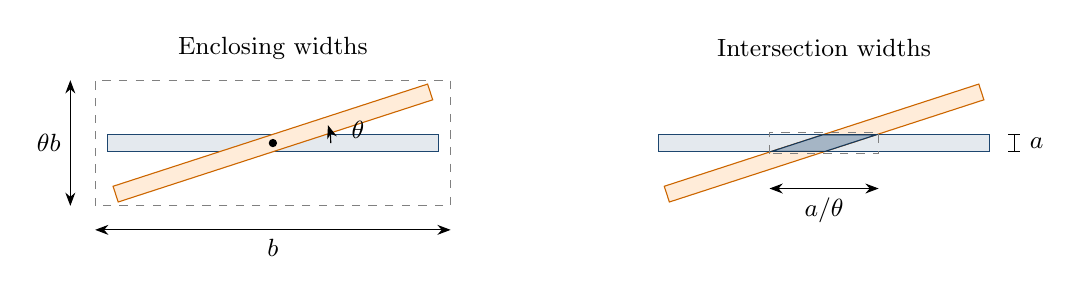
\begin{tikzpicture}[x=1.05cm,y=1.05cm,>=Stealth,font=\small]
\begin{scope}
\draw[dashed,gray] (-2.15,-.76) rectangle (2.15,.76);
\filldraw[fill=linkblue!12,draw=linkblue] (-2,-.10) rectangle (2,.10);
\begin{scope}[rotate=18]
\filldraw[fill=orange!15,draw=orange!80!black] (-2,-.10) rectangle (2,.10);
\end{scope}
\fill (0,0) circle (1.5pt);
\draw[->] (.7,0) arc[start angle=0,end angle=18,radius=.7];
\node at (1.03,.16) {$\theta$};
\draw[<->] (-2.15,-1.05)--(2.15,-1.05)
 node[midway,below] {$b$};
\draw[<->] (-2.45,-.76)--(-2.45,.76)
 node[midway,left] {$\theta b$};
\node at (0,1.15) {Enclosing widths};
\end{scope}
\begin{scope}[xshift=7cm]
\filldraw[fill=linkblue!12,draw=linkblue] (-2,-.10) rectangle (2,.10);
\begin{scope}[rotate=18]
\filldraw[fill=orange!15,draw=orange!80!black] (-2,-.10) rectangle (2,.10);
\end{scope}
\filldraw[fill=linkblue!40,draw=linkblue!80!black]
 (-.6314,-.1)--(.0158,-.1)--(.6314,.1)--(-.0158,.1)--cycle;
\draw[dashed,gray] (-.66,-.13) rectangle (.66,.13);
\draw[<->] (-.66,-.55)--(.66,-.55)
 node[midway,below] {$a/\theta$};
\draw (2.3,-.1)--(2.3,.1);
\draw (2.23,-.1)--(2.37,-.1);
\draw (2.23,.1)--(2.37,.1);
\node[right] at (2.37,0) {$a$};
\node at (0,1.15) {Intersection widths};
\end{scope}
\end{tikzpicture}
\caption{The transverse geometry in the adjacent-packet estimate,
schematically at comparable scales. A common assigned affine index ties
the packet centers together; the dot in the left panel represents its
trace. For $\theta\gg a/b$, the enclosing normal width is of order
$\theta b$, while the intersection of the two thin strips has length
of order $a/\theta$. Endpoint extrapolation and the adjacent scale
change contribute the $N^{O(\delta)}$ factors in the proof. All
dimensions in the diagram are understood up to constant factors.}
\label{fig:angle-packing}
\end{figure}


The factors omitted in the displayed quotient are changes of time
length, profile cost, and width type across one mesh step; their
logarithms are $O(\delta)$. If an extrapolated width passes the full
spatial size, cover it by the corresponding $N^{O(\delta)}$ bounded
planks. The same bound holds for event mass because the active indices
in a packet have uniform event counts on its block.

Since $y-x>0$, angles larger by a fixed positive exponent than $a/b$ can
be discarded with a power-small loss, after making $\delta$ sufficiently
small. Include the earlier packet partitions in the subsequent cleaning.
At cut $i$ the aspect exponent is $\kappa_i-\chi_i$, which is at least
$\kappa_i-F(\kappa_i)/v$. Summing the angular errors along the finite
chain, rather than adding their exponents, bounds the total angle by
$N^{-D_*(\kappa)+O(\delta)+o(1)}$. The final packet has one owner per
index on its physical block, so all retained initial plates of that
index on the block compare to the same final normal. Sending the mesh
to zero in the specified order proves the orientation assertion.

\paragraph{The inner equality.}
The reverse selection in Lemma~\ref{lem:derivative-capture} has
$\chi\ge F(s)/v$, while every admissible shape has $\chi\le s$.
Therefore $s-F(s)/v\ge0$. Its value at $s=\tau$ is $\tau$, proving the
bounds on $D_*$. Apply Lemma~\ref{lem:anisotropic} over the
$N^\kappa$-block with angular scale $\theta=N^{-D_*}$. Its fine assigned
plates are the flat-prefix plates of length $N^\tau$, and
$D_*\le\tau$ ensures $\theta\ge N^{-\tau}$. The effective resolution
is $N^{\kappa-D_*}$ and the raw lower multiplicity is
$mN^{D_*-o(1)}$. By the local upper bound its full-time plank parameter
is at most
\[
 mN^{-h\kappa-\Pi(\kappa)+yD_*}.
\]
Only an initial flat log interval of length $D_*$ is dropped. Multiplying
this parameter by the critical factor
$N^{h(\kappa-D_*)+\Pi(\kappa)}$ gives
$mN^{(y-h)D_*}=mN^{D_*}$, exactly the lower exponent. The normalized
profile thus gives \eqref{eq:inner-delay-deficit}. As for outer parents,
one can extract a representative equality from the aggregate chart
ensemble whenever this statement is used as a fact about equality
profiles.
\end{proof}

\subsection{A positive minimum delay and the canonical profile}

\begin{proposition}[Canonical equality profile]
\label{prop:canonical}
There is an exact equality whose profile is
\begin{equation}
 F(\kappa)=\beta(\kappa-\tau)_+,
 \qquad 0<\tau<1,\qquad
 \ell=1-\tau,\qquad \beta=v/\ell\le1.
 \label{eq:canonical-profile}
\end{equation}
Its deficit is $v$, and $\tau$ is the least initial delay among all
equalities with deficit $v$.
\end{proposition}

\begin{proof}
\emph{Attaining the maximal deficit.}
First, equalities with deficit $v$ exist. Start with any positive-deficit
equality and put $g(s)=s-F(s)/v$. If the running minimum of $g$ from
$\tau$ remained equal to $\tau$ throughout its nontrivial part,
Lemma~\ref{lem:angle-packing}, applied at a prefix with positive deficit,
would produce a nontrivial equality with zero initial delay. This
contradicts Lemma~\ref{lem:flat-delay}. There is therefore a new minimum
$D<\tau$, attained at a prefix $\kappa$ with
$g(\kappa)=D$. At this prefix the inner deficit is
\[
 \frac{F(\kappa)}{\kappa-D}=v.
\]
Let $\mathcal E_v$ denote the nonempty class of equality profiles with
deficit $v$, and set
\[
 \tau_* =\inf_{F\in\mathcal E_v}
             \sup\{r:F=0\text{ on }[0,r]\}.
\]

\paragraph{A positive lower bound for the delay.}
We claim that $\tau_*>0$. Suppose otherwise, and choose
$F_j\in\mathcal E_v$ with initial delays $\tau_j\to0$. Equality
compactness, as in Lemma~\ref{lem:hybrid-equality}, gives a subsequence
converging uniformly to an equality $F_\infty$ with deficit $v>0$.
The cost is lower semicontinuous; a strict downward jump would give a
violation of the critical inequality, so this limiting configuration is
still an equality. By Lemma~\ref{lem:flat-delay}, $F_\infty$ has a flat
interval of positive length.

The small-prefix multilinear argument underlying
Lemma~\ref{lem:prefix-extension} has slack depending only on the fixed
critical parameters. In particular, its allowed prefix length can be
chosen independently of the equality profile: the estimate used there is
\begin{equation}
 \frac{k^2m}{n}
 \ge N^{h+q+\Pi(1)-2\alpha-o(1)}
 \ge N^{h+(p-2)\alpha-o(1)}
 \ge N^{h-o(1)}.
 \label{eq:uniform-prefix-slack}
\end{equation}
Indeed $n\leexp\Delta_hN^d$,
$m\eqexp\Delta_hN^{h+\Pi(1)}$, and
$\Pi(1)\ge p\alpha-q$. Choose fixed $0<a_0<b_0$ inside both that
allowed prefix range and the flat interval of $F_\infty$.

For a sufficiently late $j$,
\[
 \tau_j<a_0,\qquad
 F_j(b_0)<\frac h4(b_0-a_0).
\]
Choose a minimizer $\kappa_j$ of $F_j(u)-(h/4)u$ on $[0,b_0]$.
At $b_0$ this function is strictly less than $-ha_0/4$, whereas for
$u\le a_0$ it is at least $-ha_0/4$. Hence $\kappa_j>a_0>\tau_j$,
so $\delta_j=F_j(\kappa_j)>0$. The minimizing property gives
\begin{equation}
 F_j(\kappa_j)-F_j(u)
 \le\frac h4(\kappa_j-u),\qquad 0\le u\le\kappa_j.
 \label{eq:late-prefix-record}
\end{equation}
Fix this particular $j$, its prefix $\kappa_j$, and its positive
$\delta_j$ before passing to the realizing resolution sequence.

Apply Lemma~\ref{lem:prefix-extension} to this fixed equality and
prefix, with $s=1-h/4$ and $\gamma=0$. Its uniform small-prefix
range includes $\kappa_j$, by the choice of $b_0$. The record inequality
\eqref{eq:late-prefix-record} is precisely its temporal hypothesis;
the other hypothesis is simply $F_j\ge0$. Its angular exponent is $h$,
so
\[
 t=1+3h/4,\qquad
 \mu=\min\{1,(s+t)/2,t\}=1.
\]
The lemma gives $\Pi(\kappa_j)\le F_j(\kappa_j)=\delta_j$.
But $\Pi(\kappa_j)\ge(p-1/2)\delta_j>\delta_j$, since
$\delta_j>0$ and $p>2$. This is a contradiction. The positive gap
is fixed after choosing $j$ and before taking its realizing resolution
to infinity; no uniform lower bound for the numbers $\delta_j$ is
needed. We have proved $\tau_*>0$.

\paragraph{Rigidity from the inner and outer delays.}
We now determine a profile attaining this infimum. For any
$F\in\mathcal E_v$ with initial delay $\tau$, $g(1)=0$. Given
$D'\in(0,\tau)$, let $s$ be the first passage below $D'$ after $\tau$:
\[
 s=\inf\{r>\tau:g(r)<D'\}.
\]
Continuity gives $\tau<s<1$, $g(s)=D'$, and
$\min_{\tau\le r\le s}g(r)=D'$. There are values below $D'$ arbitrarily
soon to the right of $s$. The inner equality from
Lemma~\ref{lem:angle-packing} has deficit $v$, so its delay is at least
$\tau_*$:
\begin{equation}
 \tau-D'\ge\tau_*(s-D').
 \label{eq:canonical-inner-passage}
\end{equation}

Any saturated outer cut at $s$ has $\chi\le s<1$ and deficit
$(v-F(s))/(1-\chi)$. By Lemma~\ref{lem:derivative-capture} this is at
most $v$, whence $\chi\le F(s)/v$. The reverse selection of that lemma
therefore attains $\chi=F(s)/v=s-D'$, and its outer deficit is exactly
$v$. Moreover $F$ increases arbitrarily soon to the right of $s$:
$g(r)<g(s)$ implies $F(r)-F(s)>v(r-s)$. Formula
\eqref{eq:outer-profile} consequently gives the exact outer delay
$D'/(1-s+D')$, not merely a lower bound for it. Its membership in
$\mathcal E_v$ yields
\begin{equation}
 D'\ge\tau_*(1-s+D').
 \label{eq:canonical-outer-passage}
\end{equation}

The two inequalities compare complementary rescalings of the same
profile, both with deficit $v$. For a sequence approaching the least
delay, they will force the same first-passage location.

Choose $F_j\in\mathcal E_v$ with $\tau_j\to\tau_*$. The Lipschitz
bound gives $v\le1-\tau_j$, so $\tau_*\le1-v<1$.
For each fixed $D'\in(0,\tau_*)$, the two passage inequalities give
\[
 1+D'-D'/\tau_*\le s_j
 \le D'+(\tau_j-D')/\tau_*.
\]
Thus
\[
 s_j\longrightarrow 1-\frac{1-\tau_*}{\tau_*}D',
 \qquad F_j(s_j)=v(s_j-D').
\]
Pass to a compact equality limit $F$. The rational values of $D'$ in
$(0,\tau_*)$ suffice; continuity then determines the profile at every
point above $\tau_*$. Below $\tau_*$ all these profiles vanish. We obtain
\[
 F(\kappa)=\frac{v}{1-\tau_*}(\kappa-\tau_*)_+.
\]
Its delay is exactly $\tau_*$ and its slope is at most one by the
Lipschitz bound. This proves \eqref{eq:canonical-profile}.
\end{proof}

Figure~\ref{fig:canonical-profile} shows the canonical profile and the
aspect exponent that controls its angular scale.

\begin{figure}[H]
\centering
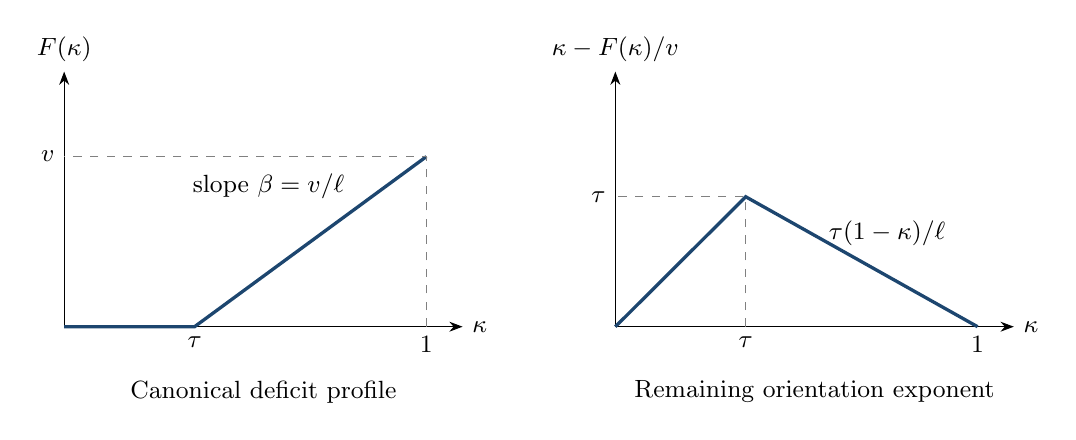
\begin{tikzpicture}[x=4.6cm,y=3.0cm,>=Stealth,font=\small]
\begin{scope}
\draw[->] (0,0)--(1.1,0) node[right] {$\kappa$};
\draw[->] (0,0)--(0,1.08) node[above] {$F(\kappa)$};
\draw[very thick,linkblue] (0,0)--(.36,0)--(1,.72);
\draw[dashed,gray] (1,0)--(1,.72)--(0,.72);
\node[left] at (0,.72) {$v$};
\node[below] at (.36,0) {$\tau$};
\node[below] at (1,0) {$1$};
\node[above left] at (.8,.5) {slope $\beta=v/\ell$};
\node[below=16pt] at (.55,0) {Canonical deficit profile};
\end{scope}
\begin{scope}[xshift=7.0cm]
\draw[->] (0,0)--(1.1,0) node[right] {$\kappa$};
\draw[->] (0,0)--(0,1.08) node[above] {$\kappa-F(\kappa)/v$};
\draw[very thick,linkblue] (0,0)--(.36,.55)--(1,0);
\draw[dashed,gray] (.36,0)--(.36,.55)--(0,.55);
\node[left] at (0,.55) {$\tau$};
\node[below] at (.36,0) {$\tau$};
\node[below] at (1,0) {$1$};
\node[above] at (.75,.3) {$\tau(1-\kappa)/\ell$};
\node[below=16pt] at (.55,0) {Remaining orientation exponent};
\end{scope}
\end{tikzpicture}
\caption{The canonical profile in Proposition~\ref{prop:canonical}.
After the flat interval, its slope is constant. For $\kappa\ge\tau$, the associated quantity
$\kappa-F(\kappa)/v$ decreases linearly from $\tau$ to zero;
at the stationary prefix $\kappa=1-\ell c$ it equals $\tau c$.
This identity gives the angular scale $\Theta_c=N^{-\tau c}$.
The vertical scales in the two panels are independent.}
\label{fig:canonical-profile}
\end{figure}


\subsection{Tracking a stationary shape}

Fix the canonical equality from Proposition~\ref{prop:canonical}. For
the remainder of the proof, $\ell$ always denotes $1-\tau$; the
logarithmic loss of an outer cut remains $\chi$.

\begin{lemma}[Canonical shape tracking]
\label{lem:stationary-shape}
For the canonical profile there are compatible finite chains, and slow
mesh limits of them, with cumulative shape parameters
\begin{equation}
 \kappa=\tau+\ell b',\qquad
 \chi=b',\qquad \mathfrak a=wb',\qquad
 w=h_z+\ell\mathcal D_q(q,\beta)\in(0,1],
 \quad 0\le b'<1.
 \label{eq:stationary-shape}
\end{equation}
The equalities in the parameters allow errors tending to zero with the
mesh. Packet mass, ownership, and orientation conclusions of
Lemmas~\ref{lem:nested-cuts} and~\ref{lem:angle-packing} remain valid.
\end{lemma}

\begin{proof}
An outer cut of a deficit-$v$ equality again has deficit at most $v$.
Applied to the canonical profile, this forces $\chi\le b'$. The reverse
derivative selection attains $\chi=b'$. Formula
\eqref{eq:outer-profile} then shows that the outer profile is the same
canonical profile: its flat delay is
\[
 \frac{\tau+\ell b'-b'}{1-b'}=\tau,
\]
and its nonflat slope is still $\beta$. The same statement applies
incrementally in every current outer model, in the original logarithmic
units.

For one mesh increment $\Delta b'$, the two coefficients in
\eqref{eq:derivative-capture}, written in those units, are
\[
 v(\Delta b'-\Delta\chi),\qquad
 h_z\Delta\chi+\ell\mathcal D_q(q,\beta)\Delta b'
                  -\Delta\mathfrak a.
\]
Every available saturation has $\Delta\chi\le\Delta b'$ by the outer
deficit bound. Take either sign of $\dot z$ and take $\dot p<0$ with
an arbitrarily large ratio $|\dot p|/|\dot z|$. First fix that ratio and
perform derivative capture. Along a subsequence as the ratio increases,
the nonnegative quantity $\Delta b'-\Delta\chi$ must tend to zero;
otherwise its negative $\dot p$ contribution cannot be offset by the
bounded second coefficient. The two signs of $\dot z$ therefore provide
choices with $\Delta\chi=\Delta b'$ and, respectively,
\[
 \Delta\mathfrak a\le w\Delta b',
 \qquad\text{or}\qquad
 \Delta\mathfrak a\ge w\Delta b'.
\]
Since $0\le\Delta\mathfrak a\le\Delta\chi$, this implies
$0\le w\le1$. Its defining expression and $h_z>0$ give $w>0$.

It is unnecessary to realize an exact intermediate shape on a single
step. If the running value of $\mathfrak a$ is above $wb'$, choose the
next increment from the lower side; if below, choose from the upper
side. The error can then overshoot zero by at most the mesh size, because
both $\Delta\mathfrak a$ and $w\Delta b'$ lie in
$[0,\Delta b']$. This tracks the desired total shape within one mesh
increment. The current outer profile stays canonical after each choice,
so both sides are available at every step. All perturbation limits are
resolved on a fixed finite chain before taking its mesh diagonal, and
Lemma~\ref{lem:nested-cuts} preserves the required earlier assignments.
\end{proof}

We now express the tracked packets in physical scales. Reverse the cut
parameter by $c=1-b'$ and put
\[
 \rho=1-w,\qquad B_*=h+\ell P_{p,q}(\beta),\qquad
 R_c=N^{-\ell c},\qquad\Theta_c=N^{-\tau c}.
\]
The corresponding logarithmic scale and cumulative shape are
\[
 \kappa=1-\ell c,\qquad \chi=1-c,\qquad
 \mathfrak a=w(1-c),\qquad \mathfrak u=\rho(1-c).
\]
For $0\le c\le1$, use nested dyadic time partitions whose blocks $I_c$
have physical length $R_c$, up to dyadic rounding. For
$0<c\le1$, write $B_c$ for its assigned packet. Its thin and thick
spatial widths in original cell units are
\begin{equation}
 a=N^{w(1-c)},\qquad
 b=N^{w+(\tau-w)c}.
 \label{eq:stationary-spatial-widths}
\end{equation}
At $c=1$ these are the initial flat-scale plates. As $c$ decreases,
the time blocks grow and the packets record the successive outer cuts.

For the probability statements, replace the finer events of each
occupied index--$I_1$ pair by one atom. More precisely, let
$\mathcal J_i$ be the occupied $I_1$ blocks on index $i$ and set
\[
 \Omega_* =\{(i,J):J\in\mathcal J_i\},\qquad
 Z_* =\sum_i\omega_i\#\mathcal J_i,\qquad
 \Prob\{(i,J)\}=\frac{\omega_i}{Z_*}.
\]
The atom $(i,J)$ is placed at the center $t_J$ of $J$ and carries the
spatial normal of the initial plate assigned to that index on $J$.
We restrict these normals to a fixed direction chart. After a fixed
orthonormal spatial change of coordinates, write their covectors as
$(1,\vartheta)$ with $\vartheta$ bounded. In the displayed law,
$\mathcal J_i$ and $Z_*$ refer to the retained pairs. Denote the atom's
time and normal coordinates by $e=(t,\vartheta)$, while retaining $i$
as a separate random variable. Nested dyadic quantization of $t$ and
$\vartheta$ at widths $R_c$ and $\Theta_c$ gives labels $e_c$.
The original uncollapsed equality supplies $m$, $\Delta_h$, and all
active-index plank bounds; this collapsed law supplies event probabilities.

In an event frame define the four matrix forms
\begin{equation}
 X=(1,\vartheta)\cdot M(t),\qquad Y=M(t)_2,
 \qquad U=(1,\vartheta)\cdot u,\qquad V=u_2.
 \label{eq:stationary-matrix-forms}
\end{equation}
Thus $X,U$ are normal position and velocity, and $Y,V$ are the fixed
complementary coordinates. This chart is generally oblique. Dividing
\eqref{eq:stationary-spatial-widths} by $N$ gives the spatial widths;
dividing again by the time length $R_c$ gives the velocity widths.
We write these four scales as
\begin{equation}
\begin{aligned}
 L_X(c)&=N^{-\rho-wc},&
 L_Y(c)&=L_X(c)\Theta_c^{-1},\\
 L_U(c)&=L_X(c)R_c^{-1},&
 L_V(c)&=L_X(c)(R_c\Theta_c)^{-1}.
\end{aligned}
\label{eq:estimate-widths}
\end{equation}
The proposition verifies that these widths remain valid in every used
event frame, and records the masses and branching of the same packets.

\begin{proposition}[Stationary data]
\label{prop:stationary-data}
There is a realizing sequence of canonical equalities and compatible
packet assignments for which the preceding collapsed law, event labels,
and matrix forms have the following properties. All local upper bounds
and original index weights are retained.
\begin{enumerate}[label=\textup{(\roman*)}]
\item
Along an index, occupied time blocks have regular branching exponent
$s_0=1-\beta\ge0$. More precisely, for fixed $c<b\le1$, an occupied
$I_c$ contains
\begin{equation}
 N^{\ell(1-\beta)(b-c)+o(1)}
 \label{eq:stationary-time-branching}
\end{equation}
occupied $I_b$ blocks. The event normals on that index in $I_c$ lie in a
range of size $\Theta_cN^{o(1)}$.

\item
For $0<c\le1$ there are assigned packets $B_c$ on the occupied $I_c$
blocks, with raw active index mass at least
\begin{equation}
 n_c=\Delta_h
 N^{(B_*+\tau)c+dw(1-c)}
 \label{eq:stationary-packet-mass}
\end{equation}
in exponent. On each fixed time block the assigned index sets are
disjoint, and each retained index has one packet owner there. The used
normals of a packet differ from its spatial normal by at most
$\Theta_cN^{o(1)}$.

\item
In every used event frame, the widths of $B_c$ in the four forms
\eqref{eq:stationary-matrix-forms} are bounded by
$L_X(c),L_Y(c),L_U(c),L_V(c)$ up to subpower expansion. Equivalently,
their negative log exponents are
\begin{equation}
 \rho+wc,\qquad \rho+(w-\tau)c,
 \qquad\rho+(w-\ell)c,\qquad\rho+(w-1)c,
 \label{eq:stationary-matrix-widths}
\end{equation}

\item
The data and packet lower bounds coexist on any prescribed finite list
of scales and tests, and hence on countable lists by slow diagonals. They
persist, in exponent, on typical nondeficient parts after extensive
regular refinements. All packet memberships are memberships of original
active indices on their physical intervals. In a chart registered at
$I_c$, the packet at a finer $I_b$ is determined by the index, chart, and
$I_b$; a matrix cell in that chart is determined by the index and chart.
\end{enumerate}
\end{proposition}

\begin{proof}
Choose the finite chains from Lemma~\ref{lem:stationary-shape} and
use the scales defined above.
On the canonical profile the running aspect exponent is decreasing
above $\tau$, and at $\kappa=1-\ell c$ its value is
\[
 \kappa-F(\kappa)/v=\tau c.
\]
The proof of Lemma~\ref{lem:angle-packing}, which applies unchanged to
the tracked finite chains, shows that every initial plate used by this
packet has its normal within $\Theta_cN^{o(1)}$ of the packet normal.
Since a packet is assigned only once to each index on its block, this
also gives the range assertion for all event normals on that index and
block. The canonical profile gives the number of occupied subblocks:
subtracting its deficits between the prefixes $1-\ell c$ and
$1-\ell b$ yields \eqref{eq:stationary-time-branching}.

We now verify the width bounds in the event frames.
The widths in \eqref{eq:estimate-widths} are first computed in the
packet's own normal frame. Changing to one of its used event normals
adds at most $\Theta_cN^{o(1)}$ times the transverse coordinate; the
ratios of transverse to normal widths are exactly $\Theta_c^{-1}$.
Changing the time center within $I_c$ adds at most $R_c$ times the
velocity coordinate. Both changes preserve the four widths up to
subpower factors.

For this profile,
\[
 \Pi(\kappa)=\ell(1-c)P_{p,q}(\beta),\qquad
 m\eqexp\Delta_hN^{B_*}.
\]
Substituting \eqref{eq:stationary-spatial-widths} in
\eqref{eq:stationary-local-threshold}, the exponent of the packet mass
relative to $\Delta_h$ is
\begin{align*}
 &B_*-\ell(1-c)P_{p,q}(\beta)-h(1-\ell c)
      +xw(1-c)+y\bigl(w+(\tau-w)c\bigr)\\
 &\hspace{12mm}=dw(1-c)
        +c\bigl(\ell P_{p,q}(\beta)+h\ell+y\tau\bigr)\\
 &\hspace{12mm}=dw(1-c)+(B_*+\tau)c,
\end{align*}
using $\ell+\tau=1$ and $y=1+h$. This proves
\eqref{eq:stationary-packet-mass}.

We next verify the passage to the collapsed law. Before collapse,
the number of finer events in every occupied index--$I_1$ pair has a
common exponent. Thus an extensive selection of atoms of weight
$\omega_i$ pulls back to an extensive selection of the uncollapsed
graph. Restricting the normal to one of finitely many direction charts
also retains an extensive piece, and normalized covectors and unit
normals are comparable on that chart. The orientation and time ranges
proved above imply that one index and $I_c$ use only subpower many
$e_c$ bins. Whenever the chart restriction or these labels split a
packet, retain nondeficient occupied pieces. The packet lower bounds
therefore survive for the law specified before the proposition.

For completeness, scale interpolation does not require new unrelated
assignments. At a finite mesh, use the packets already constructed.
A nearby intermediate interval is assigned the packet of its nearest
coarser mesh interval, restricted to the indices active in the smaller
interval. Extrapolation, width changes, and subdivision have
$N^{O(\text{mesh})}$ factors. Regular time counts and deficiency deletion
preserve the packet lower masses on typical occupied pieces. Along the
slow diagonal these factors are subpower. Alternatively, include any
specified intermediate scales in the next finite mesh. Thus a new
finite or countable list of scale tests can be accommodated by further
refinement, with the same limiting data.

Finally include, in the finite cleaning list, the assignment partitions
from every level in use. Lemma~\ref{lem:nested-cuts} then gives all the
simultaneous memberships, the original active-index interpretation, and
stability under extensive regular refinement in (iv). On a fixed
physical $I_b$, ownership was a decision for an index on that block;
after registration in a chart it is therefore constant on the tuple
specified in (iv). A cell of that chart's fixed matrix partition is
likewise a function only of the index and chart. The construction needs
outer steps only for $b'<1$, or $c>0$; it makes no cut at zero remaining
length. The endpoint $c=1$ is the initial assignment and has already been
included.
\end{proof}

We have proved $0<\tau<1$, $0<\ell<1$, $v>0$, and
$\beta=v/\ell>v$. The value $w=1$ is allowed, so that $\rho$ may
vanish. At this stage $\beta=1$ has not been excluded; the angular
estimate in the next section will show that $s_0=1-\beta$ is positive.

\section{Two estimates for the stationary configuration}
\label{sec:stationary-estimates}

We use the underlying equality and the collapsed event law of
Proposition~\ref{prop:stationary-data}. They have different purposes:
plank bounds always count inherited weights of original active indices,
whereas probabilities below are probabilities of indexed events. In
particular, restricting an event label does not restrict the reference
index mass in a plank test.

We prove two estimates. Lemma~\ref{lem:angular-frostman} bounds the
concentration of normal labels along an index and gives $\beta<1$.
Lemma~\ref{lem:conditional-X} bounds the additional normal-position
entropy inside a matrix cell after conditioning on a finer event label.
The first estimate follows by turning angular concentration into a
configuration with excessive temporal deficit. For the second, we
compare the mass of a queried packet with the original active-index
mass in its matrix cell, and then convert that comparison to entropy.

Throughout this section put
\[
 P=P_{p,q},\qquad x=d-1-h,\qquad y=1+h,
 \qquad x+y=d,\qquad y-h=1.
\]
The parameters $0<\tau,\ell<1$, $\tau+\ell=1$, $v>0$,
$\beta=v/\ell\le1$, and $0<w\le1$ are fixed. Thus
$\beta>v$, including before we exclude $\beta=1$.

Recall the four matrix widths $L_X(c),L_Y(c),L_U(c),L_V(c)$ from
\eqref{eq:estimate-widths}. For a coarse event label
$e_c=(t_c,\vartheta_c)$, evaluate the four forms at its chosen center.
For a real offset $a$, let $Q(c,a)$ be their joint matrix-cell label
at those widths multiplied by $N^{-a}$. The grids are dyadic, with the usual
bounded enlargements at rounded scales. Conditional on $e_c$, this is
a partition of the matrix indices; repetitions at the same matrix
retain their individual weights. All limits first fix the scale
parameters and any strict exponent margin, and then let $N\to\infty$.
Finite lists of such tests precede the countable diagonals.

\subsection{Mass accounting for the selections}

Both proofs select events and then fill the occupied time blocks they
meet. We must retain the packet mass and control the change in the time
profile under the same selection. The following form of finite cleaning
does this even when the selection has a fixed power loss. Its essential
distinction is between original packet masses, against which that loss
is measured, and the restricted graph on which new probability labels
are computed.

\begin{lemma}[Cleaning registered events]
\label{lem:estimate-cleaning}
Let a finite weighted event graph have total weight $W$, and let a
restriction retain weight at least $N^{-E+o(1)}W$. Fix finitely many
partitions of the graph. The cells may include packet assignments,
index--time blocks, and joint labels. After a further restriction of
subpower cost, every surviving
cell of each partition retains at least $N^{-E-o(1)}$ of its original
weight. The same assertion holds after splitting each original cell
among subpower many registered charts, with that number absorbed in
the error.

Suppose, in addition, that the original time trees have a common
profile $F$ on a log interval $[0,\Lambda]$ in $\log N$ units, and each
original index and starting interval is routed through only subpower
many charts. If the restricted trees are made uniform, with profile
$G$, then
\begin{equation}
 G(t)-G(s)\ge F(t)-F(s),\qquad
 0\le G(\Lambda)-F(\Lambda)\le E,
 \quad 0\le s<t\le\Lambda.
\label{eq:estimate-branch-loss}
\end{equation}
In particular an extensive restriction preserves the profile, and
\begin{equation}
 0\le \int_0^\Lambda P(G')-\int_0^\Lambda P(F')\le pE.
\label{eq:estimate-cost-loss}
\end{equation}
These assertions concern inherited index weights.
\end{lemma}

\begin{proof}
We distinguish two reference graphs in the cleaning. For the new
homogenization tests use the finite label construction of
Lemma~\ref{lem:regularization}: these are its within-index integer
counts and conditional-probability tests with polynomially many
children. Perform its negligible conditional-probability tail
deletions before computing the labels. Arbitrary-cardinality original
packet partitions are retained only as cleaning tests; no absolute
weight label is imposed on their cells. Let $W$ be the original event
weight and let $R$ be the restricted, routed graph after those tail
deletions and before the finite labels are selected. Write $M_0=|R|$;
thus $M_0\ge N^{-E-o(1)}W$. Compute the prescribed rounded labels
on $R$, including their joint and domain tests for conditional counts,
and retain one common finite list of labels. All graph masses denoted
by $|\cdot|$ here and in the registration rule below are weighted
event masses. Denote this label
class by $A$, and write $M=|A|$. The number of label lists is subpower,
so $M\ge N^{-o(1)}M_0\ge N^{-E-o(1)}W$. Counts within index fibers
are event counts, with the inherited index weight cancelling in their
ratios. No bound on the number of distinct weighted indices is required.

There are two collections of reference masses. Original packet,
index--time, and chart tests use their masses in the original graph;
the sum of these references is at most $L_{\rm old}W$.
New regularization tests use their masses in $R$, the graph on which
their labels were computed; their reference sum is at most
$L_{\rm new}M_0$. Here $L_{\rm old},L_{\rm new}=N^{o(1)}$
include the finite number of partitions and any subpower chart copies.
In particular, one does not substitute the possibly much smaller
post-label cell mass for an $R$-reference without recomputing its label.

Choose $\epsilon_N\downarrow0$ slowly enough to dominate the label
loss $\log_N(M_0/M)$, the error in $M\ge N^{-E-o(1)}W$, and the
$\log_N L_{\rm old}$ and $\log_N L_{\rm new}$, with margins tending to
infinity after multiplication by $\log N$. Starting from $A$, delete
all events in a deficient original-reference cell when its current
mass is less than $N^{-E-\epsilon_N}$ times that reference. For a
new regularization cell or domain, use instead $N^{-\epsilon_N}$
times its $R$-reference. Continue either type of deletion until no
deficient cell remains. A cell is charged only once, because it is
empty after deletion. Even with cascades, the two total charges are
at most
\[
 L_{\rm old}N^{-E-\epsilon_N}W=o(M),\qquad
 L_{\rm new}N^{-\epsilon_N}M_0=o(M).
\]
The final graph therefore has mass $(1-o(1))M$. Every surviving old
cell retains at least $N^{-E-o(1)}$ of its original mass. Every
surviving new cell retains $N^{-o(1)}$ of its $R$-mass and is a
subset of that cell, so the rounded exponents selected from $R$
remain valid, including conditional exponents obtained by ratios of
joint and domain masses. This proves the mass assertion: the new labels
incur only a subpower loss in addition to the original loss $E$. The
finite-test diagonal allows further prescribed tests.

For the profile assertion fix a finite mesh of time scales and
uniformize the branching counts on its gaps. A subtree cannot have
more children on any gap than the original tree. Since the branching
exponent on $[s,t]$ is $(t-s)-(F(t)-F(s))$, this proves the first
inequality in \eqref{eq:estimate-branch-loss}. The total available
index weight after routing is at most $N^{o(1)}$ times its original
value. Comparing this with the retained weighted event count shows
that the number of events per surviving uniform index is at least
$N^{-E-o(1)}$ times the original number. This proves the endpoint
inequality. Refine the fixed mesh only after these comparisons hold.
The Lipschitz profile limits give \eqref{eq:estimate-branch-loss} on
every interval, hence $G'\ge F'$ almost everywhere and
$\int(G'-F')\le E$. The function $P$ is increasing and has Lipschitz
constant at most $p$, which proves \eqref{eq:estimate-cost-loss}.
\end{proof}

Here is the registration rule used below. Before any restriction, an
occupied time block $J$ on an assigned index has a common number
$m_J=N^{\kappa+o(1)}$ of finer events, uniformly in the blocks under
consideration. Given a selected set of finer events, first register
every occupied token $(i,J)$ that it hits, giving that token weight
$\omega_i$, and complete its block. Any preassigned chart or other
label on which the predicate depends remains part of its token;
completion never changes that label. Subpower many such tags enlarge
the original reference totals by only a subpower factor. If $T_0$ is the original token
weight and $T$ the weight of the registered tokens, then
\[
 |\text{selected finer events}|
 \le N^{\kappa+o(1)}T,\qquad
 |\text{original finer events}|=N^{\kappa+o(1)}T_0.
\]
Consequently a restriction of finer-event weight $N^{-E-o(1)}$
registers at least $N^{-E-o(1)}T_0$ token weight. Completing these
tokens precedes chart splitting and incurs no further loss. Route
whole tokens through their geometric charts; each original index and
starting block has only subpower many such charts. If it is necessary
to prune chart portions, compare them with their masses in this
restricted, completed token graph, rather than with the original
unrestricted block's finer-event mass. Portions below
$N^{-\epsilon_N}$ of their restricted unsplit reference have total
weight $o(T)$ after choosing $\epsilon_N$ slowly. A predicate constant
on $(i,J)$ is unchanged by completion or later filling. The original
packet references are still the unrestricted assigned token masses,
and keep the $N^{-E-o(1)}$ threshold in the preceding two-budget
cleaning. Thus this registration retains both the original packet
lower bounds and the single event-retention loss $E$.

\subsection{Angular nonconcentration}

\begin{lemma}[Angular Frostman bound]
\label{lem:angular-frostman}
There is $\gamma>0$, depending only on the fixed stationary parameters,
with the following property. For every fixed $0<c<b\le1$, outside a
set of index--$I_c$ fibers of event probability tending to zero, every
angular interval $J$ of length $\Theta_b$ satisfies
\begin{equation}
 \frac{\#\{e\text{ on }i:t(e)\in I_c,
                         \ \vartheta(e)\in J\}}
      {\#\{e\text{ on }i:t(e)\in I_c\}}
 \le N^{-\gamma\tau(b-c)+o(1)}.
\label{eq:angular-frostman}
\end{equation}
It is enough to test a fixed grid with bounded enlargements. The bound
also holds conditional on typical nondeficient $e_c$ bins in the fiber,
and after extensive regular refinements. In particular
\begin{equation}
 0<\beta<1,\qquad s_0=1-\beta>0.
\label{eq:positive-time-dimension}
\end{equation}
\end{lemma}

\begin{proof}
Angular concentration would produce a configuration whose normalized
temporal deficit is at least $\beta$. Since $\beta>v=-h_p$, decreasing
$p$ makes the critical upper bound for that configuration strictly
smaller than its packet lower bound. We quantify how close the two
bounds remain after selecting a narrow angular bin: a selection loss
$E$ decreases the packet mass by at most $E$ in exponent and increases
its temporal cost by at most $pE$.

Write $g=b-c>0$ and
\[
 S=n_bN^{-\tau b},\qquad K'=N^{b-\ell c},
 \qquad\theta=\Theta_b=N^{-\tau b}.
\]
First pass to the isotropic outer parents associated to $B_b$, as in
Lemma~\ref{lem:nested-cuts}. Their effective resolution count is
$N^b$. The assigned $B_b$ plates have time and long spatial length
$N^{\tau b}$ in these cell units, unit thin width, and mass at least
$SN^{\tau b-o(1)}$. On the longer interval $I_c$, which has $K'$ bins
in this model, the local bound of Proposition~\ref{prop:local-bound}
pulls back to
\begin{equation}
 n(\text{plank of widths }a_1,b_1)
 \le N^{o(1)}
 S N^{-\ell gP(\beta)}(K')^{-h}a_1^xb_1^y.
\label{eq:angular-parent-bound}
\end{equation}
For example, the isotropic physical cell width is
$N^{w(1-b)}$ in original cell units. Substitution in the original
local bound gives the coefficient
\[
 mN^{-\ell(1-c)P(\beta)}N^{-h(1-\ell c)}
       N^{dw(1-b)}
 = S N^{-\ell gP(\beta)}(K')^{-h}
\]
in exponent, using $m\eqexp\Delta_hN^{B_*}$ and
\eqref{eq:stationary-packet-mass}. Thus
\eqref{eq:angular-parent-bound} counts original active indices; it is
not a bound only for indices occupying a selected angular bin.

Suppose that fibers violating \eqref{eq:angular-frostman} account for
an extensive event piece. On each such index and $I_c$ choose one
violating bin and keep its events. This costs at most
\[
 E=\gamma\tau g
\]
in log probability, apart from a vanishing error. First register and complete every occupied $I_b$ token hit by this
selection, before any chart-portion cutoff. The preceding registration
rule gives token weight at least $N^{-E-o(1)}$ of the original token
graph. The normal of its assigned $B_b$ packet is within
$\Theta_bN^{o(1)}$ of the selected bin, since the packet contains the
event that registered the token and its normal label is constant on
the token. Completing the block does not change its packet owner.
Route these whole tokens through the outer parents and bin choices.
Each packet has only subpower many relevant choices, and each index
on $I_c$ has only subpower many charts. Any deficient chart portions
are pruned relative to this restricted token graph. Now apply the
two-budget cleaning of Lemma~\ref{lem:estimate-cleaning}: original
packet and time-tree references use the loss $E$, while the new
homogenization references, computed after registration and routing,
use only a subpower loss. The final token graph still has weight
$N^{-E-o(1)}$ of the original one, and each surviving packet has raw
assigned mass at least
\begin{equation}
 SN^{\tau b-E-o(1)}.
\label{eq:angular-selected-packet}
\end{equation}
The uniform token trees are subtrees of the original occupied
$I_b$ trees below $I_c$, with subpower many routed copies. Thus their
endpoint deficit loss is at most $E$ and their cost increase is at
most $pE$. Packet loss $E$ and cost increase $pE$ are the two
consequences of this same retained graph; the selection is not
performed a second time.

Apply the geometric construction in the proof of
Lemma~\ref{lem:anisotropic} on $I_c$, with angular width $\theta$.
Here we use only its bounded-chart routing, rectangle pullback, and
cell-count calculation. That calculation is linear in the packet
mass, which here is the reduced value $SN^{\tau b-E-o(1)}$ from
\eqref{eq:angular-selected-packet}. We do not use that lemma's
profile-preservation conclusion for an extensive graph: the endpoint
loss $E$ and cost increase $pE$ were proved by
Lemma~\ref{lem:estimate-cleaning} and are used explicitly in
\eqref{eq:angular-cost} below. The resulting normalization has resolution
\begin{equation}
 N_{\mathrm{new}}=K'\theta=N^{\ell g}.
\label{eq:angular-new-resolution}
\end{equation}
The selected plates become bounded-cell packets: their old time and
long spatial length multiplied by $\theta$ is one, and their
orientation error is $N^{o(1)}\theta$. Filling their occupied $I_b$
blocks before this normalization therefore gives aggregate raw
multiplicity at least the quantity in
\eqref{eq:angular-selected-packet}. The full-plank parameter of the
new models is at most
\begin{equation}
 \Delta_{\mathrm{new},h}
 \le N^{o(1)}S N^{-\ell gP(\beta)}(K')^{-h}\theta^{-y}.
\label{eq:angular-new-clustering}
\end{equation}
Here the factor $\theta^{-y}$ follows by pulling back a rectangle:
its area expands by $\theta^{-1}$ and its largest width by at most
$\theta^{-1}$, and $a^xb^y=(ab)^xb^{y-x}$ with $0\le x\le y$.

We next quantify the time cost. Prior to selection the occupied
$I_b$ blocks below $I_c$ have constant deficit slope $\beta$ over a
log interval of length $\ell g$. Filling and then normalizing removes
only the flat range below them. The restricted uniform time tree
cannot gain branching on any fixed gap. Its normalized deficit
$\alpha_{\mathrm{new}}$ is therefore at least $\beta$. By
\eqref{eq:estimate-cost-loss}, its cost, expressed in $\log N$ units,
is at most
\begin{equation}
 \ell gP(\beta)+pE+o(1).
\label{eq:angular-cost}
\end{equation}
The comparison uses the whole routed ensemble: the number of chart
copies per original index and $I_c$ is subpower, so the total
branching loss is at most $E$, as in the proof of
Lemma~\ref{lem:estimate-cleaning}.

Without the controlled losses, the sharp upper bound from
Definition~\ref{def:critical} and
\eqref{eq:angular-new-clustering} matches $SN^{\tau b}$ exactly.
Indeed its exponent relative to $S$ is
\begin{align*}
 -\ell gP(\beta)-h(b-\ell c)+y\tau b
       +h\ell g+\ell gP(\beta)
 &=\tau b.
\end{align*}
Thus \eqref{eq:angular-selected-packet} and
\eqref{eq:angular-cost} place the new models within
$(p+1)E+o(1)$ of their sharp upper bound in $\log N$ units.

Choose a small fixed $t_*>0$ with $p-t_*>2$ and
\begin{equation}
 0\le h(p-t_*,z)-h(p,z)
 \le \frac{v+\beta}{2}\,t_*.
\label{eq:angular-p-perturbation}
\end{equation}
This is possible by differentiability and $\beta>v$.
Increasing $h$ at fixed $d$ cannot increase the plank parameter,
because its value on a plank is multiplied by
$(a_1/b_1)^{h'-h}\le1$. Also
$P_{p-t_*,q}(e)=P_{p,q}(e)-t_*e$. Applying the critical bound at
$(p-t_*,z)$ to these same models therefore saves at least
\[
 N_{\mathrm{new}}^{(\beta-v)t_*/2}
\]
relative to the old sharp upper estimate. Choose once and for all
\begin{equation}
 0<\gamma<\min\left\{
 \frac12,\frac{\ell(\beta-v)t_*}{8(p+1)\tau}
 \right\}.
\label{eq:angular-gamma-choice}
\end{equation}
The saving then strictly exceeds the error $(p+1)E$. This contradicts
the aggregate lower multiplicity. Uniformity over bounded parent
charts follows from the uniform all-configuration critical bound;
otherwise a parent subsequence would violate that bound.

It follows that the violating fibers are not an extensive piece.
In particular their probability tends to zero. This proves
\eqref{eq:angular-frostman} for each fixed gap. The choice
\eqref{eq:angular-gamma-choice} is independent of $b-c$: both the
selection loss and the strict saving were proportional to that gap
before normalization. Fix finitely many gaps first and absorb their
errors; the diagonal convention then gives all required scale tests.

Within an index and $I_c$ the normals occupy only subpower many
$e_c$ bins. Delete bins retaining less than a subpower fraction of the
fiber, by the same deficiency argument. Dividing by their remaining
mass changes \eqref{eq:angular-frostman} by only a subpower factor.
An extensive subsequent regular refinement has the same property by
Lemma~\ref{lem:estimate-cleaning}.

Finally suppose $\beta=1$. For any fixed $0<c<1$, an occupied
index--$I_c$ fiber has only $N^{o(1)}$ occupied $I_1$ blocks by
\eqref{eq:stationary-time-branching}, and there is one collapsed
event per such block. One angular bin of width $\Theta_1$ therefore
has at least $N^{-o(1)}$ of its event mass. This contradicts
\eqref{eq:angular-frostman} at $b=1$, since $\gamma\tau(1-c)>0$.
Hence $\beta<1$; positivity follows from $v>0$.
\end{proof}

\subsection{Conditional concentration in the normal position}

We next compare a queried packet with the original active-index mass
in its matrix cell. This reference mass includes indices whose shadings
do not carry the query's finer event label. A lower bound for such a
reference mass can nevertheless bound the query's entropy: entropy is
at most cross-entropy against any positive reference probability. The
proof first establishes the geometric mass bound and then applies this
inequality to the normal-position observation.

For a finite random variable write
$\mathrm H_N(Z\mid L)=\mathrm H(Z\mid L)/\log N$, using natural
logarithms. If $L=e_{c+\sigma}$, let $X_L$ be the normal-position
form evaluated at the center of that finer label. Let
\[
 [X_L]_{c,a+\Delta}
\]
denote its grid bin at width $L_X(c)N^{-a-\Delta}$. Its grid may be
translated by a quantity determined by $Q(c,a)$ and $L$; changing
between such grids changes the conditional entropy by $O(1)$.

\begin{lemma}[Conditional $X$ estimate]
\label{lem:conditional-X}
Fix $0<c<1$, $0<a<w(1-c)$, and $\sigma>0$ with
$c+\sigma\le1$. For all sufficiently small fixed $\Delta>0$,
\begin{equation}
 \limsup_{N\to\infty}
 \mathrm H_N\bigl([X_{e_{c+\sigma}}]_{c,a+\Delta}
                  \mid Q(c,a),e_{c+\sigma}\bigr)
 \le x\Delta.
\label{eq:conditional-X-bound}
\end{equation}
For example it suffices to take
\begin{equation}
 0<\Delta<\frac14\min\left\{
 a,\ w(1-c)-a,\ \frac{\tau a}{w},\
 \min(\tau,\ell)\sigma
 \right\}.
\label{eq:conditional-X-admissible}
\end{equation}
The assertion holds for the event law on any extensive regular
refinement, with the original active-index masses still available as
reference masses. The limit in $N$ precedes limits in $\Delta$ or
$\sigma$.
\end{lemma}

\begin{proof}
The geometric argument uses coarse matrix cells within registered
charts. We will replace each cell by its center, weighted by the full
original active-index mass in that cell, and regard the selected
original indices as its children. After selecting a common ratio of child mass
to representative mass, their normalized event laws are comparable.
The critical inequality bounds the representatives' multiplicity,
whereas packet saturation gives a lower bound for the children's mass
in a typical spatial cell. These bounds force a typical packet to
contain a sufficiently large fraction of its queried cell's reference
mass. We first construct the charts in which this comparison is made.

Put
\begin{equation}
 g=b-c=\frac{a+\Delta}{w},\qquad
 D_0=N^g,\qquad D=N^\Delta,\qquad
 Z'=N^{\tau g},\qquad S'=\frac{n_b}{Z'}.
\label{eq:X-test-parameters}
\end{equation}
The conditions \eqref{eq:conditional-X-admissible} imply
$c<b<1$ and $\Delta<\tau g$, so a positive flat range remains in
the time filling used below.

\paragraph{Chart geometry.}
Fix $e_c$ and its interval $I_c$. In its frozen frame normalize time
by $R_c$, spatial normal and transverse position by
$R_c\Theta_c,R_c$, and velocity by the corresponding spatial units
divided by $R_c$. In these coordinates a $Q(c,a)$ cell has isotropic
matrix diameter, up to dimension constants,
\[
 N^{-\rho(1-c)-a}.
\]
Take isotropic matrix parents of diameter $N^{-\rho(1-b)}$, subtract
their centers, and divide the spatial and velocity coordinates by
that diameter. The resulting charts are bounded and have resolution
$D_0^{-1}$. In each such parent, the diameter of a cell of
$Q(c,a)$ is
\begin{equation}
 N^{-\rho(b-c)-a}=N^{-g+\Delta}=D/D_0.
\label{eq:X-cell-diameter}
\end{equation}
We used $wg=a+\Delta$ in the equality. One may choose compatible
nested grids; if a prescribed cell meets a parent boundary, splitting
it among boundedly many parents adds only $O(1)$ entropy at the end.
Hereafter $C$ denotes the resulting cell within its registered chart,
including this subdivision when needed.

A $B_b$ packet fits in subpower many of these charts. Its used
normals lie in $\Theta_bN^{o(1)}$, hence in subpower many $e_c$
bins, and its four width bounds extrapolated from $I_b$ to $I_c$
have matrix diameter at most $N^{-\rho(1-b)+o(1)}$ in the
$I_c$ normalization. Use the packet's own normal and its own time center for the following
four widths after parent normalization. Their negative log exponents
are
\begin{equation}
 (g,\ell g,\tau g,0).
\label{eq:X-normalized-packet-widths}
\end{equation}
In the normalized $I_c$ chart the change of normal is
$(\vartheta_P-\vartheta_c)/\Theta_c=O(1)$, and the change of time
center is $(t_P-t_c)/R_c=O(1)$. These are bounded shears. They need
not preserve the four coordinate widths in the frozen $e_c$ frame;
they preserve the following geometric bounds, up to fixed factors.
At resolution $D_0$ the packet is a plate of thin spatial width one
cell, long spatial width $Z'$, and time length $Z'$ bins, with raw
assigned mass at least $S'Z'N^{-o(1)}$.
Each index and $I_c$ is in only subpower many registered charts.
After chart splitting, Lemma~\ref{lem:estimate-cleaning} preserves
these packet masses on typical occupied pieces.

\paragraph{The reference-mass claim.}
For each cell $C$ in a registered chart define
\begin{equation}
 n_C=\sum_{\substack{i\text{ active on the original }I_c\\M_i\in C}}
                   \omega_i.
\label{eq:X-reference-mass}
\end{equation}
For a packet $P=B_b$ on an $I_b$ block, write $n(C\cap P)$ for
the inherited mass of its assigned active indices that lie in $C$.
We will prove that, outside a set of query events of probability
tending to zero,
\begin{equation}
 n(C\cap P)\ge n_C D^{-x-o(1)}.
\label{eq:X-reference-packet}
\end{equation}
The claim also holds if the query events were first restricted to an
extensive regular piece, with the same full original active mass in
\eqref{eq:X-reference-mass}. This reference mass belongs to the chart cell
$C$ just defined.

The critical comparison uses the following inherited bound. Let
$\Delta_0$ denote the full-time plank parameter in
one of these bounded normalized charts, with exponents $x,y$. Its
physical normal cell width in original cell units is $N^{w(1-b)}$;
the transverse cell width is
$\Theta_c^{-1}N^{w(1-b)}$. Pulling back an arbitrarily oriented
rectangle multiplies its area by
$N^{2w(1-b)}\Theta_c^{-1}$ and its largest width by at most
$N^{w(1-b)}\Theta_c^{-1}$. Since $0\le x\le y$, the original
local estimate gives
\begin{align}
 \Delta_0
 &\le N^{o(1)}mN^{-\ell(1-c)P(\beta)}
       N^{-h(1-\ell c)}N^{dw(1-b)}\Theta_c^{-y}
       \notag\\
 &\eqexp S'D_0^{-B_*}.
\label{eq:X-chart-clustering}
\end{align}
For the last equality, its exponent relative to $\Delta_h$ is
$cB_*+\tau c+dw(1-b)$; the same exponent results from
$S'D_0^{-B_*}$ using \eqref{eq:stationary-packet-mass}.
All these bounds count original indices active on $I_c$, whether or
not those indices carry the particular normal label used to name
the chart. An upper bound for a subcollection is therefore inherited
without changing the reference weights.

\paragraph{Registering the failed queries.}
Suppose the reference-mass claim fails. After a subsequence, for some
fixed $\epsilon>0$
the events satisfying
\begin{equation}
 n(C\cap P)<n_CD^{-x}N^{-\epsilon}
\label{eq:X-bad-predicate}
\end{equation}
form an extensive piece. Register tuples $(i,\mathfrak c,J)$,
where $\mathfrak c$ specifies the chart, including $e_c,I_c$ and
the parent, and $J=I_b$ is occupied. Give each tuple weight
$\omega_i$. The cell $C$ is fixed by $(i,\mathfrak c)$, and its
packet owner is fixed by $(i,\mathfrak c,J)$, by
Proposition~\ref{prop:stationary-data}(iv). Consequently
\eqref{eq:X-bad-predicate} is constant on the tuple. This constancy
is the reason that replacing its finer events by a token and later
filling $J$ does not change the failed test.

Before selection each occupied $J$ has a common number of original
events in exponent. Register every tuple $(i,\mathfrak c,J)$ hit by
a bad query and complete its $J$ block in that fixed chart, before
chart-portion pruning. The chart component is retained throughout:
the failed predicate depends on it. Because the predicate is constant
on this tuple, completion preserves it. The
bad tuples consequently have extensive inherited weight in the
original token graph. Any chart cutoff is taken relative to the
restricted completed token graph; there are only subpower many
chart portions per index and $I_c$. Clean the packet partitions,
using the original token masses for packet references and the graph
where labels were computed for new regularization references.
The registered assigned mass of each surviving packet in a chart
is then at least $S'Z'N^{-o(1)}$. The assigned index sets are
disjoint for a fixed chart and $J$.

\paragraph{Frequency selection.}
We next make the selected child mass comparable to the reference mass
by a common factor. This will allow a multiplicity estimate sampled
under the representative law to be used for the child events.
On the retained tuple graph define
\[
 \mathsf w(C,J)=
   \sum_{\substack{(i,\mathfrak c,J)\text{ retained}\\M_i\in C}}
         \omega_i.
\]
This is at most $n_C$. Select one common exponent of
$\mathsf w(C,J)/n_C$ across the ensemble. Here is the finite
justification even when the original weights are arbitrarily
unequal. There are polynomially many charts, cells, and time blocks,
and each $n_C\le n$. If their total number is at most $N^A$,
ratios below $N^{-A-3}$ contribute at most $N^{-3}n$ to the tuple
weight and may be discarded. The extensive original token graph has
weight at least $nN^{-o(1)}$: every original index had a common total
event count, and the restriction cannot create more events per
index. Partition the remaining logarithmic ratios in $[0,A+3]$ on
a mesh tending slowly to zero. There are subpower many levels, so
one retains an extensive level. After further cleaning the
$(C,J)$ cells, using their masses at this level as references,
there is an exponent $r\ge0$ such that
\begin{equation}
 \frac{\mathsf w(C,J)}{n_C}=N^{-r+o(1)}
\label{eq:X-frequency}
\end{equation}
uniformly on all surviving pairs. It is the selected
$\mathsf w(C,J)$, not $n_C$, that is used as the reference for this
deficiency deletion. Therefore the sum of reference masses in this
cleaning partition is the tuple weight, not a possibly much larger
sum of $n_C$'s. Include the packet cells and all prescribed time-tree
tests in the same deletion process. The packet lower masses, the
ratio \eqref{eq:X-frequency}, and the inherited uniform child
branching then hold simultaneously.

\paragraph{Representatives and their event law.}
Fill every registered tuple over its whole interval $J$ and rebin
time at the coarser resolution
\[
 (D_0/D)^{-1}.
\]
Each $J$ contains $Z'/D$ such bins, up to the harmless dyadic
rounding, and this number has positive exponent. The operation
drops only part of the full-branching range grafted below $J$.
For each occupied $C$ put one representative matrix at its center,
of weight $n_C$. Occupy that representative at every coarse time
bin belonging to a registered pair $(C,J)$. Charts are counted
separately. A child tuple at a coarse bin is assigned to the spatial
cell hit by its representative at that bin center; this is the
hashing used in the argument.

On each representative event the total weight of its children is
$\mathsf w(C,J)$. By \eqref{eq:X-frequency}, the ratio of that
weight to the representative weight is $N^{-r+o(1)}$, uniformly.
The same common factor compares the total masses. Thus the two
normalized event laws are mutually dominated up to subpower
factors. In particular, an extensive set of representative events
pulls back to an extensive set of interpolated child events. This
statement does not identify the individual index weights $n_C$
with the child weights.

\paragraph{The representative multiplicity bound.}
We apply the critical inequality to this representative configuration.
Its plank parameter is inherited from the reference indices; its
temporal cost will be bounded using the selected children.
The full-plank parameter for this representative model is at most
\begin{equation}
 \Delta_{\mathrm{rep},h}
 \le N^{o(1)} S'D_0^{-B_*}D^d.
\label{eq:X-representative-clustering}
\end{equation}
Indeed, by \eqref{eq:X-cell-diameter}, every original line counted
in $n_C$ stays within a bounded coarse cell of the representative
throughout the whole normalized time interval. A coarse plank
containing the representative therefore contains all these lines
after bounded enlargement. In the old $D_0$ cell units its widths
are at most constant multiples of $Da_1,Db_1$. The cells $C$
partition the original active indices within a chart, so summing
their weights does not duplicate any index in that chart. Apply
\eqref{eq:X-chart-clustering} and use $x+y=d$ to obtain
\eqref{eq:X-representative-clustering}.

We claim that the sum of the occupied representative weights in a
typical hashed space--time cell is at most
\begin{equation}
 S'D^{d-h}N^{o(1)}.
\label{eq:X-representative-multiplicity}
\end{equation}
If cells with a strict excess carried extensive representative
incidence weight, restrict to those cells. Their aggregate support
is at most their weighted incidence count divided by the proposed
excess threshold. Make the representative time profiles uniform
over the ensemble, retaining an extensive piece.

It remains to bound the cost of this profile. Up to the
creation of representatives, all selections (the bad predicate,
chart routing, frequency-level selection, and their regularizations)
are extensive restrictions of inherited-weight child tokens. The
reference mass $n_C$ used to define the frequency ratio never becomes
a child index weight. Filling each registered $J$ adds the same
$Z'/D$ coarse events per token. It follows from
Lemma~\ref{lem:estimate-cleaning}, on every tested gap, that the
interpolated children have profile
\begin{equation}
 F_{\mathrm{ch}}(\kappa)
 =\beta\bigl(\kappa-(\tau g-\Delta)\bigr)_+,
 \qquad 0\le\kappa\le g-\Delta.
\label{eq:X-child-profile}
\end{equation}
The bottom interval is filled and has zero cost, and the remaining
interval has length $\ell g$.

Keep the extensively restricted and regularized representative graph
fixed from now on. Pull its event restriction back to its children.
Equation~\eqref{eq:X-frequency} compares normalized representative
and child event weights by subpower factors on every event, so this
pullback is an extensive restriction of the child graph. Uniformize
these children, again extensively, and retain their profile by the
same lemma. This last pruning removes only child events; it does not
alter the already uniform representative graph. Every surviving
child block is therefore still occupied in that fixed representative
graph. Descendant inclusion can be compared within that very block
on each tested gap, regardless of whether different children of the
same representative occupied disjoint branches before pruning.

Each surviving child index stays in one cell $C$ in its chart. Its
surviving times form a subtree of the surviving times of that
representative. On any fixed log gap, choose an occupied block of
this child. Uniformity says that the representative's number of
occupied descendants of that block has its common representative
branching exponent; it is at least the child's number. Therefore,
if $G_{\mathrm{rep}}$ is the representative deficit profile in these
same log units,
\[
 G_{\mathrm{rep}}(t)-G_{\mathrm{rep}}(s)
 \le F_{\mathrm{ch}}(t)-F_{\mathrm{ch}}(s)
 \qquad(0\le s<t\le g-\Delta).
\]
First make this comparison on the finite tested gaps and then use
the Lipschitz profile limits. It implies
$G_{\mathrm{rep}}'\le F_{\mathrm{ch}}'$ almost everywhere. Since
$P$ is increasing, the representative cost is at most
\begin{equation}
 \int_0^{g-\Delta}P(G_{\mathrm{rep}}')
 \le \ell gP(\beta).
\label{eq:X-representative-cost}
\end{equation}
This comparison uses the children on every gap, not just their total
number of events.

Apply the sharp critical bound at resolution $D_0/D$ using
\eqref{eq:X-representative-clustering} and
\eqref{eq:X-representative-cost}. The resulting upper bound for
raw average multiplicity is
\begin{align*}
 &N^{o(1)}
   \bigl[S'D_0^{-B_*}D^d\bigr]
   (D_0/D)^h N^{\ell gP(\beta)}\\
 &\hspace{25mm}=S'D^{d-h}N^{o(1)},
\end{align*}
because $B_*=h+\ell P(\beta)$. This contradicts the strict excess
on the restricted support. Hence
\eqref{eq:X-representative-multiplicity} holds typically. At each fixed
excess margin its exceptional fraction is power-small, by
Convention~\ref{conv:slow-diagonal}. The subpower comparison of the two
event laws therefore makes it negligible for the child events as well.

\paragraph{The packet comparison.}
Fix a surviving packet and one of its filled coarse time bins. Its
mass is at least $S'Z'N^{-o(1)}$. Its child positions lie in a
rectangle of thin width one and long width $Z'$ in $D_0$ cell
units. Replacing a child by its representative moves it by
$O(D)$ such units, by \eqref{eq:X-cell-diameter}. Hence at this
time the packet hashes into at most
\[
 N^{o(1)}O(Z'/D)
\]
spatial cells. In its typical hashed cell its assigned child mass
is therefore at least $S'DN^{-o(1)}$. To make this last typicality
explicit, cells of packet mass below $S'DN^{-\epsilon/4}$ have
total weight at most
$N^{o(1)}(Z'/D)S'DN^{-\epsilon/4}$ at this time, which is a
vanishing fraction of its packet mass. Sum this estimate over
packets and filled bins; assignments are disjoint on each block.

Every child remaining in the test satisfies
\eqref{eq:X-bad-predicate}. Partition the mass of one packet in a
hashed cell according to $C$. Its contribution from $C$ is at most
the original $n(C\cap P)$, hence is at most
$n_CD^{-x}N^{-\epsilon}$. All eligible $C$ representatives are
occupied in that hashed cell. Outside the representative exceptional
set their total $n_C$ is at most
$S'D^{d-h}N^{\epsilon/4}$. The packet mass in that cell is
therefore at most
\[
 S'D^{d-h-x}N^{-3\epsilon/4}
 =S'DN^{-3\epsilon/4},
\]
using $d-h-x=1$. This contradicts the preceding lower bound on a
set of child events of probability tending to one. It proves
\eqref{eq:X-reference-packet}. Choosing the strict margin through
a slow diagonal gives its $o(1)$ form and a vanishing exceptional
event fraction. All selections used only extensive restrictions and
the original upper bounds, so the same proof applies after any
extensive regular refinement of the query law.

\paragraph{From reference mass to normal position.}
The reference-mass claim is now proved. We use full-time packet
containment to place those reference indices near the query in the
finer label's normal-position bins, and then apply cross-entropy.
Return to original coordinates. Let $M$ be the queried matrix and
$\widetilde M$ any reference index in $C\cap P$ counted in
\eqref{eq:X-reference-packet}. Write
$C_j=L_j(c)N^{-a}$ for the four cell widths. Full-time containment
in the packet over $I_b$ gives, at the actual query time $t$ and
in the packet normal $\vartheta_P$,
\[
 |(1,\vartheta_P)\cdot(M-\widetilde M)(t)|
 \le N^{-\rho-wb+o(1)}
 = C_XN^{-\Delta+o(1)}.
\]
This uses containment of each assigned line throughout $I_b$, not
an assumption that each of its shadings meets the query time.

Inside $C$, replacing its frozen frame by an actual $e\in e_c$
changes difference bounds only by dimension constants: the identity
\begin{equation}
X_{t_c+\delta t,\vartheta_c+\delta\vartheta}
 =X_{t_c,\vartheta_c}+\delta t\,U_{t_c,\vartheta_c}
       +\delta\vartheta\,Y_{t_c,\vartheta_c}
       +\delta t\,\delta\vartheta\,V
\label{eq:X-frame-identity}
\end{equation}
has $|\delta t|\lesssim R_c$, $|\delta\vartheta|\lesssim\Theta_c$, and
$C_U=C_X/R_c$, $C_Y=C_X/\Theta_c$,
$C_V=C_X/(R_c\Theta_c)$. Changing $\vartheta_P$ to the query
normal adds at most $\Theta_bN^{o(1)}C_Y$, whose ratio to $C_X$
is $N^{-\tau g+o(1)}$. Changing the query to the center of
$L=e_{c+\sigma}$ adds, relative to $C_X$, at most
\begin{equation}
 N^{-\tau\sigma+o(1)}
 +N^{-\ell\sigma+o(1)}+N^{-\sigma+o(1)}.
\label{eq:X-finer-frame-errors}
\end{equation}
The three terms are the normal, time, and mixed terms of
\eqref{eq:X-frame-identity}. Our choices make
$\tau g,\tau\sigma,\ell\sigma$ strictly greater than
$\Delta$. Consequently all the reference indices counted in
\eqref{eq:X-reference-packet} lie within a subpower number of
additional-precision $X_L$ bins of the queried bin.

\paragraph{Reference cross-entropy.}
For each fixed base $(C,L)$ let $p_{C,L}$ be the histogram obtained
by evaluating $X_L$ on \emph{all} indices in
\eqref{eq:X-reference-mass}, with their weights divided by $n_C$.
Let $q_{C,L}$ be the actual conditional distribution of the query
bin under the event law. These distributions need not agree.
The preceding geometry and \eqref{eq:X-reference-packet} say that,
outside a vanishing event fraction, the $p_{C,L}$ mass in a
subpower enlargement of the queried bin is at least
$D^{-x-o(1)}$.

Choose an integer $r_N=N^{o(1)}$ large enough for that enlargement
on the good events. Replace $p_{C,L}$ by its convolution with the
uniform distribution on $\{-r_N,\ldots,r_N\}$. At a good query
bin the new probability is at least $D^{-x}N^{-o(1)}$.
The image of a full $C$ under $X_L$ has length $O(C_X)$ by
\eqref{eq:X-frame-identity}; hence there are only
$N^{\Delta+o(1)}$ possible bins, including the enlargement.
Take the equal-weight mixture of the convolved histogram and the
uniform law on this finite support, and call it $\widetilde p_{C,L}$.
It is a positive reference probability on every possible query
bin. On good events
\[
 -\log\widetilde p_{C,L}(X_L)
 \le (x\Delta+o(1))\log N,
\]
and on every event it is $O(\log N)$. The vanishing exceptional
fraction thus has vanishing normalized contribution.

Nonnegativity of relative entropy, on each conditional base, gives
\begin{align*}
 \mathrm H\bigl([X_L]_{c,a+\Delta}\mid C,L\bigr)
 &\le
 \E\bigl[-\log\widetilde p_{C,L}
                    ([X_L]_{c,a+\Delta})\bigr]\\
 &\le (x\Delta+o(1))\log N.
\end{align*}
The auxiliary conditioning can now be removed with a conditional
count, rather than the global number of charts. Given $Q(c,a)$ and
$L$, the coarser label $e_c$ and its interval $I_c$ are determined.
In this fixed normalization, the $Q(c,a)$ cell has diameter
$N^{-g+\Delta}$ times its isotropic parent diameter, so it meets
only boundedly many parent cells. The possible bounded grid and
boundary choices have the same property; any further subpower
routing multiplicity contributes only $o(\log N)$. Hence their
conditional entropy given $Q(c,a),L$ is $o(\log N)$, even if the
global collection of parents is polynomial. No $I_b$ or packet-owner
label is conditioned upon in the reference cross-entropy: those
labels were only used to prove the reference-mass inequality, and
the histogram itself uses only $C,L$. The chain rule therefore gives
\eqref{eq:conditional-X-bound} with exactly its stated conditioning.
No independence of the matrix and the finer event label has been used.
\end{proof}

Both lemmas are formulated with fixed positive gaps. Their constants
and strict margins can first be imposed on any finite collection of
scale and offset tests. The cleaning procedure and the stationary
construction then permit countable diagonals, with errors tending to
zero before a tested gap is shrunk. In particular
Lemma~\ref{lem:conditional-X} supplies an upper bound for a
conditional entropy increment; it does not identify that increment
with a Frostman exponent without the additional joint-cell
regularizations used below.

\section{Entropy increments in moving frames}
\label{sec:entropy}

The stationary packet masses determine how many event--matrix cells are
occupied at each scale.  We express the change in this count through the
information gained or lost in the four matrix coordinates.  Their widths
change at different rates, so each coordinate must be measured conditional
on the coordinates already observed.  The resulting entropy demand will
be compared with the planar projection constraints in
Section~\ref{sec:projections}.

The use of entropy increments to record projection growth across scales
is related to the local entropy averages method of \citet{HS2012}.
Here we use finite conditional entropies in the stationary moving frames.

\subsection{The limiting entropy function}

Use the weighted event law of Proposition~\ref{prop:stationary-data}.
Each retained collapsed pair $(i,I_1)$ has weight $\omega_i$, and
probabilities are obtained by dividing by the total weight of these pairs.
Thus the index marginal is proportional to $\omega_i$ times the number of
its retained pairs; conditional on the index, those pairs are equally
likely.  The matrix belonging to the sampled index is denoted by $M$.
All finite entropies in this section are Shannon entropies, with natural logarithms.
We write
\[
 \mathrm H_N(Z\mid W)=\frac{\mathrm H(Z\mid W)}{\log N},
 \qquad
 \mathrm I_N(Z;Z'\mid W)=\frac{\mathrm I(Z;Z'\mid W)}{\log N}.
\]
After taking the subsequences below, $\mathrm H_\infty$ and
$\mathrm I_\infty$ denote their limits.  Changing any observation by a
partition of bounded mutual overlap changes its ordinary entropy by
$O(1)$, and hence changes its limiting normalized entropy by zero.

Scalar observation at threshold $r$ means quantization in a nested
dyadic grid at length $N^{-r}$, with the integer dyadic depth rounded.
Recall that $X,U$ are the normal-position and normal-velocity forms,
while $Y,V$ are the second position and velocity components in the fixed
spatial chart.  In particular, $V$ is an absolute velocity observation,
unchanged by the event frame.  The packet widths
\eqref{eq:estimate-widths} give the thresholds
\begin{equation}
 (k_X,k_Y,k_U,k_V)=(0,\tau,\ell,1),\qquad
 r_i(c,a)=\rho+(w-k_i)c+a.
 \label{eq:entropy-thresholds}
\end{equation}
Increasing the offset $a$ refines all four coordinates equally. Increasing
$c$ changes the threshold for coordinate $i$ at rate $w-k_i$.
Let $Q(c,a)$ be their joint observation at these thresholds, in the frame
of a fixed representative of the event label $e_c$.  Representatives can
be bin centers.  On every compact interval of $c\in(0,1)$, all four
thresholds lie strictly between $0$ and $1$ for sufficiently small
positive offsets $a$.  Negative offsets are also allowed when $w<1$.
More explicitly, the domain of interior full-cell tests is
\begin{equation}
 \mathcal U=\{(c,a):0<c<1,
       -\rho(1-c)<a<w(1-c)\}.
 \label{eq:entropy-domain}
\end{equation}
When $w=1$, offset zero is the left boundary of this domain.

Apply Lemma~\ref{lem:regularization} also to joint observations from a
countable dense family of $c$'s, offsets, extra label depths, and full or
partial coordinate observations.  Include unequal-depth observations
and the preceding full cells.  Their occupied joint cells have common
mass exponents, and their conditional refinement counts have common
exponents.  Consequently a limiting conditional entropy is also the
limiting logarithm of the corresponding typical conditional count.
This is why later entropy identities yield covering and ball-mass
estimates.  Mean entropy alone would not give those conclusions.
At every finite stage there are only finitely many tests.  A new finite
list can be added before the next sufficiently large value of $N$ is
chosen.  The regularization and deficiency deletions preserve all earlier
limits and the stationary packet data.  We use this slow diagonal
throughout the section.

Here are the comparison estimates that extend the limiting full-cell
tests to continuous parameters.  Changing the frame by
$(\Delta t,\Delta\vartheta)$ changes the forms, including their values
on matrix differences, according to
\begin{align}
 V'&=V,& U'&=U+\Delta\vartheta V,&
 Y'&=Y+\Delta t V,\nonumber\\
 X'&=X+\Delta t U+\Delta\vartheta Y
                      +\Delta t\Delta\vartheta V.
 \label{eq:entropy-frame-change}
\end{align}
If both frame labels refine the same coarse label $e_c$, then
$|\Delta t|\lesssim N^{-\ell c}$ and
$|\Delta\vartheta|\lesssim N^{-\tau c}$.  These factors are exactly
the ratios of the widths in \eqref{eq:entropy-thresholds}.  Conditional
on a common finer label, each full cell in either frame therefore meets
boundedly many full cells in the other frame.  Changing thresholds or
label precisions by at most $\epsilon$ costs
$O(\epsilon)+o(1)$ in normalized entropy: the extra label and grid
refinements have at most $N^{O(\epsilon)}$ possibilities.

A partial coordinate test requires a slightly stronger comparison.
Start inside a full cell and give both frames extra label precision
$\sigma>0$.  For a refinement gap of size $b$ with
$b\ll\min\{\ell,\tau\}\sigma$, errors from the unobserved
coordinates in \eqref{eq:entropy-frame-change} are smaller than the
requested widths.  Known coordinates cause only known translations,
which do not affect intersection counts.  Partial rectangular tests
then have the same stable comparison under nearby parameters.  All
continuous partial tests below are used in this regime.  The limit in
$N$ is taken first, with $\sigma$ fixed, then the derivative gap tends
to zero, and only afterward does $\sigma$ tend to zero.

The stable full-cell comparisons define a locally Lipschitz function
\begin{equation}
 \mathscr H(c,a)=
       \lim_{N\to\infty}\mathrm H_N(e_c,Q(c,a)).
 \label{eq:entropy-function}
\end{equation}
At offset zero, each saturated packet occupies only subpower many joint
event--matrix cells.  The local upper mass bound gives the reverse count,
so the stationary mass formula determines their entropy:
\begin{equation}
 \mathscr H(c,0)=\lim_{N\to\infty}\log_N(n/n_c)+s_0\ell c,
 \qquad
 \partial_c\mathscr H(c,0)=dw-B_*-\tau+s_0\ell.
 \label{eq:entropy-central-value}
\end{equation}
To see both directions of the first equality, a full matrix cell has
active index mass at most $n_cN^{o(1)}$ by the local bound, and a time
bin at scale $c$ has relative mass at most
$N^{-s_0\ell c+o(1)}$ on each index.  Thus each occupied joint cell
has event probability at most
$(n_c/n)N^{-s_0\ell c+o(1)}$.  Conversely, the disjoint assigned
packets at each time block have mass at least $n_c$ in exponent.
Summing their assigned masses, and then summing the regular time counts,
gives at most $(n/n_c)N^{s_0\ell c+o(1)}$ occupied joint cells.
Each packet splits among only subpower many corresponding grid cells
and normal labels.  The two estimates prove the equality.  Differentiating
\eqref{eq:stationary-packet-mass} proves its derivative formula.

The same local bound applied to cells whose four widths are multiplied
by $N^{-a}$ gives
\begin{equation}
 \mathscr H(c,a)\ge\mathscr H(c,0)+da
 \label{eq:entropy-offset-bound}
\end{equation}
whenever the tested widths remain in range.  This uses their total
homogeneity $x+y=d$.  It applies on both sides of zero if $w<1$,
and on the positive side if $w=1$.  Write
$g=\partial_a\mathscr H$, defined almost everywhere.

\subsection{A differentiation lemma for entropy gaps}

We next express the change in $\mathscr H$ as $c$ increases.  A scale
increment $b$ adds at least $s_0\ell b$ of time information and changes
the four matrix thresholds by $(w-k_i)b$.  We will construct conditional
rates $j_G$ for groups $G$ of equal-speed coordinates and prove
\[
 \partial_c\mathscr H\ge s_0\ell+\sum_G(w-k_G)j_G.
\]
Here $j_G$ measures the additional information in $G$ after the groups
with smaller $k_i$ have been observed.  Equal speeds must be kept together
because their refinements occur at the same depths.

Two issues must be resolved before this calculation is valid.  The
coordinate thresholds move by different amounts, so we need a first-order
formula for rectangles with unequal depths, uniformly over all intervals
in a shrinking neighborhood.  Also, a change of frame mixes coordinates;
we first condition on a finer event label to control this mixing and then
remove that extra information.  The next lemma supplies the uniform
differentiation needed for the rectangular observations.

\begin{lemma}[Uniform differentiation of a superadditive gap kernel]
\label{lem:gap-density}
Let $K(s,t)$, $s<t$ in an interval, be a nonnegative kernel satisfying
\[
 K(s,u)\ge K(s,t)+K(t,u),\qquad
 0\le K(s,t)\le C(t-s).
\]
There is a measurable $\phi$, $0\le\phi\le C$, such that for almost
every $a$, and for every fixed $C_0<\infty$,
\begin{equation}
 \sup_{[s,t]\subset[a-C_0b,a+C_0b]}
 \bigl|K(s,t)-\phi(a)(t-s)\bigr|=o(b)
       \quad(b\downarrow0).
 \label{eq:gap-uniform-density}
\end{equation}
\end{lemma}

\begin{proof}
For a finite partition $\mathcal P$ of $[s,t]$, sum the values of $K$
on its intervals, and set
\[
 m(s,t)=\inf_{\mathcal P}\sum_{[u,v]\in\mathcal P}K(u,v).
\]
Concatenation of partitions gives
$m(s,u)\le m(s,t)+m(t,u)$.  Inserting $t$ into any partition of
$[s,u]$ can only decrease its sum, by superadditivity of $K$.
Taking infima gives the reverse inequality.  Thus $m$ is additive and
$0\le m(s,t)\le C(t-s)$.  It is the interval function of an
absolutely continuous measure, so
$m(s,t)=\int_s^t\phi(r)\,dr$ for some $0\le\phi\le C$.

The excess $E=K-m$ is nonnegative and superadditive.  Its infimum of
partition sums is zero on every interval.  Fix a compact interval $J$
and $\epsilon>0$.  Consider points in its interior that admit arbitrarily
small centered intervals $I$ with $E(I)>\epsilon|I|$.
Choose a finite partition of $J$ with sum of excesses less than an
arbitrary $\eta>0$.  Except at its finitely many endpoints, the small
test intervals can be confined to individual partition cells.  The
Vitali covering theorem supplies a disjoint countable selection of
these intervals covering the exceptional set up to a null set.
For every finite selection, superadditivity and nonnegativity give
\[
 \epsilon\sum_I|I|<\sum_I E(I)
             \le\sum_{J'\in\mathcal P}E(J')<\eta.
\]
Pass to the countable union.  Its length, and hence the measure of the
exceptional set, is at most $\eta/\epsilon$.  Since $\eta$ was
arbitrary, this set is null.  Exhaust the domain by compact intervals
and take countably many positive rational $\epsilon$.  It follows that
the excess on centered intervals has upper density zero almost
everywhere.

At a point with this property that is also a Lebesgue point of $\phi$,
the excess on any subinterval of $[a-C_0b,a+C_0b]$ is bounded by the
excess on the entire surrounding interval.  The additive part has error
at most
\[
 \int_{a-C_0b}^{a+C_0b}|\phi(r)-\phi(a)|\,dr=o(b).
\]
This proves \eqref{eq:gap-uniform-density}, first for positive integral
$C_0$ and therefore for every fixed $C_0$.
\end{proof}

Fix $c$ and an extra label depth $\sigma>0$ with $c+\sigma<1$.
Work in the $e_{c+\sigma}$ frame, and condition on that label.
For an axis subset $S$, let $S_t$ denote its observation at offset $t$
and let $Q_s$ denote the full observation at offset $s$, both with the
threshold base $c$.  Define
\begin{equation}
 K_S^\sigma(s,t)=\mathrm H_\infty
          (S_t\mid Q_s,e_{c+\sigma}),\qquad s<t.
 \label{eq:entropy-gap-kernel}
\end{equation}
Use only a short offset interval compared with $\sigma$, as above.
The kernel is bounded between zero and $|S|(t-s)$, and is
superadditive.  Indeed, split the entropy at $S_t$ in the entropy
of $S_u$ given $Q_s$; then condition the second increment further
on the remaining coordinates of $Q_t$.  Lemma~\ref{lem:gap-density}
gives densities $\phi_S^\sigma(c,a)$ with the uniform expansion
\eqref{eq:gap-uniform-density}.

This yields a rectangular layering rule.  Start with a full observation
at $a_0$.  To reveal a rectangular refinement, move through the finitely
many depths at which its set of required axes changes.  On a layer
$[d_1,d_2]$, call the required axes $S$.  The existing information
contains the full starting cell and $S_{d_1}$, and is contained in
the full observation at $d_1$.  Therefore the entropy contributed on
that layer is between
\begin{equation}
 K_S^\sigma(d_1,d_2)\quad\hbox{and}\quad
 K_S^\sigma(a_0,d_2)-K_S^\sigma(a_0,d_1).
 \label{eq:rectangular-layer-bounds}
\end{equation}
If all depths are within $O(b)$ of a differentiation point $a$, both
bounds equal $\phi_S^\sigma(c,a)(d_2-d_1)+o(b)$.
One may sum the finitely many layers, or subtract two such rectangular
entropy formulas.  The latter operation permits nuisance coordinates to
be conditioned upon at a different depth.  The error is uniform over
the endpoints of these rectangles in a fixed $O(b)$ window.

\subsection{Removing the extra event precision}

The total information in an extra label of depth $\sigma$ is
$O(\sigma)$.  This does not control an entropy increment divided by its
length $b$ when $b$ tends to zero first.  We instead bound the extra
label's information on the same shrinking interval.  Its density will
tend to zero as $\sigma$ decreases.

\begin{lemma}[Local removal of label conditioning]
\label{lem:remove-label}
Let $\sigma\downarrow0$ through a fixed countable sequence of extra
label depths.  For almost every $(c,a)$, all the rates
$\phi_S^\sigma(c,a)$ converge to rates $\phi_S(c,a)$.
The rectangular layering rule holds with these limiting rates, with
the order of limits stated above.  Moreover
\begin{equation}
 \phi_\varnothing=0,\qquad
 \phi_{\{X,Y,U,V\}}=g.
 \label{eq:entropy-full-rate}
\end{equation}
For two nested extra labels, changes in conditional increments are
controlled by the incremental mutual information of a full observation
over a containing gap.  Its density tends to zero almost everywhere as
the total extra label depth tends to zero.
\end{lemma}

\begin{proof}
Use first the fixed $e_c$ frame and define
\[
 F_\sigma(a)=\mathrm I_\infty
                 (Q(c,a);e_{c+\sigma}\mid e_c).
\]
Nested grids and the chain rule show that $F_\sigma$ is nondecreasing,
and that its increment on $[a_1,a_2]$ is exactly
\begin{equation}
 F_\sigma(a_2)-F_\sigma(a_1)
  =\mathrm I_\infty
    (Q(c,a_2);e_{c+\sigma}\mid Q(c,a_1),e_c).
 \label{eq:label-increment-information}
\end{equation}
It is bounded by $4(a_2-a_1)$, and its total variation on any fixed
interior interval is at most
$\mathrm H_\infty(e_{c+\sigma}\mid e_c)=O(\sigma)$.
If $\sigma_1\le\sigma_2$, the increment measure for $\sigma_1$
is at most that for $\sigma_2$, again by the chain rule and label
nesting.  Their bounded densities therefore have decreasing versions
along $\sigma\downarrow0$.  Their integrals tend to zero, so their
density limit is zero almost everywhere.  This monotonicity is the
reason that the conclusion is almost everywhere, rather than just in
$L^1$.

We spell out how to use this measure for partial observations, since
mutual information need not decrease under arbitrary conditioning.
Write $L_0=e_c$ and take nested extra labels
$L_1=e_{c+\sigma_1}$ and $L_2=e_{c+\sigma_2}$, where
$0<\sigma_1\le\sigma_2$. First use the $L_1$ frame for every
partial observation. Let $A$ consist of the full starting cell and any
preceding nuisance observations, and let $Z$ be the partial increment
being revealed. Choose containing full $L_0$-frame observations
$R=Q(c,a-Cb)$ and $T=Q(c,a+Cb)$.
Given $L_1$, the observation $A$ determines $R$, and $(T,L_1)$
determines $(A,Z)$, up to bounded overlap. Adjoin the bounded-overlap
observations at ordinary entropy cost $O(1)$. The chain rule gives
\begin{align}
 \mathrm I(Z;L_2\mid A,L_1)
 &\le \mathrm I(T;L_2\mid R,L_1)+O(1)\nonumber\\
 &\le \mathrm I(T;L_2\mid R,L_0)+O(1).
 \label{eq:label-containing-chain}
\end{align}
For the second inequality use $L_1\subset L_2$: its difference is
the nonnegative term $\mathrm I(T;L_1\mid R,L_0)$.
After dividing by $\log N$ and taking the limit, the last line is
$F_{\sigma_2}(a+Cb)-F_{\sigma_2}(a-Cb)$.
The first line bounds exactly the change in
$\mathrm H(Z\mid A,L_1)$ on adding $L_2$. Thus nuisance data are
permitted because they are determined by the containing full ending
grid and the older label; no arbitrary-conditioning assertion is used.
A difference of rectangular entropies is treated by applying this
bound to its finitely many terms.

Only after conditioning on $L_2$ do we change the partial observations
to the $L_2$ frame. Full starting cells in the two frames have bounded
mutual overlap. For partial refinements retain this full base cell and
take $b\ll\min\{\ell,\tau\}\sigma_1$. The unresolved base
coordinates in \eqref{eq:entropy-frame-change} acquire the extra
factors $N^{-\ell\sigma_1}$ or $N^{-\tau\sigma_1}$, which put
all their errors inside the ending widths. Known coordinate centers
cause only known translations. The joint partial tests therefore have
bounded mutual overlap given $L_2$ and the base cell. This comparison
costs $O(1)$ ordinary entropy, which vanishes in the $N$ limit before
any division by $b$.

Apply Lemma~\ref{lem:gap-density} and differentiate at a common
Lebesgue point of the information densities.  The difference of two
$\sigma$-rates is bounded by a constant times the information density
for their total label refinement.  That density tends to zero almost
everywhere.  The rates are thus Cauchy there, proving convergence and
the limiting layering rule.  For the full subset, conditional
increments differ from increments of $\mathscr H(c,a)$ by exactly
the information in \eqref{eq:label-increment-information}.  This proves
\eqref{eq:entropy-full-rate}.  Taking a countable intersection for
subsets, extra depths, and stable tests, and then using Fubini in $c$,
gives the assertions almost everywhere in $(c,a)$.  The stable
comparison estimates give measurable versions of all the functions
used here.
\end{proof}

Order the coordinates by increasing speed $k_i$, keeping tied speeds
together.  Let $G_1,\ldots,G_m$ be these groups and
$S_j=G_1\cup\cdots\cup G_j$, with $S_0=\varnothing$.  Define
\begin{equation}
 j_{G_j}=\phi_{S_j}-\phi_{S_{j-1}},\qquad
 \mathcal M=\sum_{j=1}^m k_{G_j}j_{G_j}.
 \label{eq:entropy-group-rates}
\end{equation}
The conditioning in these rates can be read directly from the chain
rule.  In the $e_{c+\sigma}$ frame, for $r>0$ sufficiently small,
\begin{align}
 &K_{S_j}^\sigma(a,a+r)-K_{S_{j-1}}^\sigma(a,a+r)\nonumber\\
 &\qquad=\mathrm H_\infty\bigl((G_j)_{a+r}\mid
             Q_a,(S_{j-1})_{a+r},e_{c+\sigma}\bigr).
 \label{eq:entropy-group-conditioning}
\end{align}
Dividing by $r$, then taking $r\downarrow0$ and finally
$\sigma\downarrow0$, gives $j_{G_j}$.  Thus this rate measures new
information in $G_j$ after the full old cell and the refinements of all
earlier groups are known.  In particular,
\begin{equation}
 0\le j_{G_j}\le|G_j|,\qquad \sum_j j_{G_j}=g.
 \label{eq:entropy-rate-bounds}
\end{equation}
In every case write $a_1=j_X$ and $v_1=j_V$.
For distinct speeds put $y_1=j_Y$ and $u_1=j_U$.
If $\tau=\ell=1/2$, keep the middle pair together and denote its
rate by $m_1=j_{\{Y,U\}}$. In every case the last group is the single axis $V$.

The geometric estimate from Section~\ref{sec:stationary-estimates} now
has a direct interpretation in terms of the first rate.

\begin{corollary}[Normal-position rate]\label{cor:normal-position-rate}
For almost every $(c,a)$ with $0<c<1$ and $0<a<w(1-c)$,
\begin{equation}
 a_1(c,a)\le x=d-1-h<1.
 \label{eq:entropy-normal-position-rate}
\end{equation}
\end{corollary}

\begin{proof}
Fix an extra label depth $\sigma>0$ with $c+\sigma<1$.
Lemma~\ref{lem:conditional-X} bounds the normalized conditional
$X$ entropy at every sufficiently small fixed gap $r$ by $xr$ in the
limit $N\to\infty$.  Its base cell is $Q(c,a)$ in the $e_c$ frame.
Given $e_{c+\sigma}$, this full cell and the full cell $Q_a$ in the
finer frame determine one another up to bounded overlap, by
\eqref{eq:entropy-frame-change}.  Replacing the base cell therefore
changes the ordinary conditional entropy by $O(1)$, which vanishes in
the $N$ limit before division by $r$.  The resulting entropy is exactly
$K_{\{X\}}^\sigma(a,a+r)$.  Dividing by $r$ and taking
$r\downarrow0$ gives $\phi_{\{X\}}^\sigma\le x$ at almost every
point.  Finally Lemma~\ref{lem:remove-label}, with
$\sigma\downarrow0$, gives $a_1=\phi_{\{X\}}\le x$.
The positive-offset range is the range required by
Lemma~\ref{lem:conditional-X}.
\end{proof}

\Needspace{10\baselineskip}
\begin{proposition}[Entropy demand]
\label{prop:entropy-demand}
At almost every point of $\mathcal U$,
\begin{equation}
 \partial_c\mathscr H(c,a)\ge s_0\ell+wg-\mathcal M.
 \label{eq:entropy-demand}
\end{equation}
\end{proposition}

\begin{proof}
For $b>0$, label nesting gives the exact normalized limiting identity
\begin{align}
 \mathscr H(c+b,a)-\mathscr H(c,a)
 ={}&\mathrm H_\infty(e_{c+b}\mid e_c,Q(c,a))\nonumber\\
 &+\mathrm H_\infty(Q(c+b,a)\mid e_{c+b})
       -\mathrm H_\infty(Q(c,a)\mid e_{c+b}).
 \label{eq:entropy-demand-chain}
\end{align}
Condition the first entropy additionally on the index.  The old
matrix cell is then deterministic given that index and $e_c$.
The time branching in \eqref{eq:stationary-time-branching} contributes
at least $s_0\ell b$.  The normal range on an index in the old time
bin has only subpower many coarse angular choices, so conditioning on
the old joint label does not cost a positive exponent of that time
branching.  The finite regularization includes these conditional label
tests.  This proves the stated lower bound for the first term.

Fix now $\sigma>b$ and condition both remaining terms further on
$e_{c+\sigma}$.  Given $e_{c+b}$, the two full observations are
sandwiched between full observations at offsets $a-Cb$ and $a+Cb$
in the $c$ frame, up to bounded overlap; all four speeds are bounded.
The change in their entropy difference is bounded by the extra-label
information on this containing gap, as proved in
Lemma~\ref{lem:remove-label}.  At a common differentiation point it
is at most $b$ times a quantity tending to zero as $\sigma\downarrow0$,
plus $o(b)$.

In the common finer frame, changing $c$ to $c+b$ changes the four
thresholds by $(w-k_i)b$.  Use a common full starting offset below
all the thresholds, and subtract the two rectangular layering
formulas.  The axes with smaller $k_i$ extend farther.  The contribution
is therefore
\[
 b\sum_G(w-k_G)j_G^\sigma+o(b).
\]
Let $b\downarrow0$ with $\sigma$ fixed, and then let
$\sigma\downarrow0$.  Combining this expression with the label
contribution gives \eqref{eq:entropy-demand}.
\end{proof}

\subsection{A strong trace for the last coordinate}

The projection constraints will distinguish the sets where $v_1$ is
positive or zero.  Weak convergence alone does not preserve that
distinction as the offset tends to zero.  We therefore prove strong
compactness for $v_1$, using the fact that $V$ is unchanged by frame
changes.

Keep its absolute threshold fixed.  As $c$ increases, the label and
the observations of the other three coordinates become finer.  We will
show that these later data determine the earlier conditioning up to
bounded overlap, while the $V$ increment itself remains the same.  Its
conditional entropy rate is therefore nonincreasing along each fixed
threshold, which gives the required compactness.

\begin{lemma}[Velocity rate along a fixed threshold]
\label{lem:velocity-trace}
The function $v_1(c,a)$ has an essentially nonincreasing version as
$c$ increases on lines where
\[
 \lambda=\rho+(w-1)c+a
\]
is fixed.  If $w<1$, it has strong one-sided traces in
$L^1_{\mathrm{loc}}(dc)$ at $a=0$, through a full-measure set of
offsets.  Its one-sided stripe averages have the same strong limits.
If $w=1$, every sequence of such generic positive offsets tending to
zero has a subsequence on which $v_1(\cdot,a)$ converges strongly in
$L^1_{\mathrm{loc}}(dc)$.
\end{lemma}

\begin{proof}
At fixed $\lambda$, the last conditional rate, before removing an
extra label, is the derivative at $r=0+$ of
\begin{equation}
 \mathrm H_\infty\bigl(V_{\lambda+r}\mid
    V_\lambda,X_{\lambda+c+r},Y_{\lambda+\ell c+r},
    U_{\lambda+\tau c+r},e_{c+\sigma}\bigr).
 \label{eq:velocity-conditional-rate}
\end{equation}
This follows by subtracting the rectangular entropy for the first
three axes from that for all four, using
\eqref{eq:rectangular-layer-bounds}.  Compare two values of $c$ with
the same $\lambda$, using extra precision $\sigma$ at both locations.
The later label refines the earlier one.  The later other-coordinate
thresholds are also finer.  In converting from the later frame to the
earlier frame, the unknown part of $V$ beyond $V_\lambda$ enters
$Y,U,X$ with factors bounded respectively by
\[
 O(N^{-\ell(c+\sigma)}),\qquad
 O(N^{-\tau(c+\sigma)}),\qquad O(N^{-(c+\sigma)}),
\]
where $c$ is the earlier location.  These errors fit in the earlier
end cells when $r\ll\min\{\ell,\tau\}\sigma$.
For clarity, write the two locations as $c_1<c_2$ and put
$\Delta c=c_2-c_1$. In the conversion
\[
 X_1=X_2-\Delta t\,U_2-\Delta\vartheta\,Y_2
                         +\Delta t\Delta\vartheta V,
\]
the four uncertainty terms, divided by the earlier $X$-cell width
$N^{-\lambda-c_1-r}$, are bounded respectively by constants times
\[
 N^{-\Delta c},\quad
 N^{-\tau\Delta c-\ell\sigma},\quad
 N^{-\ell\Delta c-\tau\sigma},\quad N^{r-\sigma}.
\]
The unresolved $V$ terms in $Y_1$ and $U_1$, divided by their
respective earlier widths, are bounded by
$O(N^{r-\ell\sigma})$ and $O(N^{r-\tau\sigma})$.
The remaining observed-coordinate errors are smaller. Hence the later conditioning
data determine the earlier conditioning data up to bounded overlap.
The variable $V$ itself is identical in both frames.  Conditional
entropy decreases when information is added, proving the required
inequality for \eqref{eq:velocity-conditional-rate}.  First differentiate
in $r$ and then remove the extra label by
Lemma~\ref{lem:remove-label}.  Fubini in the common threshold and the
two locations gives the essential monotonicity assertion. More explicitly,
the change of variables $(c,a)\mapsto(c,\lambda)$ is an invertible
shear, and its interior domain is $c>0$, $\lambda>0$, $c+\lambda<1$.
Rate-existence and label-removal null sets remain null in these variables.
After intersecting over countably many extra precisions, Fubini gives,
for almost every $\lambda$, the comparison for almost every ordered
pair $c_1<c_2$. Integrating over two ordered small neighborhoods of
Lebesgue points and shrinking them gives the comparison at every pair
of Lebesgue points on that line. Extend by one-sided limits to obtain
a monotone version. Taking limits of one-sided local averages supplies
a jointly measurable choice of these versions.

For the trace statement suppose $\alpha_0=1-w>0$, and put
$f(c,a)=v_1(c,a)$.  On a compact interior strip define
\[
 h(r,a)=f(r+a/\alpha_0,a).
\]
Here the common threshold is $\rho-\alpha_0r$.  For almost every $r$,
the function $a\mapsto h(r,a)$ has a bounded nonincreasing version,
and hence has one-sided limits $h_+(r)$ and $h_-(r)$ at zero.
Dominated convergence gives strong $L^1$ convergence on compact
$r$ intervals on either side.  For $J\Subset J'\Subset(0,1)$,
undoing the shear yields, for small $|a|$ on the appropriate side,
\begin{align*}
 \|f(\cdot,a)-h_\pm\|_{L^1(J)}
 \le{}&\|h(\cdot,a)-h_\pm\|_{L^1(J')}\\
      &+\|h_\pm(\cdot-a/\alpha_0)-h_\pm\|_{L^1(J)}\longrightarrow0.
\end{align*}
The last term tends to zero by continuity of translation in $L^1$.
Fubini gives one full-measure set of offsets whose original slices
agree almost everywhere with these representatives.  Thus convergence
holds through every sequence in that set.  Averaging the $L^1$
estimate over a one-sided stripe gives the same limit for stripe
averages.

If $w=1$, the fixed-threshold lines are constant-offset lines.
Every generic slice is a bounded monotone function of $c$.  Helly's
selection theorem, followed by dominated convergence, gives strong
$L^1$ compactness on each compact $c$ interval.  A compact exhaustion
and subsequence diagonal give strong $L^1_{\mathrm{loc}}$ compactness.
No choice of values on exceptional offset slices is needed in either
case.
\end{proof}

\subsection{Demand on thin stripes}

\begin{lemma}[Stripe limits of the demand]
\label{lem:stripe-demand}
Fix $J\Subset(0,1)$.  For sufficiently small $\epsilon>0$, the right
stripe averages of $g$ are at least $d$ almost everywhere on $J$:
\begin{equation}
 \frac1\epsilon\int_0^\epsilon g(c,a)\,da\ge d.
 \label{eq:entropy-right-stripe}
\end{equation}
If $w<1$, the left stripe averages satisfy
\begin{equation}
 \frac1\epsilon\int_{-\epsilon}^0g(c,a)\,da\le d.
 \label{eq:entropy-left-stripe}
\end{equation}
Along any sequence of generic admissible offsets tending to zero,
\begin{equation}
 \partial_c\mathscr H(\cdot,a)
    \overset{*}{\rightharpoonup}dw-B_*-\tau+s_0\ell
           \quad\hbox{in }L^\infty(J).
 \label{eq:entropy-boundary-derivative}
\end{equation}
Consequently every weak-star subsequential limit of
\begin{equation}
 \mathcal M-w(g-d)
 \label{eq:entropy-adjusted-demand}
\end{equation}
is at least $\tau+B_*$ almost everywhere on $J$.  This conclusion
holds both for generic offset slices and for one-sided stripe averages.
All these limit inequalities may be tested against arbitrary
nonnegative $L^1(J)$ functions.
\end{lemma}

\begin{proof}
The fundamental theorem of calculus in the offset variable and
\eqref{eq:entropy-offset-bound} give
\[
 \mathscr H(c,\epsilon)-\mathscr H(c,0)
           =\int_0^\epsilon g(c,a)\,da\ge d\epsilon.
\]
On the left, that same inequality at $a=-\epsilon$ gives
$\mathscr H(c,0)-\mathscr H(c,-\epsilon)\le d\epsilon$.
This proves the two stripe bounds; they are not assertions about
individual offset slices of $g$.

Local Lipschitz continuity gives uniform convergence
$\mathscr H(\cdot,a)\to\mathscr H(\cdot,0)$ on $J$ and a common
bound for the $c$ derivatives.  Against a smooth compactly supported
test function $\psi$, integration by parts therefore gives
\[
 \int_J\psi(c)\partial_c\mathscr H(c,a)\,dc
 =-\int_J\psi'(c)\mathscr H(c,a)\,dc
 \longrightarrow
 (dw-B_*-\tau+s_0\ell)\int_J\psi(c)\,dc.
\]
The common $L^\infty$ bound and $L^1$ approximation extend this to
all $L^1$ tests, proving \eqref{eq:entropy-boundary-derivative}.
It also proves the corresponding statement for stripe averages.
Finally Proposition~\ref{prop:entropy-demand} rearranges as
\[
 \mathcal M-w(g-d)\ge s_0\ell+wd-\partial_c\mathscr H.
\]
The right side converges weak-star to $\tau+B_*$.  Nonnegative
$L^1$ tests preserve the inequality under every weak-star
subsequential limit, proving the claim.
\end{proof}

The distinction between weak stripe bounds and the strong trace of
$v_1$ will matter in the closing argument.  Lemma~\ref{lem:velocity-trace}
allows localization to the sets where the limiting velocity rate is
positive or zero, while Lemma~\ref{lem:stripe-demand} supplies the
same lower demand on those measurable sets.

\section{Projection constraints from two frames}
\label{sec:projections}

We retain the stationary data of
Proposition~\ref{prop:stationary-data} and the entropy rates of
Section~\ref{sec:entropy}. Thus
\[
 0<\tau<1,\qquad \ell=1-\tau,\qquad
 s_0=1-\beta>0,\qquad
 (k_X,k_Y,k_U,k_V)=(0,\tau,\ell,1).
\]
The angular exponent supplied by Lemma~\ref{lem:angular-frostman}
is denoted by $\gamma>0$.
All conditional probabilities below refer to the indexed event
probability, with its inherited weights.

\begin{proposition}[Projection constraints]
\label{prop:projection-rates}
At almost every interior point $(c,a)$ where the full-cell thresholds
lie in the permitted range, the following assertions hold.
In every case write $a_1=j_X$ and $v_1=j_V$.
If $\tau\ne\ell$, write $y_1=j_Y$ and $u_1=j_U$,
where the conditional rates are ordered by increasing speed $k_i$.
Each belongs to $[0,1]$, and
\begin{equation}
\begin{split}
 a_1&\ge y_1,\qquad u_1\ge v_1,\\
 v_1>0&\ \Longrightarrow\ y_1\ge\min\{1,s_0+v_1\},\\
 a_1<1&\ \Longrightarrow\ u_1\le(a_1-s_0)_+.
\end{split}
\label{pr:distinct-constraints}
\end{equation}
If $\tau=\ell$, put $m_1=j_{\{Y,U\}}$.
Then $a_1,v_1\in[0,1]$, $m_1\in[0,2]$, and
\begin{equation}
 a_1<1\quad\Longrightarrow\quad
 m_1\le1+(a_1-s_0)_+,
 \qquad v_1\le(a_1-s_0)_+.
\label{pr:tied-constraints}
\end{equation}
These conclusions apply on both signs of the offset whenever those
offsets are in the permitted range.
\end{proposition}

The geometric tests compare two frames of the same matrix. Write
$\Delta t$ and $\Delta\vartheta$ for the changes in time and normal
parameter between them. A time change adds velocity to position, and
a normal change adds the transverse component to the normal component. Thus, for example,
$Y'=Y+\Delta t\,V$ projects the pair $(Y,V)$ onto a line. If the
second-frame coordinate occupied too few bins, the planar projection
bound would force the frame label to reveal a positive amount of matrix
information. An averaged information estimate will rule this out.

We first put these tests in the units of a short scale interval. The
coincidence of the two middle speeds requires one additional projection,
whose slope is $\Delta t\Delta\vartheta$. We state the pinning input for
that test before choosing the pair laws. Its proof, together with the
planar projection argument used here, is given in
Section~\ref{sec:projection-proofs}.

\subsection{The local matrix experiment}

Fix an interior $c$ for which the entropy conclusions hold at almost
every offset, and work on a compact interval of admissible offsets.
Our base cell will stagger the four coordinate-refinement intervals:
coordinates with different speeds will be refined on disjoint depth
intervals. This makes the ordered conditional rates of
Section~\ref{sec:entropy} the dimensions of the source pairs used below.
We shall let $b\downarrow0$ and write
\[
 E_0=e_{c+b},\qquad D=N^b.
\]
In the $E_0$-frame, let $J_0$ be the full matrix cell at thresholds
\begin{equation}
 r_i^0=\rho+(w-k_i)c+a+(1-k_i)b,
 \qquad i\in\{X,Y,U,V\}.
\label{pr:rebase-thresholds}
\end{equation}
Equivalently, this is the full cell based at $c+b$ and offset
$a+(1-w)b$. The cell partitions are nested as $a$ increases.

Choose a fixed rational $\zeta_{\max}>0$ smaller than every nonzero
difference $|k_i-k_j|$. Choose a fixed $C_0>1$ sufficiently large,
and put
\begin{equation}
 L=e_{c+C_0b}.
\label{pr:fine-label}
\end{equation}
For small $b$ all labels remain in the original scale interval.
Write $\mathfrak s_i=N^{-r_i^0}$ for the four physical cell widths.
Subtract a fixed matrix center of $J_0$ and express each form in its
corresponding units $\mathfrak s_i$.
Here $X,Y$ are normal and transverse position, and $U,V$ are the
corresponding velocity coordinates, as in
\eqref{eq:stationary-matrix-forms}. The centered coordinates stay in a
fixed bounded set in every frame whose label lies within $E_0$.
A time change adds a multiple of the velocity row of
$\left(\begin{smallmatrix}X&Y\\ U&V\end{smallmatrix}\right)$
to its position row; a normal change adds a multiple of its transverse
column to its normal column. Their composition gives the mixed term
in the following formula.

\begin{lemma}[Change of frame in relative units]
\label{lem:pr-relative-frame}
If two frame labels in $E_0$ have differences $\Delta t$ and
$\Delta\vartheta$, measured respectively in units $R_{c+b}$ and
$\Theta_{c+b}$, their centered relative coordinates are related by
\begin{equation}
 (X,Y,U,V)\longmapsto
 \bigl(X+\Delta t\,U+\Delta\vartheta\,Y
                 +\Delta t\Delta\vartheta\,V,
       Y+\Delta t\,V,
       U+\Delta\vartheta\,V,V\bigr).
\label{pr:relative-frame}
\end{equation}
All coefficients are bounded. Reading the frame with the label
$L$ introduces relative errors
$O(D^{-\min(\ell,\tau)(C_0-1)})$ on bounded coordinates.
Thus $C_0$ can be fixed so that these errors are smaller than
$D^{-\zeta_{\max}}$ by a fixed positive power.
\end{lemma}

\begin{proof}
The widths in \eqref{pr:rebase-thresholds} satisfy
\begin{equation}
 \frac{\mathfrak s_X}{\mathfrak s_U}=R_{c+b},\quad
 \frac{\mathfrak s_X}{\mathfrak s_Y}=\Theta_{c+b},\quad
 \frac{\mathfrak s_Y}{\mathfrak s_V}=R_{c+b},\quad
 \frac{\mathfrak s_U}{\mathfrak s_V}=\Theta_{c+b},\quad
 \frac{\mathfrak s_X}{\mathfrak s_V}=R_{c+b}\Theta_{c+b}.
\label{pr:width-ratios}
\end{equation}
The last equality uses $\tau+\ell=1$.
Substituting these ratios in the exact change of the four linear
forms gives \eqref{pr:relative-frame}.
Using uncentered forms adds only known translations.
The time and angular errors of $L$ relative to $E_0$ are respectively
$D^{-\ell(C_0-1)}$ and $D^{-\tau(C_0-1)}$.
The formula, on a bounded set of coordinates and coefficients,
gives the asserted error bound.
Actual dyadic widths may be used as the units, or bounded rounding
factors may be retained throughout.
\end{proof}

For $\mathbf u=(u_X,u_Y,u_U,u_V)$ with
$0\le u_i\le\zeta_{\max}$, let $\mathcal O_{\mathbf u}$ observe
axis $i$ in the $L$-frame to relative depth $u_i$, that is, to
threshold $r_i^0+bu_i$.
An observation at depth zero carries at most bounded additional
entropy after $E_0,J_0,L$ are known. Figure~\ref{fig:entropy-layers}
shows the refinement intervals when all four depths equal a fixed
$\zeta\in(0,\zeta_{\max}]$.

\begin{figure}[H]
\centering
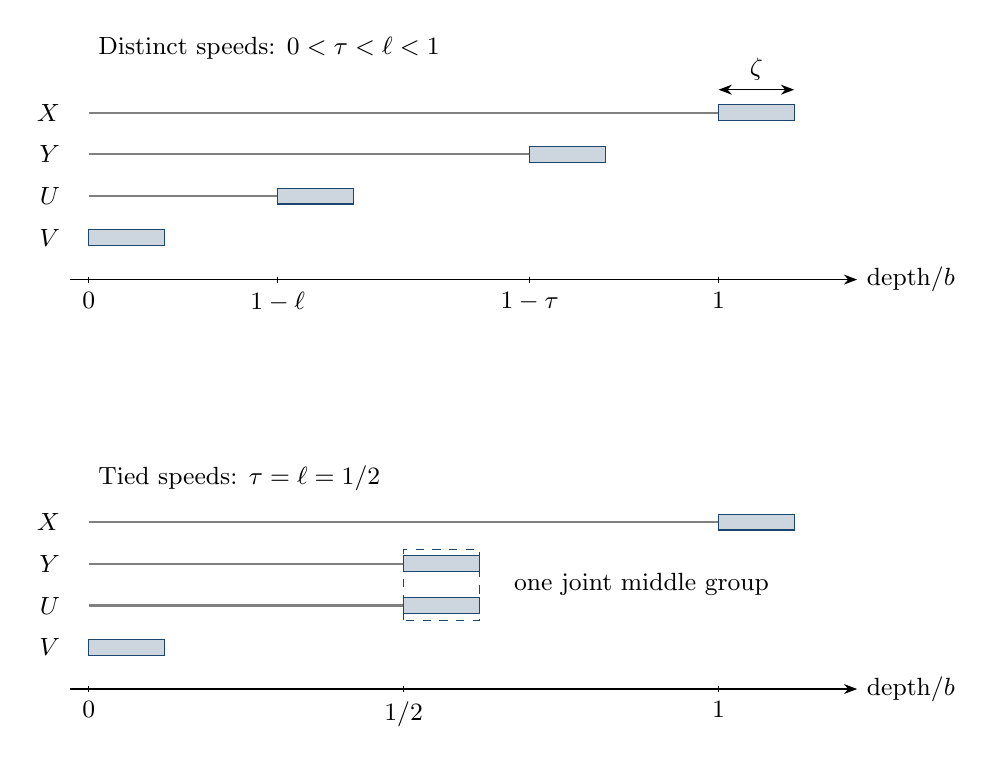
\begin{tikzpicture}[x=8.0cm,y=.53cm,>=Stealth,font=\small]
\draw[->] (-.03,0)--(1.22,0) node[right] {depth$/b$};
\foreach \x/\lab in {0/0,.3/{1-\ell},.7/{1-\tau},1/1}
 {\draw (\x,.07)--(\x,-.07) node[below] {$\lab$};}
\foreach \y/\name/\left in {1/V/0,2/U/.3,3/Y/.7,4/X/1}
 {\node[left] at (-.03,\y) {$\name$};
  \draw[gray,thick] (0,\y)--(\left,\y);
  \filldraw[fill=linkblue!22,draw=linkblue] (\left,\y-.19) rectangle +(0.12,.38);}
\draw[<->] (1,4.55)--(1.12,4.55) node[midway,above] {$\zeta$};
\node[anchor=west] at (0,5.55) {Distinct speeds: $0<\tau<\ell<1$};
\begin{scope}[yshift=-5.2cm]
\draw[->] (-.03,0)--(1.22,0) node[right] {depth$/b$};
\foreach \x/\lab in {0/0,.5/{1/2},1/1}
 {\draw (\x,.07)--(\x,-.07) node[below] {$\lab$};}
\foreach \y/\name/\left in {1/V/0,2/U/.5,3/Y/.5,4/X/1}
 {\node[left] at (-.03,\y) {$\name$};
  \draw[gray,thick] (0,\y)--(\left,\y);
  \filldraw[fill=linkblue!22,draw=linkblue] (\left,\y-.19) rectangle +(0.12,.38);}
\draw[dashed,linkblue] (.5,1.65) rectangle (.62,3.35);
\node[anchor=west] at (.66,2.5) {one joint middle group};
\node[anchor=west] at (0,5.05) {Tied speeds: $\tau=\ell=1/2$};
\end{scope}
\end{tikzpicture}
\caption{Schematic rebased coordinate windows for the local matrix
experiment in Section~\ref{sec:projections}. Gray segments show the base observations;
shaded windows show the additional refinements. Relative to the original offset, the base
of axis $i$ is shifted by $(1-k_i)b$, and its additional observation
has depth $\zeta b$. When $\zeta$ is smaller than every nonzero speed
separation, the windows of distinct groups are disjoint. At each window,
all groups with smaller $k_i$ are already observed in the full base
cell. The other distinct-speed order exchanges $Y$ and $U$.
Tied coordinates overlap and must retain their joint rate.}
\label{fig:entropy-layers}
\end{figure}


\begin{lemma}[Local counts and conditional Frostman laws]
\label{lem:blowup-counts}
There is a triangular choice $b_n\downarrow0$, $N_n\to\infty$,
with $D_n=N_n^{b_n}\to\infty$, and uniform refinements of the
single-event graphs, chosen independently of the queried offset,
with the following properties at almost every admissible offset
$a$. At stage $n$, evaluate the finite experiment at a prescribed
grid offset $a_n$ with $|a_n-a|=o(b_n)$; all rates below are
evaluated at the limiting point $(c,a)$. Conditional on
\[
 \mathcal B=(E_0,J_0,L),
\]
the entropy of $\mathcal O_{\mathbf u}$, divided by $\log D$, is
\begin{equation}
 \mathcal R(\mathbf u)+o(1).
\label{pr:local-entropy-formula}
\end{equation}
For distinct speeds,
\[
 \mathcal R(\mathbf u)=\sum_i j_i u_i.
\]
For tied middle speeds, put
\[
 r_Y=\phi_{\{X,Y\}}-\phi_{\{X\}},\qquad
 r_U=\phi_{\{X,U\}}-\phi_{\{X\}}.
\]
Then
\begin{equation}
 \mathcal R(\mathbf u)
   =a_1u_X+v_1u_V+
 \begin{cases}
    r_Y(u_Y-u_U)+m_1u_U,&u_Y\ge u_U,\\
    r_U(u_U-u_Y)+m_1u_Y,&u_U\ge u_Y.
 \end{cases}
\label{pr:tied-rectangle}
\end{equation}
These formulas hold for joint and unequal-depth observations.
Their occupied conditional cells have probabilities
\begin{equation}
 \Prob(\mathcal O_{\mathbf u}=o\mid\mathcal B)
      =D^{-\mathcal R(\mathbf u)+o(1)}
\label{pr:local-cell-masses}
\end{equation}
uniformly on the regularized graph at every tested depth.
Ratios of joint and conditioning cell probabilities give the
corresponding conditional formulas.

In particular, fix nuisance axes at relative depth $\zeta$ and
observe a selected pair to any depth $0\le u\le\zeta$.
For distinct speeds its conditional point law is Frostman of
exponent equal to the sum of the two selected rates, with subpower
constant, through resolution $D^{-\zeta}$.
For tied middle speeds, the additional $U$-rate after observing
$Y$ to depth $\zeta$ is $m_1-r_Y$; the pair $(X,V)$ after fixing
$Y,U$ has exponent $a_1+v_1$.

The same triangular choice supplies, conditionally on the original
index and $E_0$, the time and normal-parameter Frostman bounds of
exponents $s_0$ and $\gamma$ in relative units.
When $\tau=\ell$, the joint parameter square cells have masses
$D^{-s_0u+o(1)}$ for $0\le u\le\zeta_{\max}$.
\end{lemma}

\begin{proof}
We prove the rectangular entropy formula first. We then realize its
values as uniform finite cell masses and verify the time and normal
laws needed to choose a second event.

\paragraph{Rectangular entropy increments.}
Fix $\sigma>0$ and, temporarily, take $b$ so small that
$C_0b<\sigma$ and $c+\sigma<1$.
Condition additionally on $e_{c+\sigma}$ and read all forms in
that finer frame. Given $L$, Lemma~\ref{lem:pr-relative-frame}
shows that the required observations in the two frames determine
one another up to bounded overlaps. The full starting cell is
included in this comparison; errors from unobserved components
are below the finest tested width.

Apply the rectangular layering conclusion of
Lemma~\ref{lem:gap-density}. The starting offsets of the four
increment intervals are
\[
 a+(1-k_i)b.
\]
Intervals belonging to different speed groups are disjoint, because
$\zeta_{\max}<|k_i-k_j|$.
During the interval for a group of speed $k$, every group of smaller
speed has already been required to a depth beyond that interval,
even in its \emph{base} observation. Every group of larger speed
ends below the interval. If $S$ is the union of the groups of smaller
speed and $G$ is the current group, subtraction of the base rectangle from the refined
rectangle leaves the density
$\phi_{S\cup G}^{\sigma}-\phi_S^{\sigma}=:j_G^{\sigma}$.
Thus the group's contribution is its ordered conditional rate times
its refinement depth.
This reasoning applies both to the order $X,Y,U,V$, when
$\tau<\ell$, and to $X,U,Y,V$, when $\ell<\tau$.
It gives \eqref{pr:local-entropy-formula} with the
$\sigma$-conditioned rates, to error $o(b)$ in entropy divided by
$\log N$.

For a tied group, first reveal $Y$ and $U$ together to the smaller
of their two depths; then refine only the deeper coordinate. The
common part costs $m_1$ times that depth. The remaining
increment uses $r_Y$ or $r_U$, according to the deeper coordinate.
This gives \eqref{pr:tied-rectangle}, again first with
$\sigma$-conditioned rates.
Equivalently, one may subtract the layering formulas for a joint
rectangle and its conditioning rectangle. All their thresholds lie
within $a\pm Cb$ for a fixed $C$.

We next remove the extra label. Given $L$, the joint and
conditioning observations in question are sandwiched between full
$e_c$-frame observations at offsets $a-Cb$ and $a+Cb$, up to bounded
overlaps. By Lemma~\ref{lem:remove-label}, the change of a
conditional increment upon adding $e_{c+\sigma}$ is bounded by
the incremental label information on this full-cell interval.
For almost every $a$, its upper first-order density tends to zero
as $\sigma\downarrow0$.
Consequently the limsup of the error divided by $b$, as $b\to0$
with $\sigma$ fixed, is bounded by a constant times that density.
Now let $\sigma\downarrow0$ through a countable sequence.
The rates converge to $\phi_S$ and $j_G$, and the error is $o(b)$.
This proves the asserted formulas for the limiting normalized
entropies without requiring a convergence speed uniform in $a$.

\paragraph{Uniform finite cell masses.}
Here is a simultaneous implementation on finite configurations.
Fix a summable sequence of positive rational $b_n\downarrow0$.
At stage $n$, prescribe a finite offset grid of spacing $o(b_n)$
on the compact interval under consideration, and a finite grid of
relative depths whose union is dense in
$[0,\zeta_{\max}]$. Include the following in the countable family
of tests: $E_0,J_0,L$; every subset of the axis observations at
equal and unequal depths; their joint and conditioning cells;
the full-cell sandwiches just used; and the same observations with
the fixed additional labels $e_{c+\sigma}$.
Include also the within-index parameter-cell tests described below.

Use Lemma~\ref{lem:regularization} on finitely many tests at a time,
including the deficient-cell deletions relative to their original
mass. This makes the joint and conditional cell masses uniform in
exponent. Previously uniform tests keep their limits: surviving
cells retain their original masses within the prescribed subpower
factor, and the total restriction has the same order of loss.
Thus the already defined stable entropy function and its rates do
not change.
Take subsequential limits on this countable family first.
Their values satisfy the estimates established above with fixed
$\sigma$ and then $\sigma\downarrow0$.

Finally choose $N_n$ sufficiently large along the resulting
configurations that the first $n$ finite collections of tests have
errors $o(b_n)$ in exponents normalized by $\log N_n$.
The finite pigeonholings and cleaning can have total loss
$N_n^{-o(b_n)}$: for a fixed finite number of tests their number of
mass levels grows at most polynomially in $\log N_n$ and in the
inverse requested accuracy, so increasing $N_n$ makes their
normalized logarithmic cost smaller than the chosen multiple of
$b_n$. Choose the deletion cutoffs below that retention while still
with exponent $o(b_n)$.
Also require $b_n\log N_n\to\infty$.
For each generic $a$, use its nearest offset-grid point.
The stable full-cell and finer-label comparisons change the
exponents by $o(b_n)$ at this replacement.
The first-order density estimates hold at the actual generic point
for every sequence $b_n\to0$; no uniform differentiability rate
over all such points was used.

Uniform joint cell masses now prove
\eqref{pr:local-cell-masses}, rather than only its entropy average.
For example, in the tied case and $u\le\zeta$,
\begin{align*}
 &\mathrm H( U_u,Y_\zeta\mid\mathcal B)
       -\mathrm H(Y_\zeta\mid\mathcal B)\\
 &\hspace{25mm}=(m_1-r_Y)u\log D+o(\log D).
\end{align*}
The probability of an occupied $U_u$ cell within an occupied
$Y_\zeta$ cell is the ratio of their joint and marginal
probabilities, hence $D^{-(m_1-r_Y)u+o(1)}$.
For distinct speeds the same subtraction removes all nuisance
terms and leaves $u$ times the sum of the selected rates.
For $(X,V)$ with $Y,U$ fixed, the tied-group contribution cancels
and leaves $(a_1+v_1)u$.
These statements hold at all the tested intermediate depths.
Bounded square coverings and increasingly fine depth meshes give
the asserted Frostman upper bounds at every intermediate radius.

\paragraph{Time and normal parameters.}
It remains to verify the parameter hypotheses for these finite
experiments. Lemma~\ref{lem:angular-frostman} and the uniform time
branching give the two upper bounds conditional on the index and
$E_0$. Nondeficient $E_0$ cells have the same exponent as their
time blocks, since each index uses only subpower many angular bins
there. Add these conditional cells and their refinements to the
tests before choosing the triangular sequence.
When $\tau=\ell$, refining the label from $c+b$ to
$c+b+ub/\ell$ multiplies both relative widths by $D^{-u}$.
The time mass is $D^{-s_0u+o(1)}$. Within each of its time blocks,
the normal range occupies only subpower many corresponding
angular bins. Its nondeficient occupied joint cells therefore have
that same mass exponent. Cleaning them gives the lower as well as
the upper bound, uniformly through the required depths.
All of this cleaning precedes the choice of a pair law; a later
bias is never applied to an uncontrolled exceptional set of
single-event cells.
\end{proof}

\subsection{The product-slope pinning input}

When $\tau=\ell$, the local count formula supplies the joint middle
rate $m_1$, rather than two separate ordered middle rates. To bound
$v_1$ in this case, freeze both $Y$ and $U$ in the first formula of
\eqref{pr:relative-frame}. The remaining projection is
\[
 X'=X+(\Delta t\Delta\vartheta)V
                    +\Delta t\,U+\Delta\vartheta\,Y.
\]
The last two terms are a translation once the nuisance coordinates
and the two labels are fixed. The slope is the product of two
parameter differences; their separate Frostman bounds do not assert
that this product is nonconcentrated. The following lemma supplies
that bound while controlling the change in each single-event law.

In its statement $D\to\infty$ is a resolution parameter and $\zeta$
is a positive depth. Neither denotes a critical parameter.
A probability $\mu$ on a bounded square is called uniformly
$s$-regular through depth $\zeta_{\max}$ if, for every occupied
nested dyadic square $Q$ of side comparable to $D^{-u}$,
\begin{equation}
 D^{-su-\epsilon_D}\le\mu(Q)\le D^{-su+\epsilon_D},
 \qquad 0\le u\le\zeta_{\max},\qquad \epsilon_D\longrightarrow0.
\label{pr:square-regularity}
\end{equation}
Fixed factors from dyadic rounding can be included in
$D^{\epsilon_D}$. It is equivalent here to impose these estimates
on depth meshes whose spacing tends to zero: monotonicity gives
\eqref{pr:square-regularity}, with a slightly larger error.
Uniformity for an ensemble means that the same error works for all
its members after deleting a set of initial indices of probability
tending to zero.

\begin{lemma}[Pinning with controlled marginals]
\label{lem:pinning}
Let $0<s\le1$, $\gamma'>0$, and $0<\zeta_{\max}\le1$ be fixed.
For each $D$, let $I$ have a finite probability distribution $\pi_D$,
and let $\mu_i$ be finitely supported probabilities on a fixed
bounded square with coordinates $(t,\vartheta)$.
Suppose uniformly in $i$ that \eqref{pr:square-regularity} holds and
that the two coordinate marginals satisfy
\begin{equation}
 \mu_i\{t\in J_r\}\le D^{o(1)}r^s,
 \qquad
 \mu_i\{\vartheta\in J_r\}\le D^{o(1)}r^{\gamma'}
 \quad(D^{-\zeta_{\max}}\le r\le1)
\label{pr:coordinate-frostman}
\end{equation}
for all intervals $J_r$ of radius $r$.
For every $\epsilon>0$, there are a subsequence, a fixed rational
$\zeta\in(0,\zeta_{\max}]$, and a probability $\nu_D$ on triples
$(i,\xi,\upsilon)$, with $\xi,\upsilon\in\supp\mu_i$, such that:
\begin{enumerate}[label=\textup{(\roman*)}]
\item each marginal $(i,\xi)$ and $(i,\upsilon)$ is dominated by
$D^{\epsilon\zeta}\pi_D(di)\mu_i$;
\item for $\nu_D$-almost every $(i,\xi)$, the conditional law of
\[
 \mathfrak p_\xi(\upsilon)
   =(t_\upsilon-t_\xi)(\vartheta_\upsilon-\vartheta_\xi)
\]
satisfies
\begin{equation}
 \nu_D\{\mathfrak p_\xi(\upsilon)\in J_r\mid i,\xi\}
 \le C D^{\epsilon\zeta}r^{s-\epsilon},
 \qquad D^{-\zeta}\le r\le1.
\label{pr:pinned-frostman}
\end{equation}
\end{enumerate}
The pair law can be chosen using only the initial index and its
parameter measure. In particular it need not depend on any later
matrix-cell or offset test.
\end{lemma}

The proof of Lemma~\ref{lem:pinning} is in
Section~\ref{sec:product-pinning-proof}.

\subsection{Two events on one index}

Let $\mu$ be the probability on the regularized single-event graph.
First draw $(I,E_0)$ from its marginal under $\mu$. For the
\emph{ordinary pair law}, draw $\xi_0,\xi_1$ conditionally
independently from the original law given $(I,E_0)$. Both events use
the matrix attached to $I$. Their conditional independence does not
make that matrix independent of their frame labels.
Let $L_0,L_1$ be their labels at the precision in
\eqref{pr:fine-label}.
Conditional on $(I,E_0,\xi_0)$, the difference of the second time
from the first is $s_0$-Frostman, and the corresponding normal
difference is $\gamma$-Frostman, in relative units. Translation
does not change either estimate. Reading the differences from
$L_0,L_1$ changes them by less than the testing resolution, by
Lemma~\ref{lem:pr-relative-frame}. Bounded enlargement of intervals
therefore preserves their Frostman bounds.

In the tied case we need one additional coupling. Apply
Lemma~\ref{lem:pinning} to the within-index parameter laws given
$(I,E_0)$, with $s=s_0$, using the last assertion of
Lemma~\ref{lem:blowup-counts}. For any fixed sufficiently small
$\epsilon>0$, it gives, along a further subsequence, a fixed
rational depth $\zeta>0$. Both single-event marginals are bounded
by $D^{\epsilon\zeta}$ times their original laws. Conditional on
$(I,E_0,\xi_0)$ the product slope
\begin{equation}
 \Theta_*=(t_1-t_0)(\vartheta_1-\vartheta_0)
\label{pr:product-slope}
\end{equation}
is $(s_0-\epsilon)$-Frostman with constant
$CD^{\epsilon\zeta}$ through resolution $D^{-\zeta}$.
All coordinates here are in the relative parameter units of
$E_0$. The product is Lipschitz on this fixed bounded square, so
the fine-label replacement preserves this estimate as well.

The original graph and these pair distributions are chosen before
querying an offset. We can prescribe countably many loss
tolerances and projection tests. Each can use a further subsequence;
intersecting their resulting full-measure sets of offsets still
gives a full-measure set. No one choice of pair distribution is
asserted to work for every tolerance.

The same-index relation forces the matrix, read in the second frame,
to belong to the support of that frame's original coordinate law. We
will compare this certain event with its probability under the product
of the conditional matrix and label marginals. A small probability
under that product would require positive mutual information. The
next estimate shows that the short matrix-refinement gap contains
asymptotically less information than such a comparison would require.
It applies equally to the ordinary and pinned pair laws. The finite
pair law may depend on $b,N,I,E_0$, but it must be fixed while the offset
is integrated.

\begin{lemma}[Pair information on the refinement gap]
\label{lem:pair-information}
Let $K=1+\zeta_{\max}$, and let $J_f$ be the full observation in
the $E_0$-frame obtained by increasing every threshold of $J_0$
by $Kb$. Along a triangular subsequence as in
Lemma~\ref{lem:blowup-counts}, for almost every admissible offset,
\begin{equation}
 \mathrm I(J_f;L_0,L_1\mid E_0,J_0)=o(\log D).
\label{pr:pair-information}
\end{equation}
Here $J_0,J_f$ are evaluated at the nearest prescribed offset-grid
point. The assertion holds for every one of the countably many
pair experiments just described, with ordinary Shannon units.
\end{lemma}

\begin{proof}
Given $E_0$, each label $L_i$ has at most
$C N^{C_1b}$ possible values, where $C_1$ depends on $C_0$ and
the fixed speeds. This is an alphabet bound from the time and
normal grids, independent of the probabilities of these labels.
It remains true under either marginal bias. Consequently
\begin{equation}
 \mathrm H(L_0,L_1\mid E_0)\le C_2(1+b\log N).
\label{pr:label-alphabet}
\end{equation}

Temporarily write $J_0(a)$ for the rebase grid at offset $a$ and
set
\[
 f(a)=\mathrm I(J_0(a);L_0,L_1\mid E_0).
\]
This is nondecreasing, because the matrix grids are nested as $a$
increases. Its range is contained in
$[0,C_2(1+b\log N)]$. The chain rule gives the exact identity
\begin{equation}
 f(a+Kb)-f(a)
 =\mathrm I(J_0(a+Kb);L_0,L_1\mid E_0,J_0(a)).
\label{pr:information-increment}
\end{equation}
For a nondecreasing function with range of length $H_*$,
\[
 \int_A^B[f(a+q)-f(a)]\,da\le qH_*
 \qquad(q>0),
\]
as follows either by changing variables in the two integrals or
by integrating its nonnegative increment measure.
For a grid replacement $a_n$ with $|a_n-a|=o(b_n)$, monotonicity
also bounds the left side of \eqref{pr:information-increment}
by
\[
 f(a+(K+1)b)-f(a-b)
\]
for large $n$. Integrate on a compact interval whose slightly
larger neighborhood stays admissible. Equations
\eqref{pr:label-alphabet} and \eqref{pr:information-increment}
give
\begin{equation}
 \int
 \frac{\mathrm I(J_f;L_0,L_1\mid E_0,J_0)}{\log D}\,da
 \le C_3\left(b+\frac1{\log N}\right).
\label{pr:information-integral}
\end{equation}
The left side uses the stepwise chosen grid offsets. The
containing-gap estimate proves the bound regardless of the sizes
of the grid's inverse images.

Choose $b_n$ summable, and increase $N_n$ so that
$1/\log N_n$ is summable as well as satisfying all the finite
tests of Lemma~\ref{lem:blowup-counts}. Tonelli's theorem applied
to the nonnegative functions in
\eqref{pr:information-integral} shows that their sum is finite
almost everywhere. In particular the summands tend to zero,
which proves \eqref{pr:pair-information}.
A further subsequence, such as the one used for pinning, preserves
this conclusion. For countably many pair experiments use the same
integral argument for each and intersect the full-measure sets.
Finally exhaust the admissible offset domain by compact intervals.
\end{proof}

We next record explicitly how the marginal bias is used. Denote
the first single-event marginal of a chosen pair law by $\nu$.
Suppose
\begin{equation}
 \nu\le D^{\epsilon\zeta}\mu.
\label{pr:marginal-domination}
\end{equation}
Let $\mathcal B_0=(E_0,J_0,L_0)$.
Discard base values $B$ for which
$\nu(B)<D^{-\epsilon\zeta}\mu(B)$.
Their total $\nu$-probability is at most $D^{-\epsilon\zeta}$.
For every other base, division of
\eqref{pr:marginal-domination} by its base mass gives
\begin{equation}
 \nu(\,\cdot\mid B)
       \le D^{2\epsilon\zeta}\mu(\,\cdot\mid B).
\label{pr:conditional-domination}
\end{equation}
This also holds for the conditional matrix marginals.
For the ordinary pair law the first marginal equals
$\mu$, and no base deletion is needed.

\subsection{Comparing the coupling with a product law}

For a fixed base $B=(E_0,J_0,L_0)$, the actual pair experiment
defines a joint law of the matrix and $L_1$.
The conditional slope law is obtained by mixing its laws given
$(I,E_0,\xi_0)$. Since $J_0$ is determined by the matrix and
$E_0$, this conditioning and mixture preserve each of the uniform
time, angular, or pinned-product Frostman bounds above.
We compare the joint law with the product of its two conditional
marginals. Independence is imposed only in this comparison law.

The planar estimate we use keeps the entire direction label: two
labels with the same slope may prescribe different target intervals.
Its point and label measures are independent in the product below.
The proof is given in Section~\ref{sec:robust-projection-proof}.

\begin{lemma}[Robust planar projections]\label{lem:robust-projection}
Fix
\[
 0<s\le1,\qquad 0<t\le2,\qquad
 0\le u<h_{\mathrm{pr}}:=\min\{t,(s+t)/2,1\}.
\]
There is $\kappa_0=\kappa_0(s,t,u)>0$ with the following property.
For every $R,C_0\ge1$ and $0<\kappa\le\kappa_0$, there is
$\delta_0>0$ such that the following holds for
$0<\delta<\delta_0$. Let $\mu$ be a Borel subprobability measure
on $[-R,R]^2$, let $\nu$ be a subprobability measure on an
arbitrary finite label set $\Lambda$, and let
$\vartheta:\Lambda\to[-R,R]$. Suppose
\begin{equation}\label{eq:robust-projection-frostman}
 \mu(B(p,r))\le\delta^{-\kappa}r^t,
 \qquad
 (\vartheta_*\nu)(B(a,r))\le\delta^{-\kappa}r^s
 \quad(\delta\le r\le1).
\end{equation}
For each $\lambda\in\Lambda$, let $A_\lambda$ be a union of at
most $C_0\delta^{-u}$ intervals of length at most $C_0\delta$.
Then
\begin{equation}\label{eq:robust-projection-product}
 \sum_{\lambda\in\Lambda}\nu(\{\lambda\})
 \mu\{(x,y):x+\vartheta(\lambda)y\in A_\lambda\}
 <\delta^{2\kappa}.
\end{equation}
Consequently there cannot be a set $B\subset\Lambda$ with
$\nu(B)\ge\delta^\kappa$ such that for every $\lambda\in B$
there is a $\mu$-measurable set $E_\lambda$ with
\begin{equation}\label{eq:robust-projection-subset}
 \mu(E_\lambda)\ge\delta^\kappa,
 \qquad
 \{x+\vartheta(\lambda)y:(x,y)\in E_\lambda\}
 \subset A_\lambda.
\end{equation}
\end{lemma}

\begin{lemma}[Transfer of a projection bound to rates]
\label{lem:pr-projection-transfer}
Fix the original single-event law $\mu$ and one of the same-index
pair laws above, with the conditional marginal domination already
established. Suppose that after freezing
the nuisance axes at relative depth $\zeta$, the original
conditional law of two source coordinates is Frostman with
exponent $t>0$ and subpower constant through resolution
$\delta=D^{-\zeta}$, uniformly in its occupied nuisance fibers.
Suppose that, in the pair law conditional on $B$, the changing
projection slope has an available positive Frostman exponent $s\le1$.
In a pinned experiment, ``available'' means exponents tending to
$s$ with arbitrarily small fixed marginal and Frostman losses.
Suppose further that the target coordinate in the $L_1$-frame
has, conditional on $(E_0,J_0,L_1)$, at most
$D^{a_*\zeta+o(1)}$ occupied bins of width comparable to
$D^{-\zeta}$.
Then
\begin{equation}
 a_*\ge \min\{t,(t+s)/2,1\}.
\label{pr:projection-transfer}
\end{equation}
\end{lemma}

\begin{proof}
Suppose the inequality fails strictly. Choose fixed
$0<t_*<t$, $0<s_*<s$, and $u>a_*$, still satisfying
\begin{equation}
 u<\min\{t_*,(t_*+s_*)/2,1\}.
\label{pr:strict-projection-margin}
\end{equation}
The choices are possible by continuity, and are made before any
pinning loss is chosen. Let $\kappa>0$ be an allowance from
Lemma~\ref{lem:robust-projection} for these three fixed exponents.
In the pinned case choose the loss tolerance $\epsilon$ so small
that
\begin{equation}
 \epsilon<s-s_*,\qquad 2\epsilon<\kappa/2.
\label{pr:loss-order}
\end{equation}
Choose the pinned coupling and its fixed positive depth $\zeta$
with this tolerance. For the ordinary pair law any fixed rational
$0<\zeta\le\zeta_{\max}$ works. The depth does not subsequently
shrink with $D$. Subpower errors in the original single-event
estimates therefore tend to zero also after division by $\zeta$.

\paragraph{The product probability bound.}
Fix a good base $B$, and initially use the \emph{original}
conditional matrix law $\mu(\,\cdot\mid B)$, independently of
the pair experiment's conditional law of $L_1$.
Within this original matrix law, freeze the nuisance bins at
depth $\zeta$. Lemma~\ref{lem:blowup-counts} gives the point
Frostman bounds, with exponent $t_*$, in every occupied fiber.
For sufficiently large $D$ their constants are smaller than
$\delta^{-\kappa}$. The slope bounds, with exponent $s_*$, have
the same allowed constant: in the pinned case they cost
$C\delta^{-\epsilon}$, and for the ordinary pair law a subpower.

The frame formula \eqref{pr:relative-frame} writes the target
coordinate as a two-coordinate scalar projection plus a
translation depending on the frozen nuisance bins and the full
label $L_1$. The error from a nuisance bin has size $O(\delta)$,
since all coefficients are bounded. For each $L_1$, enlarge all
its allowable target bins by this error and subtract the known
translation. Their number is at most $C\delta^{-u}$, because
$u>a_*$. Their lengths are at most $C\delta$.
The label may contain more information than the projection slope;
Lemma~\ref{lem:robust-projection} permits precisely this dependence
of the target intervals on the entire label.

Apply that lemma in each original nuisance fiber, with fixed
bounded coordinate charts. Its independent product hit
probability is less than $\delta^{2\kappa}$, uniformly in the
fiber. Integrating over the original nuisance distribution gives
the same bound for the entire original conditional matrix law.
Only now replace that whole matrix law by its biased marginal.
Equation~\eqref{pr:conditional-domination} bounds the new product
hit probability by
\begin{equation}
 \delta^{-2\epsilon}\delta^{2\kappa}
       \le\delta^{\kappa}
\label{pr:biased-product-hit}
\end{equation}
for large $D$. For the ordinary pair law the domination factor is
one. This argument does not assume that biased nuisance fibers
have the original Frostman estimates, or that a slope remains
independent after conditioning inside the actual coupling.

\paragraph{The support event for the same-index law.}
Under the true coupling, the target matrix coordinate always
belongs to the allowed support for $(E_0,J_0,L_1)$.
Both pair marginals are supported on the original single-event
graph and both events have exactly the same index matrix. Thus
this support test has probability one in the true coupling.
It requires no probability lower bound for target cells after
the change of measure.

To make it a finite information test, replace the matrix by a
representative of its $J_f$ cell. The relative coordinate error
is $O(D^{-(1+\zeta_{\max})})$, which is smaller than
$D^{-\zeta}$ by a fixed positive power. The bounded frame
coefficients and the precision of $L_0,L_1$ leave an
$O(\delta)$ error. Enlarge the target bins once more.
The resulting event $A_B$ depends only on $(J_f,L_1)$ at fixed
$B$, has conditional probability one in the true coupling, and
still has probability at most $\delta^\kappa$ under the product
of the conditional marginals of $J_f$ and $L_1$.
For the last assertion, sample the exact matrix from its
conditional marginal and then round it. A rounded hit implies
an exact hit in one further bounded enlargement, already allowed
in the preceding application of Lemma~\ref{lem:robust-projection}.

\paragraph{The information contradiction.}
Let $P_B$ be the conditional joint law of $(J_f,L_1)$ and $Q_B$
the product of its marginals. Data processing of relative entropy
by the indicator of $A_B$ gives
\[
 \mathrm I(J_f;L_1\mid B)
   =\mathrm D_{\mathrm{KL}}(P_B\Vert Q_B)
   \ge \log\frac1{Q_B(A_B)}
   \ge \kappa\zeta\log D.
\]
The good bases have pair probability tending to one by
\eqref{pr:conditional-domination}. Averaging the last inequality
therefore gives
\begin{equation}
 \mathrm I(J_f;L_1\mid E_0,J_0,L_0)
   \ge (1-o(1))\kappa\zeta\log D.
\label{pr:information-contradiction}
\end{equation}
On the other hand the chain rule and nonnegativity imply
\[
 \mathrm I(J_f;L_1\mid E_0,J_0,L_0)
 \le \mathrm I(J_f;L_0,L_1\mid E_0,J_0)
 =o(\log D)
\]
by Lemma~\ref{lem:pair-information}. Since $\kappa\zeta>0$
is fixed, this contradicts
\eqref{pr:information-contradiction} and proves the lemma.
\end{proof}

\subsection{Deriving the individual constraints}

\begin{proof}[Proof of Proposition~\ref{prop:projection-rates}]
Fix a good interior $c$. Work at offsets where the entropy
densities, the local counts, and the pair information conclusions
all hold. Strict violations of any inequality can be witnessed
by rational choices of the smaller exponents and loss tolerances
in \eqref{pr:strict-projection-margin}--\eqref{pr:loss-order}.
There are countably many such choices, so the preceding
constructions apply on a common full-measure set of offsets.
Fubini then gives the asserted almost-everywhere statement in
$(c,a)$.

For distinct speeds the four tests needed below are displayed in
Table~\ref{tab:pr-tests}. Each uses the ordinary pair law. Source
exponents are conditional on the listed
nuisance bins in the original matrix law. They follow from the
all-depth probability ratios in Lemma~\ref{lem:blowup-counts},
in either of the two possible speed orders.

\begin{table}[htbp]
\centering
\small
\begin{tabular}{@{}llllll@{}}
\toprule
Target & Source pair & Frozen axes & Slope & Source exponent
 & Target exponent\\
\midrule
$X$ & $(X,Y)$ & $U,V$ & $\Delta\vartheta$ & $a_1+y_1$ & $a_1$\\
$X$ & $(X,U)$ & $Y,V$ & $\Delta t$ & $a_1+u_1$ & $a_1$\\
$U$ & $(U,V)$ & $X,Y$ & $\Delta\vartheta$ & $u_1+v_1$ & $u_1$\\
$Y$ & $(Y,V)$ & $X,U$ & $\Delta t$ & $y_1+v_1$ & $y_1$\\
\bottomrule
\end{tabular}
\caption{The four ordinary-pair tests for distinct speeds.
The angular and time slope exponents are respectively
$\gamma$ and $s_0$.}
\label{tab:pr-tests}
\end{table}

For example the first formula of
\eqref{pr:relative-frame}, with $U,V$ frozen, is
\[
 X'=X+\Delta\vartheta Y
       +\Delta t U+\Delta t\Delta\vartheta V.
\]
The last two terms are a full-label-dependent translation up to
$O(D^{-\zeta})$. With $Y,V$ frozen, the same expression is
$X+\Delta t U$ plus such a translation. The second and third
formulas give the other two rows. Thus every row has exactly the
form required in Lemma~\ref{lem:pr-projection-transfer}.

It is useful to spell out the numerical implication. For
$0\le a,b\le1$ and $s>0$, suppose the test with source exponent
$a+b>0$ gives
\begin{equation}
 a\ge\min\{a+b,(a+b+s)/2,1\}.
\label{pr:elementary-test}
\end{equation}
If $a<1$ and $b>0$, both the first and the third entries of this
minimum exceed $a$. The second must therefore be at most $a$,
so $b\le a-s$. If $b=0$ there is no further restriction.
In either case
\begin{equation}
 a<1\quad\Longrightarrow\quad b\le(a-s)_+.
\label{pr:elementary-consequence}
\end{equation}
When $a+b=0$, that conclusion is immediate without applying the
projection lemma.

The first row gives $y_1\le(a_1-\gamma)_+$ when $a_1<1$.
Together with $y_1\le1$, this implies $a_1\ge y_1$ also when
$a_1=1$. The second row gives
$u_1\le(a_1-s_0)_+$ whenever $a_1<1$.
The third row analogously gives $u_1\ge v_1$.
For the last row, if $v_1>0$ and $y_1<1$,
\eqref{pr:elementary-consequence} gives $y_1\ge s_0+v_1$.
If $y_1=1$, the required
$y_1\ge\min\{1,s_0+v_1\}$ holds automatically.
These are all assertions of \eqref{pr:distinct-constraints}.

Suppose now that $\tau=\ell$. Put
\[
 r_Y=\phi_{\{X,Y\}}-\phi_{\{X\}}.
\]
Conditional entropy monotonicity and the one-dimensional
alphabet bound give
$0\le r_Y\le1$ and $0\le m_1-r_Y\le1$.
Use the second row's time projection with $Y,V$ frozen.
For every $0\le u\le\zeta$, the tied rectangle formula gives
the conditional source exponent
\[
 t=a_1+(m_1-r_Y).
\]
The target exponent is $a_1$ and the slope exponent is $s_0$.
Equation~\eqref{pr:elementary-consequence}, with
$b=m_1-r_Y$, yields
\[
 a_1<1\quad\Longrightarrow\quad
 m_1-r_Y\le(a_1-s_0)_+.
\]
Since $r_Y\le1$, this proves the bound for $m_1$ in
\eqref{pr:tied-constraints}.

Finally freeze $Y,U$ and use the pinned pair distribution.
The first formula in \eqref{pr:relative-frame} becomes
\[
 X'=X+(\Delta t\Delta\vartheta)V
                 +\Delta t U+\Delta\vartheta Y.
\]
The source pair is $(X,V)$, of conditional exponent
$a_1+v_1$, by Lemma~\ref{lem:blowup-counts}.
Its target exponent is $a_1$.
The product slope has available exponent $s_0$ by
Lemma~\ref{lem:pinning} and the preceding coupling construction.
Lemma~\ref{lem:pr-projection-transfer} includes both its marginal
bias and its small direction loss. Thus
\eqref{pr:elementary-consequence} gives
$v_1\le(a_1-s_0)_+$ when $a_1<1$, as required.

Every construction above takes place on a compact subset of
$\mathcal U$ from \eqref{eq:entropy-domain}.
Indeed the smallest and largest of the four unshifted thresholds
are respectively
\[
 (1-w)(1-c)+a,\qquad 1-w(1-c)+a.
\]
If $w<1$, a compact interior $c$-interval admits sufficiently
small offsets of either sign, and the $O(b)$ rebase and
refinement shifts stay in range. If $w=1$, only positive small
offsets are interior. This proves the stated conclusion for every
permitted sign and completes the proposition.
\end{proof}

\section{Planar projection and product-pinning proofs}
\label{sec:projection-proofs}

This section proves the two planar statements used in
Section~\ref{sec:projections}. We first derive the robust projection
bound from the quantitative Furstenberg theorem. We then use that bound
to construct the pair law whose product slope is nonconcentrated.

\subsection{The robust projection bound}
\label{sec:robust-projection-proof}

We prove Lemma~\ref{lem:robust-projection}. Its parameters $s,t,u$
are fixed, and $h_{\mathrm{pr}}=\min\{t,(s+t)/2,1\}$ is the planar
projection exponent. A positive product hit probability would
produce a Furstenberg configuration with too few tubes: comparable
slope masses and incidence counts give the required quantitative
point and direction bounds.

\begin{proof}
Put $\Delta=h_{\mathrm{pr}}-u>0$ and $\varepsilon=\Delta/4$. Let
$\eta_{\mathrm{pr}}=\eta_{\mathrm{pr}}(\varepsilon,s,t)>0$ be the Frostman tolerance in
\citet[Theorem~4.1]{RW2025}. We may take
\begin{equation}\label{eq:robust-projection-kappa}
 \kappa_0=\min\{1/20,\Delta/16,\eta_{\mathrm{pr}}/12\}.
\end{equation}
All constants below may depend on $R,C_0,s,t$, but not on the
number of labels or on their weights. We decrease $\delta_0$
finitely many times.

First put the incidences in the bounded coordinates used for
dyadic tubes. Set $B_0=R+1$ and
\[
 v=\frac{y+B_0}{2B_0},\qquad
 w=\frac{x+B_0}{2B_0^2},\qquad
 a_\lambda=-\frac{\vartheta(\lambda)}{B_0}.
\]
Then $(v,w)\in(0,1)^2$, $a_\lambda\in(-1,1)$, and
\[
 w-a_\lambda v
 =\frac{x+\vartheta(\lambda)y+B_0(1+\vartheta(\lambda))}
        {2B_0^2}.
\]
Apply this affine transformation to $A_\lambda$, writing the
result as $J_\lambda$. Each $J_\lambda$ has at most
$C\delta^{-u}$ constituent intervals of length at most $C\delta$.
The transformed point and slope measures satisfy
\eqref{eq:robust-projection-frostman} with an additional fixed
factor $C$. We keep the notation $\mu$ for the transformed point
measure.

Choose a dyadic number $\varrho$ with
$\delta\le\varrho<2\delta$, and put
\[
 L=8\lceil\log_2(1/\delta)\rceil+8,
 \qquad q_*=\delta^{2\kappa}.
\]
Suppose that the left side of \eqref{eq:robust-projection-product}
is at least $q_*$. Write
$f(\lambda)=\mu\{(v,w):w-a_\lambda v\in J_\lambda\}$.
Partition the slopes into dyadic $\varrho$-intervals $I$. Give
$I$ its total label weight
$W_I=\nu\{\lambda:a_\lambda\in I\}$, and choose a label
$\lambda_I$ maximizing $f$ in that interval. There are finitely
many labels, so
\begin{equation}\label{eq:robust-projection-aggregate}
 \sum_I W_If(\lambda_I)\ge q_*.
\end{equation}
There are at most $C\delta^{-1}$ occupied slope intervals.
Discarding those with $W_I<\delta^4$ loses at most
$C\delta^3\le q_*/2$ from \eqref{eq:robust-projection-aggregate}.
The remaining weights have at most $L$ dyadic levels. One level,
consisting of $n$ slope intervals, satisfies
\[
 H_*:=\sum_{I\text{ in the level}}W_If(\lambda_I)
 \ge\frac{q_*}{2L}.
\]
Let $a_* =\sum_I W_I$ on this level. Its weights are within a
factor of two, and $H_*\le a_*\le1$. Consequently the uniform
distribution of its slope intervals satisfies
\begin{equation}\label{eq:robust-projection-slopes}
 \frac{\#\{I:I\cap B(b,r)\ne\varnothing\}}n
 \le CL\delta^{-3\kappa}r^s
 \quad(\varrho\le r\le1).
\end{equation}
Indeed, relative counting costs at most $2/a_*$ times the
original slope mass of a fixed enlargement of the ball, and
$a_*\ge q_*/(2L)$. For enlarged radii exceeding one, the same
bound follows from the total mass bound.

Let $d(p)$ be the number of selected representative tests
satisfied by $p=(v,w)$. Comparability of the slope weights gives
\[
 \int\frac{d(p)}n\,d\mu(p)
 \ge\frac{H_*}{2a_*}\ge\frac{q_*}{4L}.
\]
Since $0\le d(p)/n\le1$ and $\mu(\R^2)\le1$, the set
$G_0=\{p:d(p)\ge q_*n/(8L)\}$ has mass at least $q_*/(8L)$.
Pigeonhole its positive integer degrees into at most $L$
dyadic levels. This gives a Borel set $G\subset G_0$ and an
integer $M\ge1$ such that
\begin{equation}\label{eq:robust-projection-degrees}
 \mu(G)\ge\frac{q_*}{8L^2},\qquad
 M\le d(p)<2M\ (p\in G),\qquad
 M\ge\frac{q_*n}{16L}.
\end{equation}

Partition the point square into dyadic $\varrho$-squares and give
$Q$ the weight $\mu(G\cap Q)$. There are at most
$C\delta^{-2}$ squares. Discard weights below $\delta^4$; their
total is at most $C\delta^2\le q_*/(16L^2)$. A dyadic weight
pigeonhole gives a family $\mathcal P$ of squares with comparable
weights and total retained mass
\begin{equation}\label{eq:robust-projection-point-mass}
 b_*\ge\frac{q_*}{16L^3}.
\end{equation}
For each $Q\in\mathcal P$ choose $p_Q\in G\cap Q$.
Comparison between counting and these comparable cell weights
shows that $\mathcal P$ has relative $t$-Frostman constant
\begin{equation}\label{eq:robust-projection-point-constant}
 CL^3\delta^{-3\kappa}
\end{equation}
down to $\varrho$: passage to relative counts costs at most
$2/b_*$, and the original measure bounds the mass of a fixed
enlargement of each testing ball.

Here a dyadic $\varrho$-tube is the union of lines
$w=av+b$ with $(a,b)$ in a fixed dyadic parameter square of side
$\varrho$. For each selected slope representative $a_I$ and each
$b'\in J_{\lambda_I}$, include the tube whose parameter square
contains $(a_I,b')$. Call the resulting family $\mathcal T$.
Every $J_{\lambda_I}$ meets at most $C\delta^{-u}$ intercept
intervals, so
\begin{equation}\label{eq:robust-projection-tube-upper}
 |\mathcal T|\le Cn\delta^{-u}.
\end{equation}
For $Q\in\mathcal P$ and each representative test satisfied by
$p_Q=(v_Q,w_Q)$, select the tube with parameter cell containing
$(a_I,w_Q-a_Iv_Q)$. This tube intersects $Q$. Different slope
cells give different tubes. Denote this fiber by $\mathcal T(Q)$;
then $M\le|\mathcal T(Q)|<2M$.

A ball of radius $r$ in tube-parameter space restricts its slope
coordinate to an interval of comparable radius. By
\eqref{eq:robust-projection-slopes} and
\eqref{eq:robust-projection-degrees},
\begin{equation}\label{eq:robust-projection-fiber-constant}
 \frac{\#\{\text{parameter cells of }\mathcal T(Q)
                     \text{ meeting }B(z,r)\}}
      {|\mathcal T(Q)|}
 \le CL^2\delta^{-5\kappa}r^s
 \quad(\varrho\le r\le1).
\end{equation}
Thus the base cells and selected incident fibers form exactly
the quantitative configuration of
\citet[Definition~3.1 and Theorem~4.1]{RW2025}. The selected fiber
cardinalities lie between $M$ and $2M$, as
permitted by the cited theorem. For sufficiently small $\delta$, the
constants in \eqref{eq:robust-projection-point-constant} and
\eqref{eq:robust-projection-fiber-constant} are at most
$\varrho^{-\eta_{\mathrm{pr}}}$. In detail, arrange $CL^3\le\delta^{-\kappa}$
and use $6\kappa\le\eta_{\mathrm{pr}}/2$ together with
$\varrho<2\delta$.

The cited theorem now gives
\[
 |\mathcal T|\ge c_\varepsilon M\varrho^{-h_{\mathrm{pr}}+\varepsilon}
 \ge\frac{c'_\varepsilon}{16L}
             n\delta^{-h_{\mathrm{pr}}+\varepsilon+2\kappa}.
\]
Combining this with \eqref{eq:robust-projection-tube-upper} yields
\[
 1\ge\frac{c''_\varepsilon}{L}
             \delta^{-(\Delta-\varepsilon-2\kappa)}.
\]
But \eqref{eq:robust-projection-kappa} implies
$\Delta-\varepsilon-2\kappa\ge5\Delta/8>0$, so the right
side tends to infinity. This proves
\eqref{eq:robust-projection-product}.
Finally, \eqref{eq:robust-projection-subset} would make the product
hit probability at least $\nu(B)\delta^\kappa\ge\delta^{2\kappa}$,
a contradiction.
\end{proof}

\begin{remark}[Measures, labels, and fixed charts]
\label{rem:robust-projection-extensions}
The point measure need not be atomic: finite point families
appear only after restricted cell masses are pigeonholed. The
statement also holds for a general measurable label space if
the slope map and the target incidence set in the product of
label and point spaces are jointly measurable. In each of the
finitely many slope cells, choose a label whose hit probability
is at least half the conditional average. This replaces
\eqref{eq:robust-projection-aggregate} by the same inequality
with a factor $1/2$, absorbed by the constants in the proof.

A fixed finite collection of bounded projection charts is
permitted: a violating product hit probability must have a
fixed fraction in one chart, and restrictions are still
subprobability measures. Fixed affine coordinate changes,
label-dependent translations of the target, and scalar
normalizations bounded above and away from zero also only
alter fixed constants and the small-scale threshold.

At a local scale $\delta=(\delta')^{h_1}$, an inherited bound
$(\delta')^{-a}r^t$ fits
\eqref{eq:robust-projection-frostman} when $a\le\kappa h_1$.
This explicitly determines how small losses must be chosen
on each fixed finite depth ladder. If a measure to be tested
is bounded above by $\delta^{-b}$ times the independent product,
where $b<2\kappa$, its hit probability is at most
$\delta^{2\kappa-b}$. No independence of a preceding coupled
pair measure is asserted.
\end{remark}


\subsection{Constructing the product-pinning law}
\label{sec:product-pinning-proof}

We now prove Lemma~\ref{lem:pinning}. There are two possibilities.
If a thin line neighborhood carries substantial mass, the coordinate
Frostman bounds keep its line away from the coordinate directions;
on that cluster the product map is a nondegenerate quadratic in time.
Otherwise, avoidance of line neighborhoods gives an initial positive
ray exponent. Repeated planar projection estimates improve that
exponent toward the dimension of the parameter measure.

This ray-improvement argument adapts the projection bootstrap of
\citet{SW2025}, developed further by \citet{OSW2024}. We prove the finite-scale
form required here, including the product map and bounds for both
single-event marginals.

We use unoriented directions, with their usual angular metric, and
write
\[
 R_\xi(\upsilon)=[\upsilon-\xi]\in\mathbb P^1(\R)
 \qquad(\upsilon\ne\xi).
\]
The next lemma supplies the nonlinear part of the proof.
Absolute section masses, rather than normalized conditional
probabilities, make the symmetry and deletion estimates transparent.
The ray improvement and ensuing pinning iteration are inspired by the
thin-tube bootstrap of Orponen--Shmerkin--Wang
\citep[Section~1.3, Lemma~2.8 and Corollary~2.18]{OSW2024}.
The regular finite-scale and product-pinning arguments are proved here,
using the separately credited Ren--Wang projection input; these
interfaces are not invoked as consequences of the cited bootstrap.

\begin{lemma}[Improving ray sections]
\label{lem:pr-ray-improvement}
Let $0<s\le1$ and $\delta\to0$. For each $\delta$, let $\mu$ be a
finitely supported probability on a bounded square
such that every occupied square in a fixed nested dyadic grid
of side comparable to $\delta^u$ has mass
$\delta^{su+o(1)}$, uniformly for $0\le u\le1$.
Suppose $G\subset\supp\mu\times\supp\mu$ is symmetric,
$\mu^2(G)=1-o(1)$, and, for some $0<\sigma<s$,
\begin{equation}
 \mu\{\upsilon:(\xi,\upsilon)\in G,
             R_\xi(\upsilon)\in B_r\}
 \le\delta^{-o(1)}r^\sigma
 \qquad(\delta\le r\le1)
\label{pr:old-ray-bound}
\end{equation}
for every anchor $\xi$ and every direction ball $B_r$.
For every
\[
 0<\sigma_*<\min\{s,(s+\sigma)/2\},
\]
one can restrict to a symmetric relation $G_*\subset G$ of
probability $1-o(1)$ on which \eqref{pr:old-ray-bound} holds with
$\sigma_*$ in place of $\sigma$.
One can instead obtain the same absolute section bound for
$\mathfrak p_\xi(\upsilon)$, with intervals in place of direction
balls. All assertions are uniform for ensembles satisfying the
hypotheses uniformly.
\end{lemma}

\begin{proof}
We localize the second point to a small square and linearize the
output map there. Symmetry supplies the reverse rays from the second
point to the anchors; those rays provide the directions for the planar
projection estimate. A joint pruning then makes the local estimates
iterable over a finite ladder of depths.

Choose
\begin{equation}
 \sigma_*<\sigma_m<\min\{s,(s+\sigma)/2\}.
\label{pr:intermediate-exponent}
\end{equation}
We first prove the bound at a fixed depth $T\in(0,1]$.
Choose a small starting depth $d_0>0$ and a finite ladder
\begin{equation}
 d_0<d_1<\cdots<d_n=T,
 \qquad d_{j+1}<2d_j.
\label{pr:ladder}
\end{equation}
The choices of $d_0$ and of a further small parameter $\lambda>0$
will be specified below. Delete pairs of distance less than
$\delta^\lambda$. Their probability is at most
$\delta^{s\lambda-o(1)}$, by the square-mass upper bounds.

\paragraph{A local projection estimate.}
Consider one step $d_1\to d_2$ of the ladder, and put
$h_1=d_2-d_1$. Choose $\lambda$ small enough that
\begin{equation}
 d_1-\lambda>h_1,
 \qquad 2d_1-2\lambda>d_2.
\label{pr:geometric-margins}
\end{equation}
Let $J$ be an occupied square of side $\delta^{d_1}$ and let
$\mu_J=\mu|_J/\mu(J)$, rescaled to a bounded unit square.
For $0\le u\le h_1$, the ratio of child and parent masses is
$\delta^{su+o(1)}$. A bounded square covering therefore makes
$\mu_J$ an $s$-Frostman probability through resolution
\[
 \delta_J=\delta^{h_1}.
\]
This uses the lower bound on $\mu(J)$ as well as the upper bound on
its children.

For a fixed $\upsilon\in J$, consider the anchors $\xi$ paired
with $\upsilon$ by the old relation and satisfying the separation
condition. Symmetry and \eqref{pr:old-ray-bound} give an absolute
$\sigma$-Frostman bound on their reverse rays.
Replacing $\upsilon$ by the center of $J$ changes the direction by
$O(\delta^{d_1-\lambda})$. By
\eqref{pr:geometric-margins}, this is smaller than $\delta_J$.
The same absolute bound thus holds for the directions perpendicular
to the rays from these anchors to the center of $J$.

Apply Lemma~\ref{lem:robust-projection} at resolution $\delta_J$,
with point exponent $s$, direction exponent $\sigma$, and target
exponent $\sigma_m$. Fix its positive power allowance $\kappa$.
A reverse section of mass less than $\delta_J^{\kappa/4}$ may be
discarded at total pair cost at most $\delta_J^{\kappa/4}$.
For larger sections, normalization increases the Frostman constant
by at most $\delta_J^{-\kappa/4}$. All inherited subpower constants
are smaller than $\delta_J^{-\kappa/4}$ for sufficiently small
$\delta$, since $h_1$ is fixed. Decreasing $\kappa$ if necessary
leaves the loss required by the projection lemma.

For each direction, call a projection bin of width $\delta_J$
heavy if its $\mu_J$-mass exceeds $\delta_J^{\sigma_m}$.
The heavy bins number at most $O(\delta_J^{-\sigma_m})$.
The robust projection lemma implies that the directions for which
their union has mass at least $\delta_J^\kappa$ occupy at most a
fixed positive power of $\delta_J$ in every normalized reverse
section. One can use the product bound of that lemma and Markov's
inequality; shrinking $\kappa$ accommodates constants.
Call these directions exceptional for $J$.

There are two different removals here. First remove pairs whose
anchor direction is exceptional for the cell containing the other
point. For each fixed $\upsilon$, its reverse-anchor mass is
power-small; integration against $\mu(d\upsilon)$ gives a
power-small total loss. Second, for each nonexceptional $(\xi,J)$,
remove the points in $J$ lying in heavy projection bins.
Their \emph{unconditional} $\mu$-mass is at most
$\delta_J^\kappa\mu(J)$. Integrating over $\xi$ and summing over
the disjoint cells $J$ again gives a power-small loss.
Exceptionality is a test of $J$ and the anchor direction, independent
of the point within $J$. Neither removal assumes independence on
the old relation $G$.

For the ray map, its derivative on $J$ is a perpendicular scalar
projection multiplied by the inverse distance to the anchor.
That multiplier is bounded below by a positive constant, since the
ambient square is bounded. Its quadratic error is
$O(\delta^{2d_1-2\lambda})$. Consequently
\eqref{pr:geometric-margins} implies the following local bound on
the surviving section:
\begin{equation}
 \mu\{\upsilon\in J:(\xi,\upsilon)\text{ survives},
                R_\xi(\upsilon)\in B_{\delta^{d_2}}\}
 \le C\delta^{\sigma_m h_1}\mu(J).
\label{pr:local-ray}
\end{equation}
Finite angular charts and overlapping projection grids only change
$C$.

For the product map, the derivative is
\begin{equation}
 \nabla_\upsilon\mathfrak p_\xi(\upsilon)
   =(\vartheta_\upsilon-\vartheta_\xi,
                         t_\upsilon-t_\xi).
\label{pr:product-gradient}
\end{equation}
Its direction is the swapped ray, whose direction law has the same
Frostman exponent. Thus the product test still uses the old ray bound
as its direction input; it does not require a previous product bound.
Its size is at least $\delta^\lambda$.
An output interval of width $\delta^{d_2}$ consequently uses at
most $\delta^{-O(\lambda)}$ projection bins at resolution
$\delta_J$. The quadratic error is $O(\delta^{2d_1})$.
Thus the product version of \eqref{pr:local-ray} has right side
$C\delta^{\sigma_mh_1-C\lambda}\mu(J)$.
In what follows this slightly weaker bound works for both maps.

\paragraph{Pruning and iteration.}
Perform these removals for every step in the finite union of tested
ladders, also with the legs interchanged. After all these removals,
perform one joint pruning process over every tested level and both
legs: if, for an anchor and a tested
cell $J$, the remaining nonempty section has mass less than
$\delta^\lambda\mu(J)$, delete it. Continue with either leg until
no deficient section remains at any tested level. Each
anchor--cell combination is charged at most once,
because it is empty after its deletion. Integrating over anchors
and summing over $J$ bounds the charge by $\delta^\lambda$ per
tested level and per leg, even if the deletions cause a cascade.
There are finitely many levels, so the total loss tends to zero.
All operations are finite on the finitely supported measures. Any
subrelation satisfying every section threshold survives each deletion,
so the terminal relation is the unique largest subrelation with those
thresholds. Interchanging the legs preserves both the initial relation
and the tests; hence the terminal relation is symmetric.

For the final relation, let $Q(d)$ be the largest absolute section
mass in an output ball of radius $\delta^d$. The retained mass in a
nonempty anchor section of $J$ is now at
least $\delta^\lambda\mu(J)$. The local estimate divided by this
lower bound is a factor
\[
 C\delta^{\sigma_mh_1-C_1\lambda}
\]
times that section mass. If the section has an output in a chosen
fine ball, all its outputs lie in an enlarged parent ball of radius
$O(\delta^{d_1-\lambda})$. That ball is coverable by
$\delta^{-O(\lambda)}$ balls of radius $\delta^{d_1}$.
The cells are disjoint, so summing their section masses gives the
recurrence
\begin{equation}
 Q(d_2)\le C\delta^{\sigma_m(d_2-d_1)-C_2\lambda}Q(d_1).
\label{pr:ladder-recurrence}
\end{equation}
Restrictions made at other levels preserve every upper bound.

Starting with $Q(d_0)\le1$, the ladder gives
\[
 Q(T)\le C^n
       \delta^{\sigma_m(T-d_0)-C_2n\lambda-o(1)}.
\]
First choose $d_0$ so that
$\sigma_m d_0<(\sigma_m-\sigma_*)T/4$.
After fixing the ladder, choose $\lambda$ so that
$C_2n\lambda<(\sigma_m-\sigma_*)T/4$ and all the strict
inequalities \eqref{pr:geometric-margins} hold.
The positive remaining margin absorbs $C^n$ and the subpower
errors. This proves $Q(T)\le\delta^{\sigma_*T}$ for small
$\delta$.

The same construction works for finitely many target depths at once:
take the union of their ladders and choose all loss parameters below
the minimum of their finitely many positive allowances.
To obtain all scales, take successively finer finite rational meshes
of target depths. For each fixed mesh first make $\delta$ small
enough that its finite collection of projection and deletion bounds
holds and its total deleted mass is as small as prescribed.
Then let the mesh refine sufficiently slowly. Between tested
depths monotonicity costs at most $\delta^{-\sigma_*e}$, where
$e$ is the mesh spacing; at depths below the first mesh point the
trivial mass bound has the same cost. Since $e\to0$, this gives the
claimed subpower constant at all radii. This order never compares
an uncontrolled error with a shrinking ladder step.
All bounds used above are uniform for the stipulated ensembles.
\end{proof}

\begin{proof}[Proof of Lemma~\ref{lem:pinning}]
It is enough to prove the assertion for small $\epsilon<s/10$;
we reserve a fixed fraction of $\epsilon$ for each normalization.
Choose a small constant $\eta_0>0$, depending on
$s,\gamma',\epsilon$, to be fixed in the first case below.

\paragraph{A line cluster.}
Suppose first that, for some fixed rational
$\zeta\in(0,\zeta_{\max}]$, a set of initial indices of probability
bounded below has a line neighborhood of width
$\delta=D^{-\zeta}$ carrying mass at least $\delta^{\eta_0}$.
Pass to that subsequence, restrict the initial index there, and
choose one such cluster $C_i$ on each index.
The normalization of the initial-index law costs a fixed factor.

Let $(v_t,v_\vartheta)$ be a unit vector parallel to its line.
The time and normal-coordinate ranges of the cluster have lengths
at most $C(|v_t|+\delta)$ and $C(|v_\vartheta|+\delta)$.
The coordinate bounds and its mass lower bound imply
\[
 |v_t|\ge\delta^{C\eta_0},\qquad
 |v_\vartheta|\ge\delta^{C\eta_0}
\]
for small $\delta$, with $C$ depending only on the fixed exponents.
Thus its slope $k_i=v_\vartheta/v_t$ satisfies
\begin{equation}
 \delta^{C\eta_0}\le |k_i|\le\delta^{-C\eta_0},
 \qquad
 \vartheta=k_i t+b_i+O(\delta^{1-C\eta_0})
 \quad\hbox{on }C_i.
\label{pr:cluster-slope}
\end{equation}
Here the subpower constants have been absorbed by slightly enlarging
$C$. Choose $K$ with $Ks>3$, and require $K\eta_0<1$ in the standing
choice of $\eta_0$. Sample two points from the normalized
cluster, restricting to
\[
 |t_\upsilon-t_\xi|\ge\delta^{K\eta_0}.
\]
For every anchor the rejected conditional mass is at most
$\delta^{(Ks-1)\eta_0-o(1)}=o(1)$.
The pair restriction can be normalized symmetrically.
Both marginals are bounded by
$(1-o(1))^{-1}\mu_i/\mu_i(C_i)$.

On these pairs,
\[
 \mathfrak p_\xi(\upsilon)
  =k_i(t_\upsilon-t_\xi)^2
       +O(\delta^{1-C\eta_0}).
\]
The quadratic is monotone on each separated branch and its
derivative there has magnitude at least $\delta^{C'\eta_0}$.
For every $r\ge\delta$, the preimage of an output interval of
radius $r$ is contained in at most two time intervals of total
length
\[
 C(r+\delta^{1-C\eta_0})\delta^{-C'\eta_0}
 \le Cr\delta^{-C''\eta_0}.
\]
Using the time Frostman bound before normalizing the cluster proves
\begin{equation}
 \Prob\{\mathfrak p_\xi(\upsilon)\in J_r\mid i,\xi\}
   \le C\delta^{-C'''\eta_0-o(1)}r^s
   \qquad(\delta\le r\le1).
\label{pr:cluster-final}
\end{equation}
The estimate includes $r=\delta$: the larger approximation error
costs the displayed small power, which has not been suppressed.
Fix $\eta_0$ sufficiently small compared with $\epsilon$ and all
the constants above, and then take $D$ large.
Equation~\eqref{pr:cluster-final} implies
\eqref{pr:pinned-frostman}; the two marginal losses, including the
initial-index restriction, are at most $D^{\epsilon\zeta}$.

\paragraph{No line cluster.}
In the other case, the proportion of indices with such a cluster
tends to zero at every fixed rational depth. Testing finite depth
meshes and discarding their exceptional indices, and only then
refining the meshes, gives uniformly on the retained indices
\begin{equation}
 \mu_i(\{\dist(\cdot,L)\le r\})
     \le D^{o(1)}r^{\eta_0}
 \quad(D^{-\zeta_{\max}}\le r\le1)
\label{pr:no-line-cluster}
\end{equation}
for all lines $L$. To verify the interpolation, replace a radius by
the next larger tested radius; if the depth mesh has spacing $e$,
the loss is at most $D^{\eta_0e}$. The discarded index probability
can tend to zero while $e\to0$, since every fixed finite test has
exceptional probability tending to zero.

Fix any rational $0<\zeta\le\zeta_{\max}$ and put
$\delta=D^{-\zeta}$. A ray-direction ball through an anchor is
contained in a line neighborhood of comparable width.
Equation~\eqref{pr:no-line-cluster} therefore supplies
\eqref{pr:old-ray-bound} with a positive exponent, decreasing
$\eta_0$ if necessary to make it smaller than $s$.
Start with all distinct pairs. Their probability tends to one,
because the mass of any point is at most that of its square at
resolution $\delta$, which is $\delta^{s-o(1)}$.

Repeatedly apply Lemma~\ref{lem:pr-ray-improvement}.
For example, choosing the next exponent halfway between the old
one and $\min\{s,(s+\sigma)/2\}$ decreases its distance to $s$
by a fixed factor. Finitely many iterations give a ray exponent
as close to $s$ as desired. Apply the product version once more to
obtain an absolute product-section exponent larger than
$s-\epsilon/2$, with subpower constant, on a symmetric relation of
probability $1-o(1)$.

Restrict first to anchors whose surviving section has mass at least
$1/2$, and then normalize on their sections. The discarded anchor
mass tends to zero. The first marginal is bounded by a constant
times $\mu_i$. The second marginal is also so bounded: its density
is an integral of section densities bounded by $2$, against a
first-anchor law bounded by a constant times $\mu_i$.
The product-section bound survives these normalizations.
Uniformity makes the same construction possible on every retained
initial index; the initial-index normalization is $1+o(1)$.
All fixed and subpower constants fit inside the reserved
$D^{\epsilon\zeta}$ allowance for sufficiently large $D$.
This proves the lemma and its independence from subsequent offset
tests.
\end{proof}


The two auxiliary inputs are now proved. Together with the same-index
information argument, they establish all the constraints in
Proposition~\ref{prop:projection-rates}. We turn to their incompatibility
with the stationary entropy demand.

\section{Closing the contradiction and the maximal estimate}
\label{sec:closure}

The stationary packets require the limiting adjusted rate
\(\mathcal M-w(g-d)\) to be at least \(\tau+B_*\).
We show that the projection constraints are incompatible with this demand
and the bounds for \(g\) on thin offset stripes.  The strong compactness of
\(v_1\) allows us to use the constraints on the sets where its limiting
value is positive.  This excludes a positive critical exponent.
We then pass from the critical inequality to the maximal estimate,
retaining the shading-density power through the reduction to arbitrary
\(L^3\) functions.

\subsection{Excluding the stationary rates}

\begin{proposition}[Vanishing at the maximal endpoint]
\label{prop:critical-vanishing}
There are values \(p>2\) arbitrarily close to \(2\) for which
\(h(p,0)=0\).
\end{proposition}

\begin{proof}
Suppose otherwise.  Choose an open interval \(I\) of \(p\)-values, with
lower endpoint \(p_{\min}>2\), on which \(h(p,0)>0\).  Fix the smoothing
parameter before making any of the subsequent selections, with
\begin{equation}
  0<\eta\le
  \min\left\{\frac1{32},\frac{p_{\min}-2}{16}\right\}.
  \label{eq:closure-eta}
\end{equation}
This choice is legitimate because the critical inequality at \(q=0\) is
independent of \(\eta\).  Lemma~\ref{lem:critical-point} supplies an interior
differentiability point with \(h>0\) and \(h_z>0\).  The construction in
Proposition~\ref{prop:canonical}, Proposition~\ref{prop:stationary-data}, and
Lemma~\ref{lem:angular-frostman} then supplies fixed parameters satisfying
\begin{gather}
  p>2,\qquad 0\le q<1,\qquad d=2-q,\qquad
  0<h\le1-q,\qquad x=1-q-h<1, \label{eq:closure-parameters-a}\\
  0<\tau<1,\qquad \ell=1-\tau,\qquad
  0<\beta<1,\qquad s_0=1-\beta, \label{eq:closure-parameters-b}\\
  B_*=h+\ell\bigl(p\beta-\mathcal D(q,\beta)\bigr),\qquad
  w=h_z+\ell\mathcal D_q(q,\beta),\qquad 0<w\le1.
  \label{eq:closure-parameters-c}
\end{gather}
In particular, Lemma~\ref{lem:angular-frostman} supplies the strict
inequality \(s_0>0\).

Recall that $g$ is the total matrix entropy rate and $\mathcal M$ its
speed-weighted rate from \eqref{eq:entropy-group-rates}.
For brevity in this proof put
\begin{equation}
  b_+=(\beta-q)_+,\qquad T_*=\tau+B_*,\qquad
  \mathcal Q=\mathcal M-w(g-d),
  \label{eq:closure-demand-notation}
\end{equation}
where \(r_+=\max\{r,0\}\).  The smoothing definition in \eqref{eq:temporal-integrand} gives
\begin{equation}
  0\le\mathcal D(q,\beta)\le\min\{q,\beta/2\}.
  \label{eq:closure-cost-bound}
\end{equation}
If \(q<(1/2-\eta)\beta\), then the integrand defining \(\mathcal D\)
equals \(q\) throughout its averaging interval.  Consequently
\begin{equation}
  \mathcal D(q,\beta)=q,\qquad
  \mathcal D_q(q,\beta)=1,\qquad w>\ell.
  \label{eq:closure-low-q}
\end{equation}

We record precisely the limiting statements to be used.  Fix a compact
interval \(J\subset(0,1)\).  Proposition~\ref{prop:entropy-demand} and
Lemma~\ref{lem:stripe-demand} imply that every weak-star limit of
\(\mathcal Q(\cdot,a)\), along generic offsets \(a\to0\), is at least
\(T_*\) almost everywhere on \(J\).  The same lower bound holds for every
weak-star limit of stripe averages.  Moreover, the right stripe averages
of \(g\) are at least \(d\), and the left stripe averages are at most
\(d\), whenever the latter offsets are available.  In formulas,
\begin{equation}
  \frac1\epsilon\int_0^\epsilon g(c,a)\,da\ge d,
  \qquad
  \frac1\epsilon\int_{-\epsilon}^0 g(c,a)\,da\le d
  \label{eq:closure-stripes}
\end{equation}
for almost every \(c\in J\) and sufficiently small \(\epsilon>0\), on
the sides being used.  These inequalities may be integrated against every
nonnegative \(L^1\) test function supported on \(J\).  The rates are
uniformly bounded, so weak-limit inequalities initially established with
smooth tests extend to such tests by \(L^1\) approximation.  We will use
this extension to localize on measurable subsets of \(J\).

For \(w<1\), Lemma~\ref{lem:velocity-trace} gives strong one-sided
\(L^1(J)\) traces for \(v_1\) through a fixed full-measure set of generic
offsets.  The corresponding stripe averages converge to the same trace.
For \(w=1\), that lemma gives strong subsequential \(L^1(J)\)
compactness along every sequence of generic offsets.  We use this strong
convergence to localize the constraints that hold where \(v_1>0\);
weak-star convergence suffices for the other rates.

By Corollary~\ref{cor:normal-position-rate}, on the right we also have
\begin{equation}
  a_1\le x=1-q-h<1.
  \label{eq:closure-x-rate}
\end{equation}
It follows in particular that
\begin{equation}
  (a_1-s_0)_+\le(\beta-q-h)_+\le b_+.
  \label{eq:closure-extra-rate}
\end{equation}

The domain \(\mathcal U\) in \eqref{eq:entropy-domain} contains small
offsets of both signs uniformly on \(J\) when \(w<1\), and small
positive offsets when \(w=1\).  Thus
Proposition~\ref{prop:projection-rates} applies on every stripe used
below.  The bound \eqref{eq:closure-x-rate} is available on the right.

The choice of stripe follows from the identity
\[
 \mathcal Q=(\mathcal M-rg)+rd+(r-w)(g-d),
 \qquad r\in\R.
\]
After averaging, an upper bound for \(\mathcal M-rg\) gives an upper bound
for \(\mathcal Q\) on the right when \(r\le w\), and on the left
when \(r\ge w\).  For distinct speeds the projection inequalities
pair \(a_1\) with \(y_1\) and \(u_1\) with \(v_1\), making
\(r=\tau/2\) useful.  Direct bounds for \(\mathcal M\), corresponding
to \(r=0\), handle two further regimes.  Table~\ref{tab:closure-cases}
records the five cases.  In the last case, compactness first gives a
gap common to all weak limits of generic slices; averaging then gives
the stripe contradiction.

\begin{table}[htbp]
\centering
\small
\begin{tabular}{@{}llll@{}}
\toprule
Speeds & Parameter regime & Stripe & Main comparison\\
\midrule
Distinct & $w\ge\tau/2$ & Right & $\mathcal M-\tau g/2$\\
Distinct & $w<\tau/2$, $\tau<2\ell$ & Right & $\mathcal M$\\
Distinct & $w<\tau/2$, $\tau\ge2\ell$ & Left
 & $\mathcal M-\tau g/2$, trace of $v_1$\\
Tied & $q\ge(1/2-\eta)\beta$ & Right & $\mathcal M$\\
Tied & $q<(1/2-\eta)\beta$ & Right
 & $\mathcal M-g/2$, compactness of $v_1$\\
\bottomrule
\end{tabular}
\caption{The comparisons used to exclude the stationary rates.
The stripe bounds for $g$ enter only after averaging.}
\label{tab:closure-cases}
\end{table}

\paragraph{Distinct speeds, \(w\ge\tau/2\).}
Suppose first that \(\tau\ne\ell\).  In coordinate notation,
\[
  g=a_1+y_1+u_1+v_1,
  \qquad \mathcal M=\tau y_1+\ell u_1+v_1.
\]
On the right, Proposition~\ref{prop:projection-rates} and
\eqref{eq:closure-extra-rate} give
\(a_1\ge y_1\), \(u_1\ge v_1\), and \(u_1,v_1\le b_+\).  Thus
\begin{align}
  \mathcal M-\frac\tau2g
   &=-\frac\tau2(a_1-y_1)
      +\left(\ell-\frac\tau2\right)u_1
      +\left(1-\frac\tau2\right)v_1
      \le2\ell b_+.
      \label{eq:closure-first-pointwise}
\end{align}
If \(\ell-\tau/2\ge0\), bound both last rates by \(b_+\).  If
\(\ell-\tau/2<0\), first use \(u_1\ge v_1\); the resulting coefficient
of \(v_1\) is \(\ell+1-\tau=2\ell>0\).  This verifies
\eqref{eq:closure-first-pointwise} for either ordering of the middle speeds.
Since \(\tau/2-w\le0\), the right stripe inequality in
\eqref{eq:closure-stripes} implies that every upper stripe limit of
\(\mathcal Q\) is at most
\[
  U_1=\frac\tau2d+2\ell b_+.
\]
Its gap below the required lower limit is
\[
  T_*-U_1
   =h+\frac{\tau q}{2}
      +\ell\bigl(p\beta-\mathcal D(q,\beta)-2b_+\bigr).
\]
For \(q<\beta\), this is at least
\(h+\tau q/2+\ell((p-2)\beta+q)>0\).  For \(q\ge\beta\), it is at
least \(h+\tau q/2+\ell(p-1/2)\beta>0\).  Either possibility
contradicts the lower stripe limit \(T_*\).

\paragraph{Distinct speeds, \(w<\tau/2\) and \(\tau<2\ell\).}
Here \(\ell>1/3\).  If \(q<(1/2-\eta)\beta\),
\eqref{eq:closure-low-q} would give \(w>\ell>\tau/2\).  We must
therefore have \(q\ge(1/2-\eta)\beta\).  On the right,
\(y_1\le a_1\le1-q\) and \(u_1,v_1\le b_+\), so
\[
  \mathcal M\le U_2:=\tau(1-q)+(1+\ell)b_+.
\]
The right stripe bound and \(w>0\) make \(U_2\) an upper stripe
limit for \(\mathcal Q\) as well.  If \(q<\beta\), subtraction gives
\begin{align*}
  T_*-U_2
    &=h+\bigl(\ell(p-1)-1\bigr)\beta
           -\ell\mathcal D(q,\beta)+2q\\
    &\ge h+\bigl(\ell(p-3/2)-2\eta\bigr)\beta>0.
\end{align*}
The last inequality follows from \(\ell>1/3\), \(p>2\), and
\(\eta\le1/32\); its coefficient is greater than
\(1/6-1/16>0\).  If \(q\ge\beta\), the gap is at least
\(h+\tau q+\ell(p-1/2)\beta>0\).  This again contradicts the demand.

\paragraph{Distinct speeds, \(w<\tau/2\) and \(\tau\ge2\ell\).}
Use the left stripe.  Since \(w<\tau/2<1/2\), its offsets are
available and \(v_1\) has a strong left trace, denoted by \(v_*\).
Take a weak-star limit \(\bar g\) of left stripe averages.  The
projection constraints imply, wherever \(v_1>0\),
\begin{equation}
  g\ge2\min\{1,s_0+v_1\}+2v_1.
  \label{eq:closure-positive-v-lower}
\end{equation}
We give the localization estimate, since convergence of the averaged rate
alone would not suffice here.  The full generic-slice trace implies
\begin{equation}
 R_\epsilon:=\frac1\epsilon\int_{-\epsilon}^0
       \|v_1(\cdot,a)-v_*\|_{L^1(J)}\,da\longrightarrow0.
 \label{eq:closure-mixed-trace-error}
\end{equation}
Indeed the integrand tends to zero through a fixed full-measure set of
offsets, so its essential supremum over \((-\epsilon,0)\) tends to zero.
For \(E_\delta=\{c\in J:v_*(c)\ge\delta\}\), where \(\delta>0\), let
\(B_a=E_\delta\cap\{c:v_1(c,a)=0\}\).  Then
\begin{equation}
 |B_a|\le\delta^{-1}\|v_1(\cdot,a)-v_*\|_{L^1(J)}.
 \label{eq:closure-bad-zero-set}
\end{equation}
The function \(f_0(t)=2\min\{1,s_0+t\}+2t\), for \(0\le t\le1\),
is bounded by \(4\) and has Lipschitz constant at most \(4\).
For every bounded nonnegative test \(\varphi\) supported on \(E_\delta\),
\eqref{eq:closure-positive-v-lower} and \(g\ge0\) consequently give
\[
 \int_J\varphi(c)\frac1\epsilon\int_{-\epsilon}^0g(c,a)\,da\,dc
 \ge \int_J\varphi(c)f_0(v_*(c))\,dc
       -4\|\varphi\|_\infty(1+\delta^{-1})R_\epsilon.
\]
Take the stripe weak-star limit, then let \(\delta=1/m\downarrow0\).
The resulting localized inequality is
\[
  \bar g\ge2\min\{1,s_0+v_*\}+2v_*
  \quad\hbox{almost everywhere on }\{v_*>0\}.
\]
On the other hand, \(\bar g\le d\le2\).  If \(s_0+v_*\ge1\), the
displayed lower bound is greater than \(2\).  Otherwise it is
\(2-2\beta+4v_*\).  It follows that
\begin{equation}
  v_*\le\beta/2\quad\hbox{almost everywhere},
  \label{eq:closure-left-v-trace}
\end{equation}
including the set where the trace vanishes.

Because \(\ell-\tau/2\le0\), the inequalities \(a_1\ge y_1\) and
\(u_1\ge v_1\) also imply
\[
  \mathcal M-\frac\tau2g\le2\ell v_1.
\]
Now \(\tau/2-w>0\).  Combining the left stripe bound for \(g\) with
\eqref{eq:closure-left-v-trace}, every upper stripe limit of
\(\mathcal Q\) is bounded by
\[
  U_3=\frac\tau2d+\ell\beta.
\]
But
\[
  T_*-U_3
   =h+\frac{\tau q}{2}
       +\ell\bigl((p-1)\beta-\mathcal D(q,\beta)\bigr)
   \ge h+\frac{\tau q}{2}+\ell(p-3/2)\beta>0.
\]
This excludes the last distinct-speed case, including \(\tau=2\ell\).

\paragraph{Tied speeds with \(q\ge(1/2-\eta)\beta\).}
It remains to consider \(\tau=\ell=1/2\).  Write \(m_1\) for the
middle-group rate.  Then
\[
  g=a_1+m_1+v_1,\qquad \mathcal M=m_1/2+v_1.
\]
On the right, Proposition~\ref{prop:projection-rates} yields
\(m_1\le1+b_+\) and \(v_1\le b_+\).  Therefore
\[
  \mathcal M\le U_4:=\frac12+\frac32b_+.
\]
This is again an upper stripe limit for \(\mathcal Q\).  For
\(q<\beta\), its gap below demand satisfies
\[
  T_*-U_4
    \ge h+\left(\frac{p-2}{2}-\frac{3\eta}{2}\right)\beta>0.
\]
Indeed \eqref{eq:closure-eta} bounds the coefficient below by
\(13(p-2)/32\).  For \(q\ge\beta\), the gap is at least
\(h+(p-1/2)\beta/2>0\).  This case is impossible as well.  In
particular, the same \(\eta\) fixed before the canonical construction
works independently of the subsequently selected \(h,\tau,\ell,\beta\).

\paragraph{Tied speeds with \(q<(1/2-\eta)\beta\).}
Here \(\mathcal D(q,\beta)=q\) and \(w>1/2\).  Put
\begin{equation}
  U_0=\frac12+\frac{\beta-q}{2},\qquad
  K_0=T_*-U_0=h+\frac{p-1}{2}\beta>0.
  \label{eq:closure-tied-gap}
\end{equation}
Take any sequence of generic positive offsets tending to zero.  On a
fixed compact interior interval \(J\), extract a subsequence for which
\(v_1\to v_*\) strongly in \(L^1(J)\) and the other bounded rates
converge weak-star.  This is allowed also when \(w=1\).  Denote their
limits by bars.  The demand gives \(\overline{\mathcal Q}\ge T_*\).

On \(E_\delta=\{v_*\ge\delta\}\), use
\eqref{eq:closure-bad-zero-set} along the selected sequence of slices:
the zero-set measure is at most
\(\delta^{-1}\|v_{1,n}-v_*\|_1\to0\).  Since \(a_1<1\) on the right, positive \(v_1\)
and the projection constraint \(v_1\le(a_1-s_0)_+\) force
\(a_1\ge s_0+v_1\).  Thus
\[
  \mathcal M-g/2=(v_1-a_1)/2\le-s_0/2
\]
on the part with positive \(v_1\).  Explicitly, for bounded
\(\varphi\ge0\) supported on \(E_\delta\),
\[
 \int_J\varphi(a_{1,n}-v_{1,n}-s_0)
  \ge-s_0\|\varphi\|_\infty\delta^{-1}\|v_{1,n}-v_*\|_1
  \longrightarrow0\quad\hbox{from below}.
\]
Weak-star convergence of \(a_{1,n}\), strong convergence of \(v_{1,n}\),
and then \(\delta=1/m\downarrow0\) justify the inequality on
\(\{v_*>0\}\).  Passing to this localized limit gives
\begin{align*}
  T_*\le\overline{\mathcal Q}
    &\le\frac d2-\frac{s_0}{2}
               +(w-1/2)(d-\bar g)\\
    &=U_0+(w-1/2)(d-\bar g).
\end{align*}
Consequently \(\bar g\le d-K_0/(w-1/2)\) on \(\{v_*>0\}\).
On \(\{v_*=0\}\), the bounds \(m_1\le1+\beta-q\) and strong
convergence of \(v_1\) give \(\overline{\mathcal M}\le U_0\).
The same demand then gives
\(T_*\le U_0+w(d-\bar g)\), and hence
\(\bar g\le d-K_0/w\).  Since \(w-1/2<w\), the two parts imply
the common bound
\begin{equation}
  \bar g\le d-\frac{K_0}{w}
  \quad\hbox{almost everywhere on }J.
  \label{eq:closure-uniform-tied-gap}
\end{equation}
Its positive gap depends only on the fixed parameters, not on the chosen
sequence or the subsequential trace.

We now convert the common gap in
\eqref{eq:closure-uniform-tied-gap}, obtained from arbitrary offset
sequences, to a stripe contradiction.
Fix a nonnegative test \(\varphi\in L^1(J)\) with positive integral.
If arbitrarily small generic positive offsets satisfied
\[
  \int_J\varphi(c)g(c,a)\,dc
    >\left(d-\frac{K_0}{2w}\right)\int_J\varphi(c)\,dc,
\]
choose a sequence of them tending to zero.  The preceding compactness
argument would give a weak-star limit violating
\eqref{eq:closure-uniform-tied-gap}.  Thus all sufficiently small generic
positive offsets satisfy the reverse inequality.  Averaging it over
\(0<a<\epsilon\) contradicts the first inequality of
\eqref{eq:closure-stripes}; the exceptional offsets form a null set.

Every possible choice of the stationary parameters has now been excluded.
This contradicts the differentiability point obtained under the assumed
failure of critical vanishing, and proves the proposition.
\end{proof}

\subsection{From the critical inequality to maximal functions}

The following reduction uses only the indexed model, its regularization
lemma, and the critical inequality at \(q=0\).  In particular its proof
is independent of the stationary construction and of
Proposition~\ref{prop:critical-vanishing}.

\begin{proposition}[Maximal reduction]
\label{prop:maximal-reduction}
Let \(p>2\) be in the parameter range of Definition~\ref{def:critical},
and suppose that \(h(p,0)=0\).  For every \(\kappa>0\) there is a finite
constant \(C_{p,\kappa}\) such that, for all \(0<\delta<1\) and all
complex-valued \(f\in L^3(\R^3)\),
\begin{equation}
  \|K_\delta f\|_{L^3(S^2,\sigma)}
    \le C_{p,\kappa}\,
       \delta^{-(p-2)/3-\kappa}\|f\|_{L^3(\R^3)}.
  \label{eq:closure-quantitative-maximal}
\end{equation}
\end{proposition}

\begin{proof}
We first establish a uniform discrete estimate, then an indicator estimate,
and finally \eqref{eq:closure-quantitative-maximal}.  All geometric constants
in this proof are absolute unless their dependence is displayed.

\paragraph{A discrete estimate in one bounded chart.}
Let \(N\ge2\) be dyadic.  Consider unit-weight lines in a bounded matrix
chart, with pairwise \(c/N\)-separated spatial slopes, where \(c>0\) is
a fixed constant.  Let \(A\) be a finite collection of \(N^{-1}\)-cubes.
Suppose each of \(n\) such lines has at least
\(c_1\max\{1,\lambda N\}\) marked time bins whose centerline points
lie within \(C_1/N\) of a cube in \(A\).  Here \(0<\lambda\le1\)
and \(c_1,C_1\) are fixed constants.  Then, for each \(\xi>0\),
\begin{equation}
  |A|\ge c_{p,\xi}\,N^{-\xi} nN
                    \max\{N^{-1},\lambda\}^{p+1},
  \label{eq:closure-discrete-set}
\end{equation}
where \(|A|\) is a cell count.  Fixed bounded changes of the chart,
of the resolution, and of the neighboring-cell allowance only change
the constant.

Here is the uniformity argument.  For a full-time plank of widths
\(a,b\) in finest cell units, the slopes of lines contained in it lie
in a rotated rectangle with side lengths \(O(a/N)\) and \(O(b/N)\).
This follows by comparing the two endpoint cross-sections of the plank.
Since \(1\le a\le b\le N\), slope separation bounds their number by
\(O(ab)\).  Consequently
\begin{equation}
  \Delta_0=\sup_B\frac{n_B}{ab}\le C
  \label{eq:closure-separated-clustering}
\end{equation}
for the original family and all its subfamilies.

If \eqref{eq:closure-discrete-set} failed uniformly for a fixed
\(\xi>0\), choose a violating sequence with \(N\to\infty\).  Bounded
\(N\) cannot cause this failure, because \(n\le CN^2\) and any
nonempty \(A\) has at least one cell.  On each line retain exactly
\(k\asymp N\theta\) of the allowed bins, where
\(\theta=\max\{N^{-1},\lambda\}\); integer rounding is harmless.
The union of their event cells lies in a fixed enlargement of \(A\),
of cell count at most \(C|A|\).  Along a subsequence write
\(\theta=N^{-\alpha+o(1)}\), with \(0\le\alpha\le1\).
Apply Lemma~\ref{lem:regularization} to this indexed event graph.  It
retains \(nkN^{-o(1)}\) events in weighted count and gives a limiting
profile \(F\).  The number of events per active index is at most \(k\),
whereas retained index mass is at most \(n\).  Total incidence retention
therefore forces this number to be \(kN^{-o(1)}\) in exponent.  It
follows that \(F(1)=\alpha\).  The retained graph has raw multiplicity
at least
\[
  \frac{nkN^{-o(1)}}{C|A|}
      \ge N^{p\alpha+\xi-o(1)}
\]
along a sequence violating \eqref{eq:closure-discrete-set}.
At \(q=0\), the temporal cost of every profile is exactly
\(\Pi_F(1)=pF(1)=p\alpha\).  The critical inequality with
\(h(p,0)=0\) and \eqref{eq:closure-separated-clustering} bounds this
same multiplicity by \(N^{p\alpha+o(1)}\), a contradiction.  This
proves \eqref{eq:closure-discrete-set} with a constant uniform over
all the finite configurations under discussion.

\paragraph{Cylinder geometry and translations.}
Use an auxiliary family of cylinders of length \(4\) and radius
\(4/N\), and let \(\mathcal K_N\) denote the supremum of their
normalized averages over all centers, as a function of direction.
Thus \(0\le\mathcal K_N\one_E\le1\) for every measurable set \(E\).
Let \(E\) be a finite union of cubes of the fixed \(N^{-1}\) grid,
and suppose one of these cylinders has average of \(\one_E\) greater
than \(\lambda>0\).

Cover \(S^2\) by finitely many fixed small direction charts.  After an
axis permutation and, if needed, reversal, the time component in each
chart is bounded away from zero.  A cylinder in such a chart meets only
\(O(1)\) fine spatial cubes in each time bin of length comparable to
\(N^{-1}\).  Its intersection with any one bin has volume
\(O(N^{-3})\), while its full volume is comparable to \(N^{-2}\).
An average greater than \(\lambda\) therefore supplies at least
\(c\lambda N\) occupied time bins, and at least one if this quantity
is smaller than a constant.  The centerline point in each such bin is
within \(C/N\) of an occupied cube of \(E\).  These are the events
needed in \eqref{eq:closure-discrete-set}.

To allow arbitrary translations, group cylinder centers into unit grid
cubes \(Q\).  Every cylinder in a group lies in a fixed enlargement
\(Q^*\), and the regions \(Q^*\) have bounded overlap as \(Q\) varies.
For one group and one direction chart, all centerlines have bounded
intercepts and slopes.  Extend their lines across one fixed common
time interval containing their cylinder traces, then translate and
rescale that interval and the spatial chart by fixed factors to fit the
indexed model.  Only the marked events on the original cylinder are
used.  A comparable dyadic resolution and bounded neighboring-cell
enlargements account for these fixed changes.  Thus
\eqref{eq:closure-discrete-set} applies to the cubes of \(E\) meeting
\(Q^*\), with constants independent of the location of \(Q\).
Pairwise angular separation in a fixed chart is equivalent, up to
fixed constants, to separation of the spatial slopes.

\paragraph{A directional distribution bound.}
For \(0<\lambda<1\), let
\[
  S_\lambda=\{\omega\in S^2:
                         \mathcal K_N\one_E(\omega)>\lambda\}.
\]
In each fixed chart, choose a maximal \(c/N\)-separated subset of
\(S_\lambda\), of cardinality \(n\), and choose for each selected
direction a cylinder witnessing the strict inequality.  Such a finite
maximal subset exists by the packing bound on the sphere.  The
\(C/N\)-caps around its elements cover the high-value directions in
that chart, so their measure is at most \(CnN^{-2}\).

Apply \eqref{eq:closure-discrete-set} to the spatial groups just
described and sum over the groups.  Their ambient regions overlap a
bounded number of times, whence
\[
  N^3|E|
    \ge c_{p,\xi}N^{-\xi}nN
                     \max\{N^{-1},\lambda\}^{p+1},
\]
where \(|E|\) now denotes Lebesgue volume.  Sum over the finitely many
direction charts.  The cap measure bound gives
\begin{equation}
  \sigma(S_\lambda)
    \le C_{p,\xi}N^\xi |E|
                    \max\{N^{-1},\lambda\}^{-(p+1)}.
  \label{eq:closure-indicator-distribution}
\end{equation}
In particular, for \(N^{-1}\le\lambda<1\),
\begin{equation}
  \lambda^3\sigma(S_\lambda)
       \le C_{p,\xi}N^{p-2+\xi}|E|.
  \label{eq:closure-weak-three}
\end{equation}
The factor \(N^{p-2}\) comes from
\(\lambda^{2-p}\le N^{p-2}\).  Thus the density cost has been
retained throughout this reduction.

For a nonempty union of fine grid cubes, \(|E|\ge N^{-3}\).  The
distribution formula, \(\sigma(S^2)=4\pi\), and
\eqref{eq:closure-weak-three} imply
\begin{align}
  \|\mathcal K_N\one_E\|_3^3
    &=3\int_0^1\lambda^2\sigma(S_\lambda)\,d\lambda \notag\\
    &\le4\pi N^{-3}
          +C_{p,\xi}N^{p-2+\xi}|E|
                                  \int_{1/N}^1\frac{d\lambda}{\lambda}
       \notag\\
    &\le C_{p,\xi}N^{p-2+\xi}(1+\log N)|E|.
    \label{eq:closure-indicator-strong}
\end{align}
The empty set is immediate.  This separately accounts for the entire
range \(\lambda<N^{-1}\).

\paragraph{Cell averages and general functions.}
Let \(f\in L^3(\R^3)\) be complex-valued.  The case \(f=0\) is
immediate, and homogeneity reduces the proof to \(\|f\|_3=1\).
Choose a dyadic \(N\ge2\) with
\(N^{-1}\le\delta<2N^{-1}\), and let \(F_N\) be the function equal
to the average of \(|f|\) on each cube of the \(N^{-1}\) grid.
Hölder's inequality on a cube and Jensen's inequality give
\begin{equation}
  0\le F_N\le N,\qquad \|F_N\|_3\le1.
  \label{eq:closure-cell-averages}
\end{equation}
Every grid cube meeting \(T_\delta(a,\omega)\) lies in the cylinder
with the same center and direction, length \(4\), and radius \(4/N\).
Indeed its points are within \(\sqrt3/N\) of a point of the original
cylinder, and \(N\ge2\).  Summing the integrals of \(|f|\) on all
such cubes therefore gives
\[
  \int_{T_\delta(a,\omega)}|f|
       \le\int_{\text{enlarged cylinder}}F_N.
\]
The enlarged volume is \(64\pi N^{-2}\), while
\(\pi\delta^2\ge\pi N^{-2}\).  Consequently
\begin{equation}
  K_\delta f\le64\mathcal K_N F_N.
  \label{eq:closure-enlargement}
\end{equation}

The part of \(F_N\) below \(N^{-1}\) contributes at most
\(N^{-1}\) pointwise to \(\mathcal K_N F_N\).  For its remaining
values use the disjoint level sets
\[
  E_j=\{2^j\le F_N<2^{j+1}\},
  \qquad -\log_2N\le j\le\log_2N.
\]
There are \(J_N=2\log_2N+1\) such levels.  Each is a finite union
of fine grid cubes: its volume is finite by
\eqref{eq:closure-cell-averages}, and every occupied cube has volume
\(N^{-3}\).  Sublinearity, the triangle inequality in \(L^3(S^2)\),
and \eqref{eq:closure-indicator-strong} yield
\begin{align*}
  \|\mathcal K_N F_N\|_3
    &\le (4\pi)^{1/3}N^{-1}
       +2C_{p,\xi}N^{(p-2+\xi)/3}(1+\log N)^{1/3}
                      \sum_j2^j|E_j|^{1/3}.
\end{align*}
Hölder's inequality for this finite sum gives
\[
  \sum_j2^j|E_j|^{1/3}
     \le J_N^{2/3}\left(\sum_j2^{3j}|E_j|\right)^{1/3}
     \le J_N^{2/3}\|F_N\|_3\le J_N^{2/3}.
\]
Together with \eqref{eq:closure-enlargement}, this proves
\[
  \|K_\delta f\|_3
     \le C_{p,\xi}N^{(p-2+\xi)/3}(1+\log N).
\]
Given \(\kappa>0\), take \(\xi=\kappa\) and absorb the logarithm
into \(C_\kappa N^{2\kappa/3}\).  Since \(N<2/\delta\), this is
\eqref{eq:closure-quantitative-maximal} for normalized \(f\).
Homogeneity gives the general case.  Fixed bounded resolutions are
included by enlarging the constant; directly, Hölder gives
\(K_\delta f\le(\pi\delta^2)^{-1/3}\|f\|_3\), uniformly in
direction, when \(\delta\) is bounded below.

\paragraph{Measurability.}
For clarity, all suprema used above define measurable functions of
direction.  If \((a_n,\omega_n)\to(a,\omega)\), the indicators of
the corresponding cylinders converge in \(L^{3/2}(\R^3)\): their
boundaries have measure zero and their supports lie in one bounded set
for a convergent sequence of parameters.  Hölder's inequality therefore
shows that the integral of \(|f|\) over the cylinder is continuous
in its center and direction.  For each fixed direction, its supremum
over all centers equals its supremum over the countable dense set
\(\mathbb Q^3\).  This is a countable supremum of continuous functions
of direction, hence is measurable.  The same reasoning applies to
\(\mathcal K_N\) and to the finite-volume indicator functions used
above.  It also shows that changing \(f\) on a null set changes none
of the tube integrals.  Thus all distribution and \(L^3\) estimates
are valid for the stated \(L^3\) equivalence classes.
\end{proof}

\begin{proof}[Proof of Theorem~\ref{thm:main}]
Fix \(\varepsilon>0\).  Proposition~\ref{prop:critical-vanishing}
allows a choice of \(p>2\) with \(h(p,0)=0\) and
\((p-2)/3<\varepsilon/2\).  Apply
Proposition~\ref{prop:maximal-reduction} with
\(\kappa=\varepsilon/2\).  Since \(0<\delta<1\),
\[
  \|K_\delta f\|_{L^3(S^2,\sigma)}
     \le C_{p,\varepsilon/2}
               \delta^{-\varepsilon}\|f\|_{L^3(\R^3)}.
\]
Choose this \(p\) once as a function of \(\varepsilon\) and rename
the constant \(C_\varepsilon\).  It is independent of \(\delta\),
of the complex-valued function \(f\), and of all tube centers and
directions, as required.
\end{proof}

\section{Nikodym and curved Kakeya consequences}\label{sec:consequences}

We apply the transfer theorems of Gao, Liu, and Xi to the maximal
estimate just proved. We state the local geometry explicitly so that
the domains and constant dependence remain visible.

\subsection{Nikodym maximal estimates on space forms}

Theorem~\ref{thm:main} also supplies the new input for the established
Kakeya-to-Nikodym transfer of Gao, Liu, and Xi
\citep[Section~2.2, Proposition~2.3]{GLX2025}. For a unit line segment
\(\gamma\subset\R^3\), write
\(T_\delta^{\mathrm{Euc}}(\gamma)=
\{y\in\R^3:\dist(y,\gamma)<\delta\}\), and define
\[
N_\delta^{\mathrm{Euc}}f(x)=
\sup_{\substack{\gamma\ni x\\ \gamma\text{ a unit line segment}}}
\frac1{\delta^2}\int_{T_\delta^{\mathrm{Euc}}(\gamma)}|f(y)|\,dy .
\]
This is the normalization in equation~(5) of \citet{GLX2025}.

For the manifold statement, let \((M,g)\) be a smooth three-dimensional
Riemannian manifold of constant sectional curvature. Fix open sets
\(U\Subset V\) with \(\overline V\) compact in a local chart that sends
geodesics to straight lines. Work at a fixed segment length within this
geometry, normalized to one by a fixed rescaling of \(g\). Choose
\(0<\delta_0<1\) small enough that the \(\delta_0\)-neighborhood of
every segment contained in \(U\) lies in \(V\). For \(0<\delta<\delta_0\),
put
\[
N_{\delta,U}^{g}f(x)=
\sup_{\substack{\gamma\ni x\\ \gamma\subset U}}
\frac1{\delta^2}\int_{T_\delta^{g}(\gamma)}|f(y)|\,dV_g(y),
\qquad x\in U,
\]
where the supremum is over unit geodesic segments, and
\(T_\delta^{g}(\gamma)=\{y\in M:d_g(y,\gamma)<\delta\}\).
An empty supremum is zero. This is a fixed local version of the
geodesic Nikodym operator in equation~(8) of \citet{GLX2025}.

\begin{corollary}[Nikodym maximal estimates in dimension three]
\label{cor:nikodym-space-forms}
For every \(1\le p\le3\) and \(\varepsilon>0\), set \(q=2p'\), with
\(q=\infty\) at \(p=1\). Then, for \(0<\delta<1\),
\[
\|N_\delta^{\mathrm{Euc}}f\|_{L^q(\R^3)}
\le C_{p,\varepsilon}\delta^{1-3/p-\varepsilon}
   \|f\|_{L^p(\R^3)}.
\]
For each fixed local geometry above and \(0<\delta<\delta_0\),
\[
\|N_{\delta,U}^{g}f\|_{L^q(U,dV_g)}
\le C_{p,\varepsilon,U,V,g}\delta^{1-3/p-\varepsilon}
   \|f\|_{L^p(V,dV_g)}.
\]
In particular, at \(p=q=3\) the operator norms are bounded by
\(C_\varepsilon\delta^{-\varepsilon}\) in Euclidean space and
\(C_{\varepsilon,U,V,g}\delta^{-\varepsilon}\) in the fixed local
geometry.
\end{corollary}

\begin{proof}
Write \(\widetilde K_\delta\) for the Kakeya operator of
\citet[Section~2.2]{GLX2025}, normalized by \(\delta^{-2}\) over
\(\delta\)-neighborhoods of unit segments. For \(0<\delta<1\), each
such neighborhood is contained in the union of three of the cylinders
\(T_\delta(a,\omega)\) used here. Consequently
\(\widetilde K_\delta f\le3\pi K_\delta f\), so
Theorem~\ref{thm:main} gives its \(L^3\)-to-\(L^3\) bound with every
positive power loss. Also
\[
\|\widetilde K_\delta f\|_{L^\infty(S^2)}
\le\delta^{-2}\|f\|_{L^1(\R^3)}.
\]
Interpolation for this sublinear operator, with
\(1/p=1-2\theta/3\) and \(1/q=\theta/3\), gives \(q=2p'\) and the
power \(-2(1-\theta)-\eta\theta=1-3/p-\eta\theta\) from an
\(L^3\) loss \(\delta^{-\eta}\). Since \(\eta>0\) is arbitrary,
including the two endpoint bounds gives \(K(3)\) in the notation of
\citet[equation~(6)]{GLX2025}.

Their Proposition~2.3 identifies \(K(3)\) with the Euclidean Nikodym
estimate \(N(3)\), and with the geodesic Nikodym estimate on a
constant-curvature manifold, in equations~(7) and~(9) respectively.
The negligible exponent loss in that transfer is absorbed by starting
with a smaller positive loss above. Its manifold comparison uses a
geodesic-straightening diffeomorphism whose bi-Lipschitz and volume
comparison constants are bounded on the fixed compact chart. Applying
that comparison to \(U\Subset V\) gives the stated local estimate,
with constants allowed to depend on this geometry.
\end{proof}

The constants in the manifold estimate depend on the fixed compact
straightening chart. The transfer uses the full maximal estimate of
Theorem~\ref{thm:main}, including its dependence on arbitrary shading
density.

\subsection{A local curved Kakeya consequence}

The same Euclidean maximal estimate also supplies the input for the
curved Kakeya transfer of Gao, Liu, and Xi for the following fixed
translation-invariant phase class. Fix a sufficiently small \(\rho>0\), put
\(\Omega=B_\rho^2\times(-\rho,\rho)\) and \(Y=B_\rho^2\), where
\(B_\rho^2\) is the open ball centered at the origin in \(\R^2\), and fix a
smooth real-valued phase on a neighborhood of
\(\overline{\Omega}\times\overline{Y}\) of the form
\[
\phi(x,t;y)=x\cdot y+\psi(t;y),\qquad \psi(0;y)=0.
\]
Assume the H\"ormander mixed-rank and curvature nondegeneracy conditions
\((\mathrm{H1})\)--\((\mathrm{H2})\) and Bourgain's condition there, in
the senses of \citet[Definitions~1.7, 1.10, and~1.11]{GLX2025}. For this phase, the mixed-rank condition is automatic, while the other
two conditions take the concrete form
\[
\det\nabla_y^2\partial_t\psi(t;y)\ne0,\qquad
\nabla_y^2\partial_t^2\psi(t;y)
=c(t;y)\nabla_y^2\partial_t\psi(t;y)
\]
for a scalar function \(c\). The phase and chart are fixed after any
shrinking needed for their local theorem.
For \(\omega,y\in B_\rho^2\) and \(0<\delta<\rho\), use the
gradient-defined tubes and normalization of their Definitions~1.8
and~4.5:
\begin{align*}
T^\phi_{\delta,y}(\omega)
&=\left\{(x,t)\in\Omega:
 \left|\nabla_y\phi(x,t;y)-\nabla_y\phi(\omega,0;y)\right|<\delta\right\},\\
\mathcal K^\phi_\delta f(y)
&=\sup_{\omega\in B_\rho^2}\frac1{\delta^2}
 \int_{T^\phi_{\delta,y}(\omega)}|f(x,t)|\,dx\,dt .
\end{align*}

\begin{corollary}[A local curved Kakeya maximal estimate]
\label{cor:curved-kakeya-local}
For the phase and chart fixed above, there is
\(0<\delta_{\mathrm{curv}}\le\rho\) such that, for every
\(1\le p\le3\) and \(\varepsilon>0\), there is a finite constant
\(C_{p,\varepsilon,\phi,\Omega,Y}\) for which
\[
\|\mathcal K^\phi_\delta f\|_{L^q(Y)}
\le C_{p,\varepsilon,\phi,\Omega,Y}
   \delta^{1-3/p-\varepsilon}\|f\|_{L^p(\Omega)}
\]
for every \(0<\delta<\delta_{\mathrm{curv}}\) and \(f\in L^p(\Omega)\),
where \(q=2p'\), with \(q=\infty\) at \(p=1\). In particular, at
\(p=q=3\),
\[
\|\mathcal K^\phi_\delta f\|_{L^3(Y)}
\le C_{\varepsilon,\phi,\Omega,Y}\delta^{-\varepsilon}
   \|f\|_{L^3(\Omega)}.
\]
\end{corollary}

\begin{proof}
The Euclidean comparison and interpolation in the preceding proof give
\(K(3)\) in the notation of \citet[equation~(6)]{GLX2025}. Their
Proposition~4.1 gives the equivalent assertion \(\mathcal K(3)\) for
the phase class above, which is exactly the displayed \(p,q\) range.
Their straightening theorem is local
\citep[Theorem~1.12]{GLX2025}; on the fixed chart its spatial and
direction-parameter comparison constants may depend on the phase and
the chart. This gives the stated estimates.
\end{proof}

The constants are allowed to depend on the phase and localization,
which are fixed independently of \(\delta\).

\bibliographystyle{plainnat}
\bibliography{references}
\end{document}
